% Options for packages loaded elsewhere
\PassOptionsToPackage{unicode}{hyperref}
\PassOptionsToPackage{hyphens}{url}
%
\documentclass[
  10pt,
  onecolumn]{article}
\usepackage{amsmath,amssymb}
\usepackage{lmodern}
\usepackage{setspace}
\usepackage{iftex}
\ifPDFTeX
  \usepackage[T1]{fontenc}
  \usepackage[utf8]{inputenc}
  \usepackage{textcomp} % provide euro and other symbols
\else % if luatex or xetex
  \usepackage{unicode-math}
  \defaultfontfeatures{Scale=MatchLowercase}
  \defaultfontfeatures[\rmfamily]{Ligatures=TeX,Scale=1}
  \setmainfont[]{Arial}
  \setmonofont[]{Times New Roman}
\fi
% Use upquote if available, for straight quotes in verbatim environments
\IfFileExists{upquote.sty}{\usepackage{upquote}}{}
\IfFileExists{microtype.sty}{% use microtype if available
  \usepackage[]{microtype}
  \UseMicrotypeSet[protrusion]{basicmath} % disable protrusion for tt fonts
}{}
\makeatletter
\@ifundefined{KOMAClassName}{% if non-KOMA class
  \IfFileExists{parskip.sty}{%
    \usepackage{parskip}
  }{% else
    \setlength{\parindent}{0pt}
    \setlength{\parskip}{6pt plus 2pt minus 1pt}}
}{% if KOMA class
  \KOMAoptions{parskip=half}}
\makeatother
\usepackage{xcolor}
\usepackage[left=0.8in,right=0.8in,top=0.8in,bottom=0.5in]{geometry}
\usepackage{graphicx}
\makeatletter
\def\maxwidth{\ifdim\Gin@nat@width>\linewidth\linewidth\else\Gin@nat@width\fi}
\def\maxheight{\ifdim\Gin@nat@height>\textheight\textheight\else\Gin@nat@height\fi}
\makeatother
% Scale images if necessary, so that they will not overflow the page
% margins by default, and it is still possible to overwrite the defaults
% using explicit options in \includegraphics[width, height, ...]{}
\setkeys{Gin}{width=\maxwidth,height=\maxheight,keepaspectratio}
% Set default figure placement to htbp
\makeatletter
\def\fps@figure{htbp}
\makeatother
\setlength{\emergencystretch}{3em} % prevent overfull lines
\providecommand{\tightlist}{%
  \setlength{\itemsep}{0pt}\setlength{\parskip}{0pt}}
\setcounter{secnumdepth}{-\maxdimen} % remove section numbering
\newlength{\cslhangindent}
\setlength{\cslhangindent}{1.5em}
\newlength{\csllabelwidth}
\setlength{\csllabelwidth}{3em}
\newlength{\cslentryspacingunit} % times entry-spacing
\setlength{\cslentryspacingunit}{\parskip}
\newenvironment{CSLReferences}[2] % #1 hanging-ident, #2 entry spacing
 {% don't indent paragraphs
  \setlength{\parindent}{0pt}
  % turn on hanging indent if param 1 is 1
  \ifodd #1
  \let\oldpar\par
  \def\par{\hangindent=\cslhangindent\oldpar}
  \fi
  % set entry spacing
  \setlength{\parskip}{#2\cslentryspacingunit}
 }%
 {}
\usepackage{calc}
\newcommand{\CSLBlock}[1]{#1\hfill\break}
\newcommand{\CSLLeftMargin}[1]{\parbox[t]{\csllabelwidth}{#1}}
\newcommand{\CSLRightInline}[1]{\parbox[t]{\linewidth - \csllabelwidth}{#1}\break}
\newcommand{\CSLIndent}[1]{\hspace{\cslhangindent}#1}
\ifLuaTeX
  \usepackage{selnolig}  % disable illegal ligatures
\fi
\IfFileExists{bookmark.sty}{\usepackage{bookmark}}{\usepackage{hyperref}}
\IfFileExists{xurl.sty}{\usepackage{xurl}}{} % add URL line breaks if available
\urlstyle{same} % disable monospaced font for URLs
\hypersetup{
  pdftitle={Nitric oxide feedback to ciliary photoreceptor cells gates a UV avoidance circuit},
  hidelinks,
  pdfcreator={LaTeX via pandoc}}

\title{Nitric oxide feedback to ciliary photoreceptor cells gates a UV
avoidance circuit}
\author{true}
\date{}

\begin{document}
\maketitle

\setstretch{1.2}
\hypertarget{abstract}{%
\subsection{Abstract}\label{abstract}}

Nitric oxide (NO) produced by nitric-oxide synthase (NOS) is a key
regulator of animal physiology. Here we uncover a function for NO in the
integration of UV exposure and the gating of a UV-avoidance circuit. We
studied UV/violet avoidance mediated by brain ciliary photoreceptors
(cPRCs) in larvae of the annelid \emph{Platynereis dumerilii}. In the
larva, NOS is expressed in interneurons (INNOS) postsynaptic to cPRCs.
UV stimulation of cPRCs triggers INNOS activation and NO production. NO
signals retrogradely to cPRCs to induce their sustained post-stimulus
activation through an unconventional guanylyl cyclase. This late
activation inhibits serotonergic ciliomotor neurons to induce downward
swimming. In \emph{NOS} mutants, retrograde signalling, circuit output
and UV avoidance are defective. By mathematical modelling, we
recapitulate phototransduction and circuit dynamics in wild-type and
mutant larvae. Our results reveal how NO-mediated retrograde signalling
gates a synaptic circuit and induces short-term memory of UV exposure to
orchestrate light-avoidance behaviour.

\hypertarget{introduction}{%
\subsection{Introduction}\label{introduction}}

In nervous systems, synaptic transmission and volume transmission
together shape circuit dynamics (Bargmann and Marder, 2013). While
synaptic transmission occurs at specialised contact sites, volume
transmission is characterised by the delocalised release of diverse
diffusive neuromodulators.

Nitric oxide (NO) is one such modulator with unique physical and
signalling properties. This free radical synthesized from L-arginine by
nitric oxide synthase (NOS) is short-lived and can diffuse across
biological membranes (Cudeiro and Rivadulla, 1999; Thomas, 2015).
Canonical NO signalling involves the Ca2+/calmodulin-dependent
activation of NOS, NO production and diffusion, and the NO-dependent
activation of soluble guanylate cyclases (sGC). This can occur
cell-autonomously or in other cells leading to cGMP production (Bredt et
al., 1990; Hölscher, 1997). Given that NOS activation is calcium
dependent and NOS shows neuron-type-specific expression (Aso et al.,
2019; Gibbs and Truman, 1998; Mobley et al., 2022; Wildemann and Bicker,
1999), NO action can lead to the activity-dependent modulation of neural
circuits at specific sites (Aso et al., 2019; Jacoby et al., 2018;
Vielma et al., 2014; Wang et al., 2007) .

In the vertebrate retina, NOS is expressed in amacrine, ganglion and
other cells and the actions of NO can be diverse (Cudeiro and Rivadulla,
1999; Jacoby et al., 2018; Wang et al., 2007). For example, defective NO
signalling in NOS knockouts leads to a decreased sensitivity of retinal
ganglion cells to light stimulation (Wang et al., 2007). In the retina,
NO signalling can also involve pathways other than canonical sGC
signalling (Jacoby et al., 2018; Tooker et al., 2013; Wei et al., 2012).
Due to the complex expression of NOS in vertebrates and the diversity of
its functions, it has been challenging to link the neurophysiological
effects of NO to signalling mechanisms and behaviour change.

In the \emph{Drosophila} brain, NO signalling is also involved in tuning
circuit activity at diverse and specific sites. In the ellipsoid body of
the central complex, NO is involved in visual working memory (Kuntz et
al., 2017). NO signalling also tunes the dynamics of associative
memories in mushroom body circuits. NOS is expressed in PPL1-γ1pedc
mushroom-body neurons where it is involved in shortening memory
retention while promoting fast memory updating in response to new
experiences (Aso et al., 2019).

In the whole organism context, NO signalling has often been studied in
diverse marine invertebrates, where NO can regulate larval settlement
and metamorphosis (Leise et al., 2001; Locascio et al., 2022; Song et
al., 2021; Ueda et al., 2016; Zhang et al., 2012). While NOS-expressing
neurons potentially responsible for these effects have been reported
(Bishop and Brandhorst, 2007; Locascio et al., 2022), it has not been
possible to link these NO-dependent effects on behaviour or life-cycle
transitions to neuronal activity and function.

Overall, we still know little about how NO production relates to
stimulus conditions, how it shapes circuit activity at specific neuron
types, and how NO-dependent modulation relates to behaviour.

To investigate NO function in neural circuit dynamics and behaviour,
here we study larvae of the marine annelid model \emph{Platynereis
dumerilii} (Ozpolat et al., 2021). \emph{Platynereis} has emerged as a
model for systems neuroscience with a toolkit that enables the
combination of behavioural analysis and neuronal activity imaging with
genetic manipulations. A whole-body synaptic connectome and gene
expression atlases are also available and can be integrated with
functional approaches in live animals thanks to the cellular-level
stereotypy of larvae of the same developmental stage (Ozpolat et al.,
2021; Verasztó et al., 2020; Verasztó et al., 2017; Vergara et al.,
2021).

Here we uncovered an essential function for NO signalling in larval
UV/violet-light avoidance behaviour. In \emph{Platynereis} larvae,
UV/violet avoidance is mediated by brain ciliary photoreceptor cells
(cPRCs) and is characterised by downward swimming (Verasztó et al.,
2018). The cPRCs express a ciliary-type opsin, c-opsin1 (Arendt et al.,
2004) that forms a UV-absorbing bistable photopigment with an absorption
maximum around 384 nm (Tsukamoto et al., 2017; Veedin Rajan et al.,
2021; Verasztó et al., 2018). Upon UV/violet exposure, the cPRC show a
characteristic biphasic calcium response that is \emph{c-opsin1}
dependent. UV/violet avoidance is also \emph{c-opsin1}-dependent and is
defective in \emph{c-opsin1} mutants (Verasztó et al., 2018). Here we
show that \emph{Platynereis} \emph{NOS} is expressed in interneurons of
the cPRC circuit and is required for UV/violet-avoidance. By combining
calcium imaging across the fully-mapped cPRC circuit (Verasztó et al.,
2018) with genetic perturbations and mathematical modelling, we describe
how NO tunes circuit dynamics through non-synaptic retrograde signalling
to cPRCs. This delayed neuroendocrine feedback integrates UV/violet
exposure to induce a short-term memory manifested in altered circuit
activity and an aversive behavioural response.

\hypertarget{results}{%
\subsection{Results}\label{results}}

\textbf{Nitric oxide synthase is expressed in interneurons of the
UV-avoidance circuit}

We identified a single \emph{nitric oxide synthase} (\emph{NOS}) gene in
the \emph{Platynereis dumerilii} genome and transcriptome data.
Phylogenetic analysis of NOS proteins indicate that \emph{Platynereis}
NOS belongs to an orthology group of bilaterian NOS sequences (Figure
1---figure supplement 1). To characterise the expression pattern of
\emph{NOS} we used in situ hybridization chain reaction (HCR) and
transient transgenesis. In two- and three-day-old larvae, we detected
\emph{NOS} expression in four cells (two of them weakly expressing) in
the apical organ region (Figure 1D and Figure 1---figure supplement 2).
\emph{NOS} was also expressed in the region of the visual eyes (adult
eyes) and the pigmented eyespots (Figure 1---figure supplement 2). The
four apical organ cells, but not the eyes, were also labelled with a
\emph{NOS} reporter construct driving palmitoylated-tdTomato (Figure
1E). This reporter also revealed the axonal projections of these central
NOS-expressing neurons. The position and morphology of the four
\emph{NOS+} cells allowed us to identify the same four cells as four
interneurons (INNOS) in our three-day-old whole-body \emph{Platynereis}
volume EM data (Verasztó et al., 2020; Williams et al., 2017) (Figure
1B,C). In the synaptic connectome, the INNOS cells are postsynaptic to
the UV-sensory cPRCs and presynaptic to the INRGWa interneurons, which
are also cPRC targets (Figure 1C,F). The projections of INNOS cells are
segregated into input (dendritic) and output (axonal) compartments, with
cPRC inputs occurring on the dendritic part in the dense neurosecretory
plexus. INNOS output synapses form in the more ventral projection region
(Figure 1---figure supplement 3). INRGWa neurons synapse on the head
serotonergic ciliomotor neurons (Ser-h1), which synapse on the
prototroch ciliary band and the cholinergic MC ciliomotor neurons
(Figure 1C,F) (Verasztó et al., 2017).

\begin{figure}
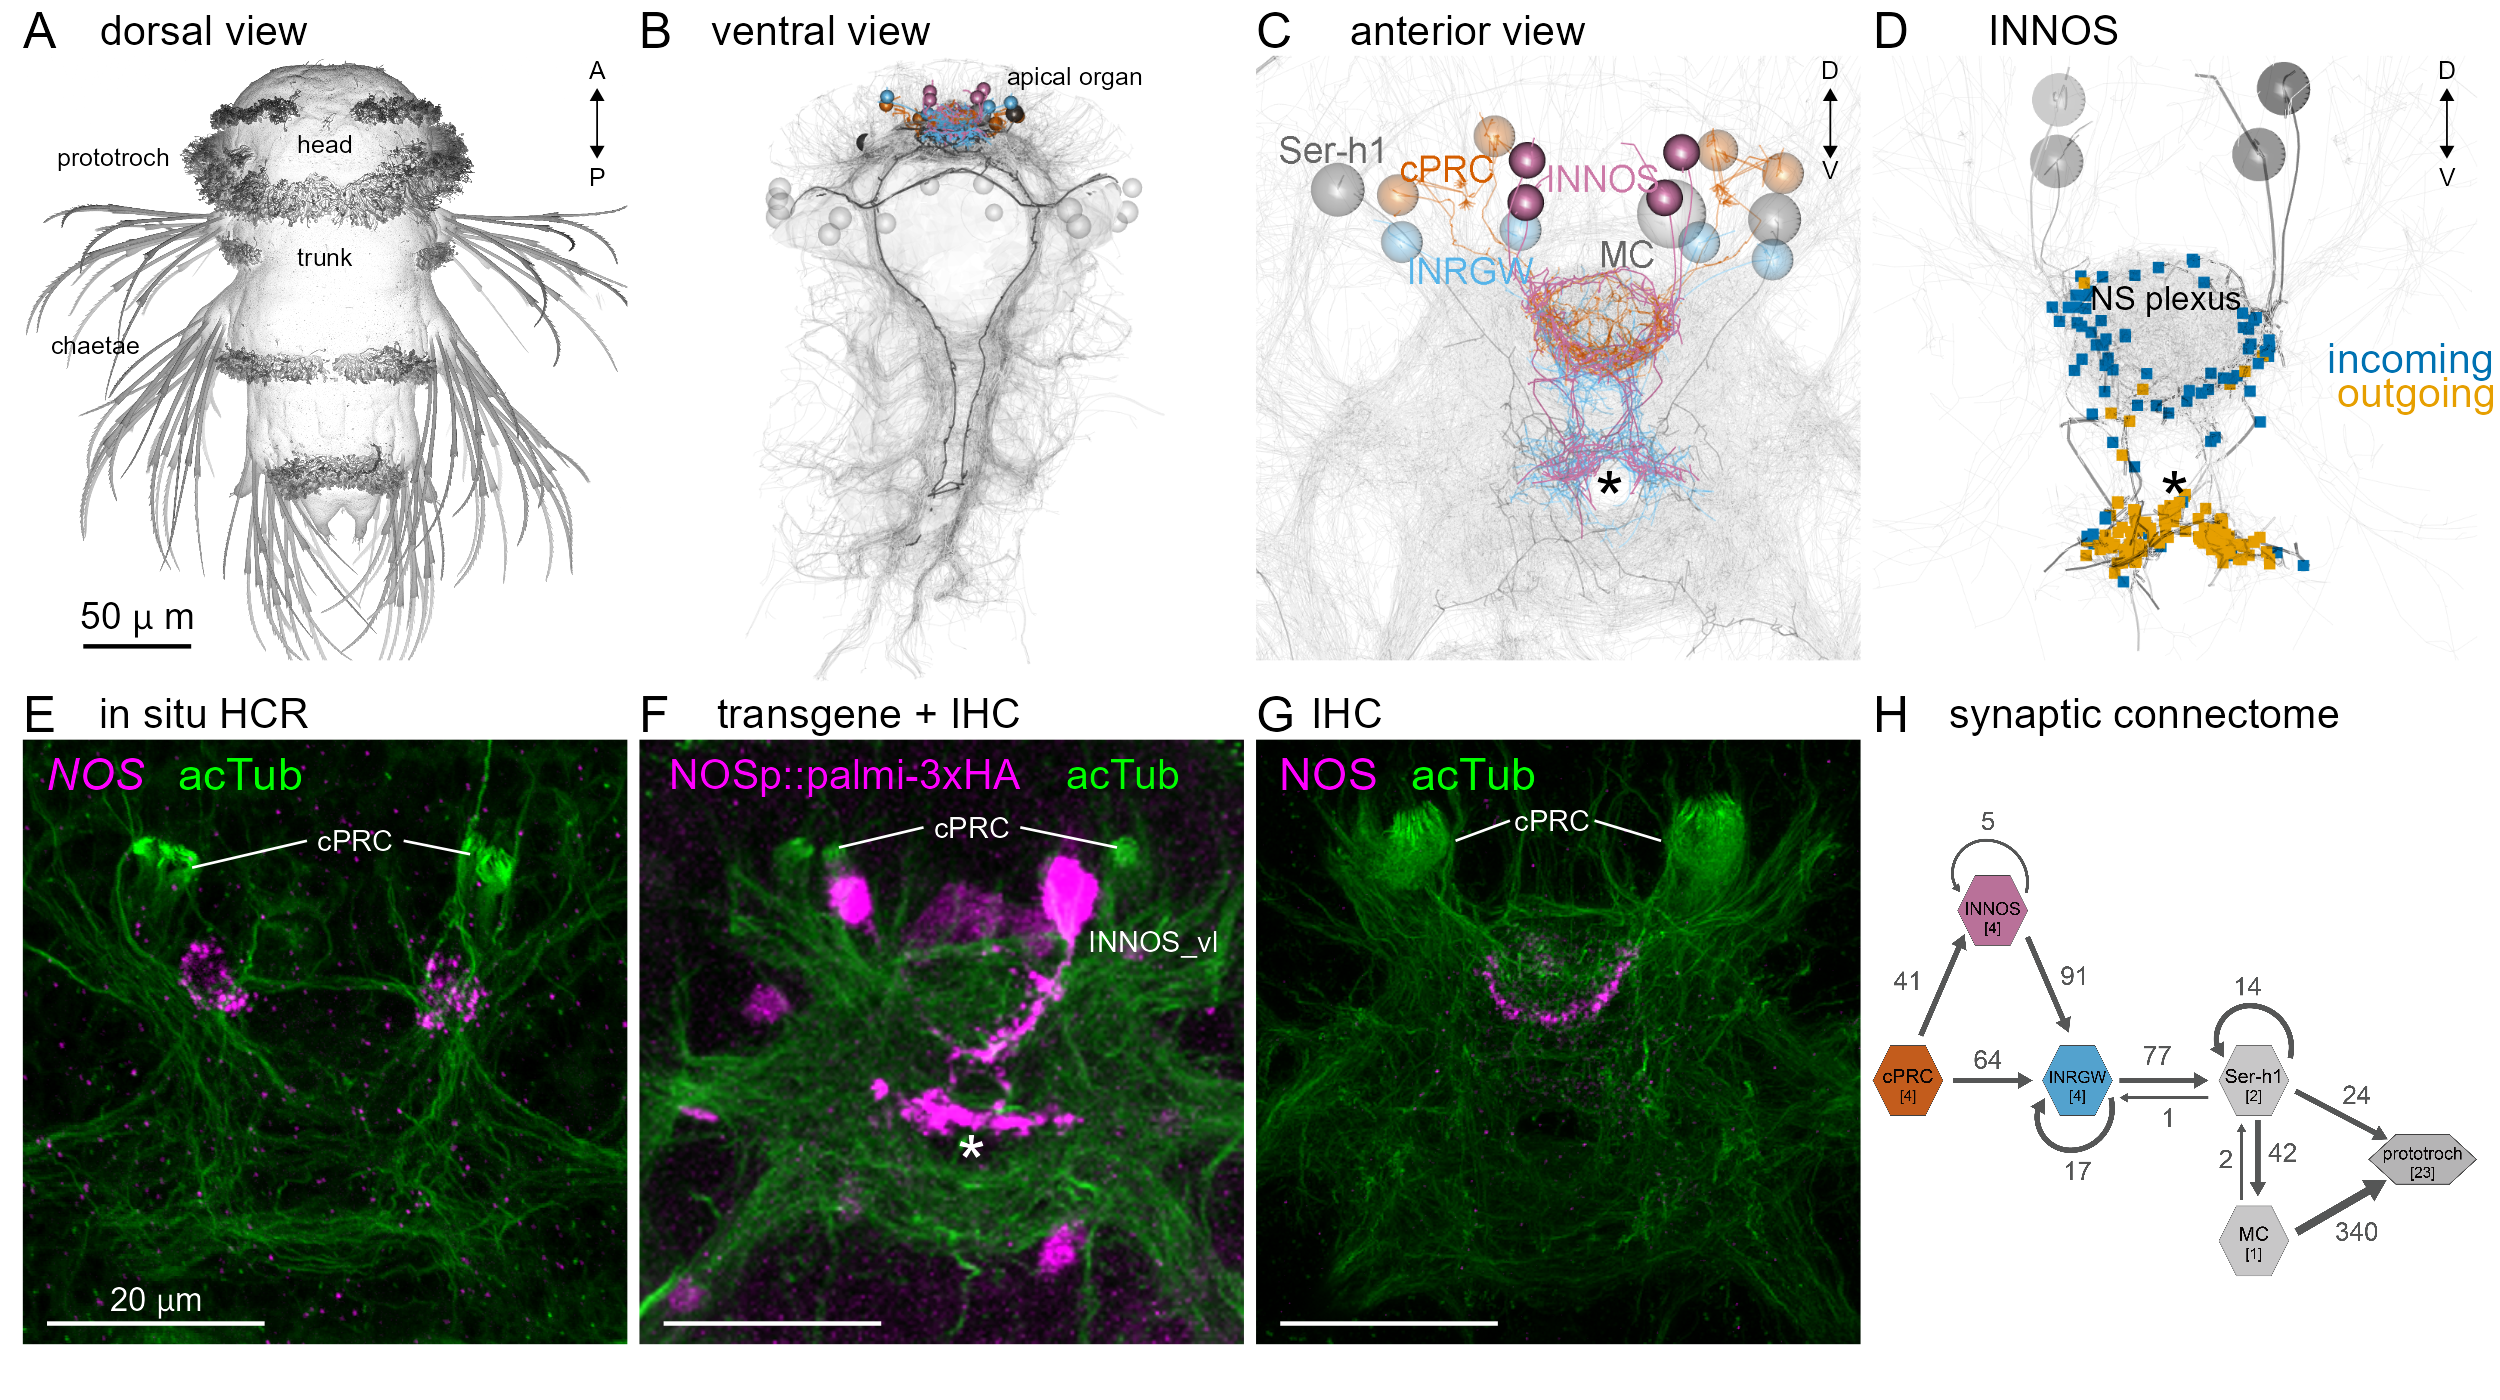
\includegraphics[width=25in]{figures/Fig1} \caption{**Figure 1. Identification of NOS-expressing interneurons (INNOS) within the cPRC circuit.** **(A)** Scanning electron microscopy image of a three-day-old *Platynereis* larva. **(B, C)** Volume rendering of the neuron types (cPRC, INNOS, INRGWa, Ser-h1 and MC) in the cPRC circuit reconstructed from a whole-body transmission electron microscopy volume of a three-day-old larva. Neurite skeletons are shown with cell-body positions represented by spheres. Projections of all neurons in the body are shown in grey to highlight the neuropils. The outline of the yolk is also indicated in grey. In B, nuclei positions of the prototroch head ciliary band are shown as grey spheres. **(D)** Expression of the *NOS* gene detected by in situ HCR (magenta) in a two-day-old larva (anterior view). Antibody staining for acetylated α-tubulin (acTub: green) highlights cPRC cilia and the neuropil. **(E)** Expression of a *NOS* reporter (NOSp::palmi-3xHA: magenta) labelled with an anti-HA antibody in a two-day-old larva (anterior view). Antibody staining for acetylated α-tubulin (acTub: green) highlights cPRC cilia and the neuropil. **(F)** Synaptic wiring diagram of the cPRC circuit. Hexagons represent cell groups, with the number of cells per group shown in square brackets. Arrows represent the summed number of synaptic contacts between cell groups. Arrow thickness is proportional to the number of synapses.}\label{fig:unnamed-chunk-1}
\end{figure}

\textbf{Nitric oxide is produced during UV/violet stimulation of the
cPRCs}

The expression of \emph{NOS} in the INNOS interneurons in the cPRC
circuit suggests that NO signalling may be involved in
UV/violet-avoidance. To test this, first we asked whether NO is produced
during UV/violet stimulation of the larvae. We injected the fluorescent
NO-reporter DAF-FM into zygotes and imaged two-day-old larvae while
exposing the region of cPRC cilia to 405 nm violet light. To mark cell
outlines, we coinjected mRNA encoding a red-fluorescent reporter
(RGECO), allowing the identification of the cPRCs. Following light
stimulation in the region of the ramified cilia of the cPRCs, we
detected an increase in DAF-FM fluorescence in the anterior
neurosecretory neuropil, the region of INNOS projections. This increase
did not occur in larvae where we illuminated a control area (Figure 2).

\begin{figure}
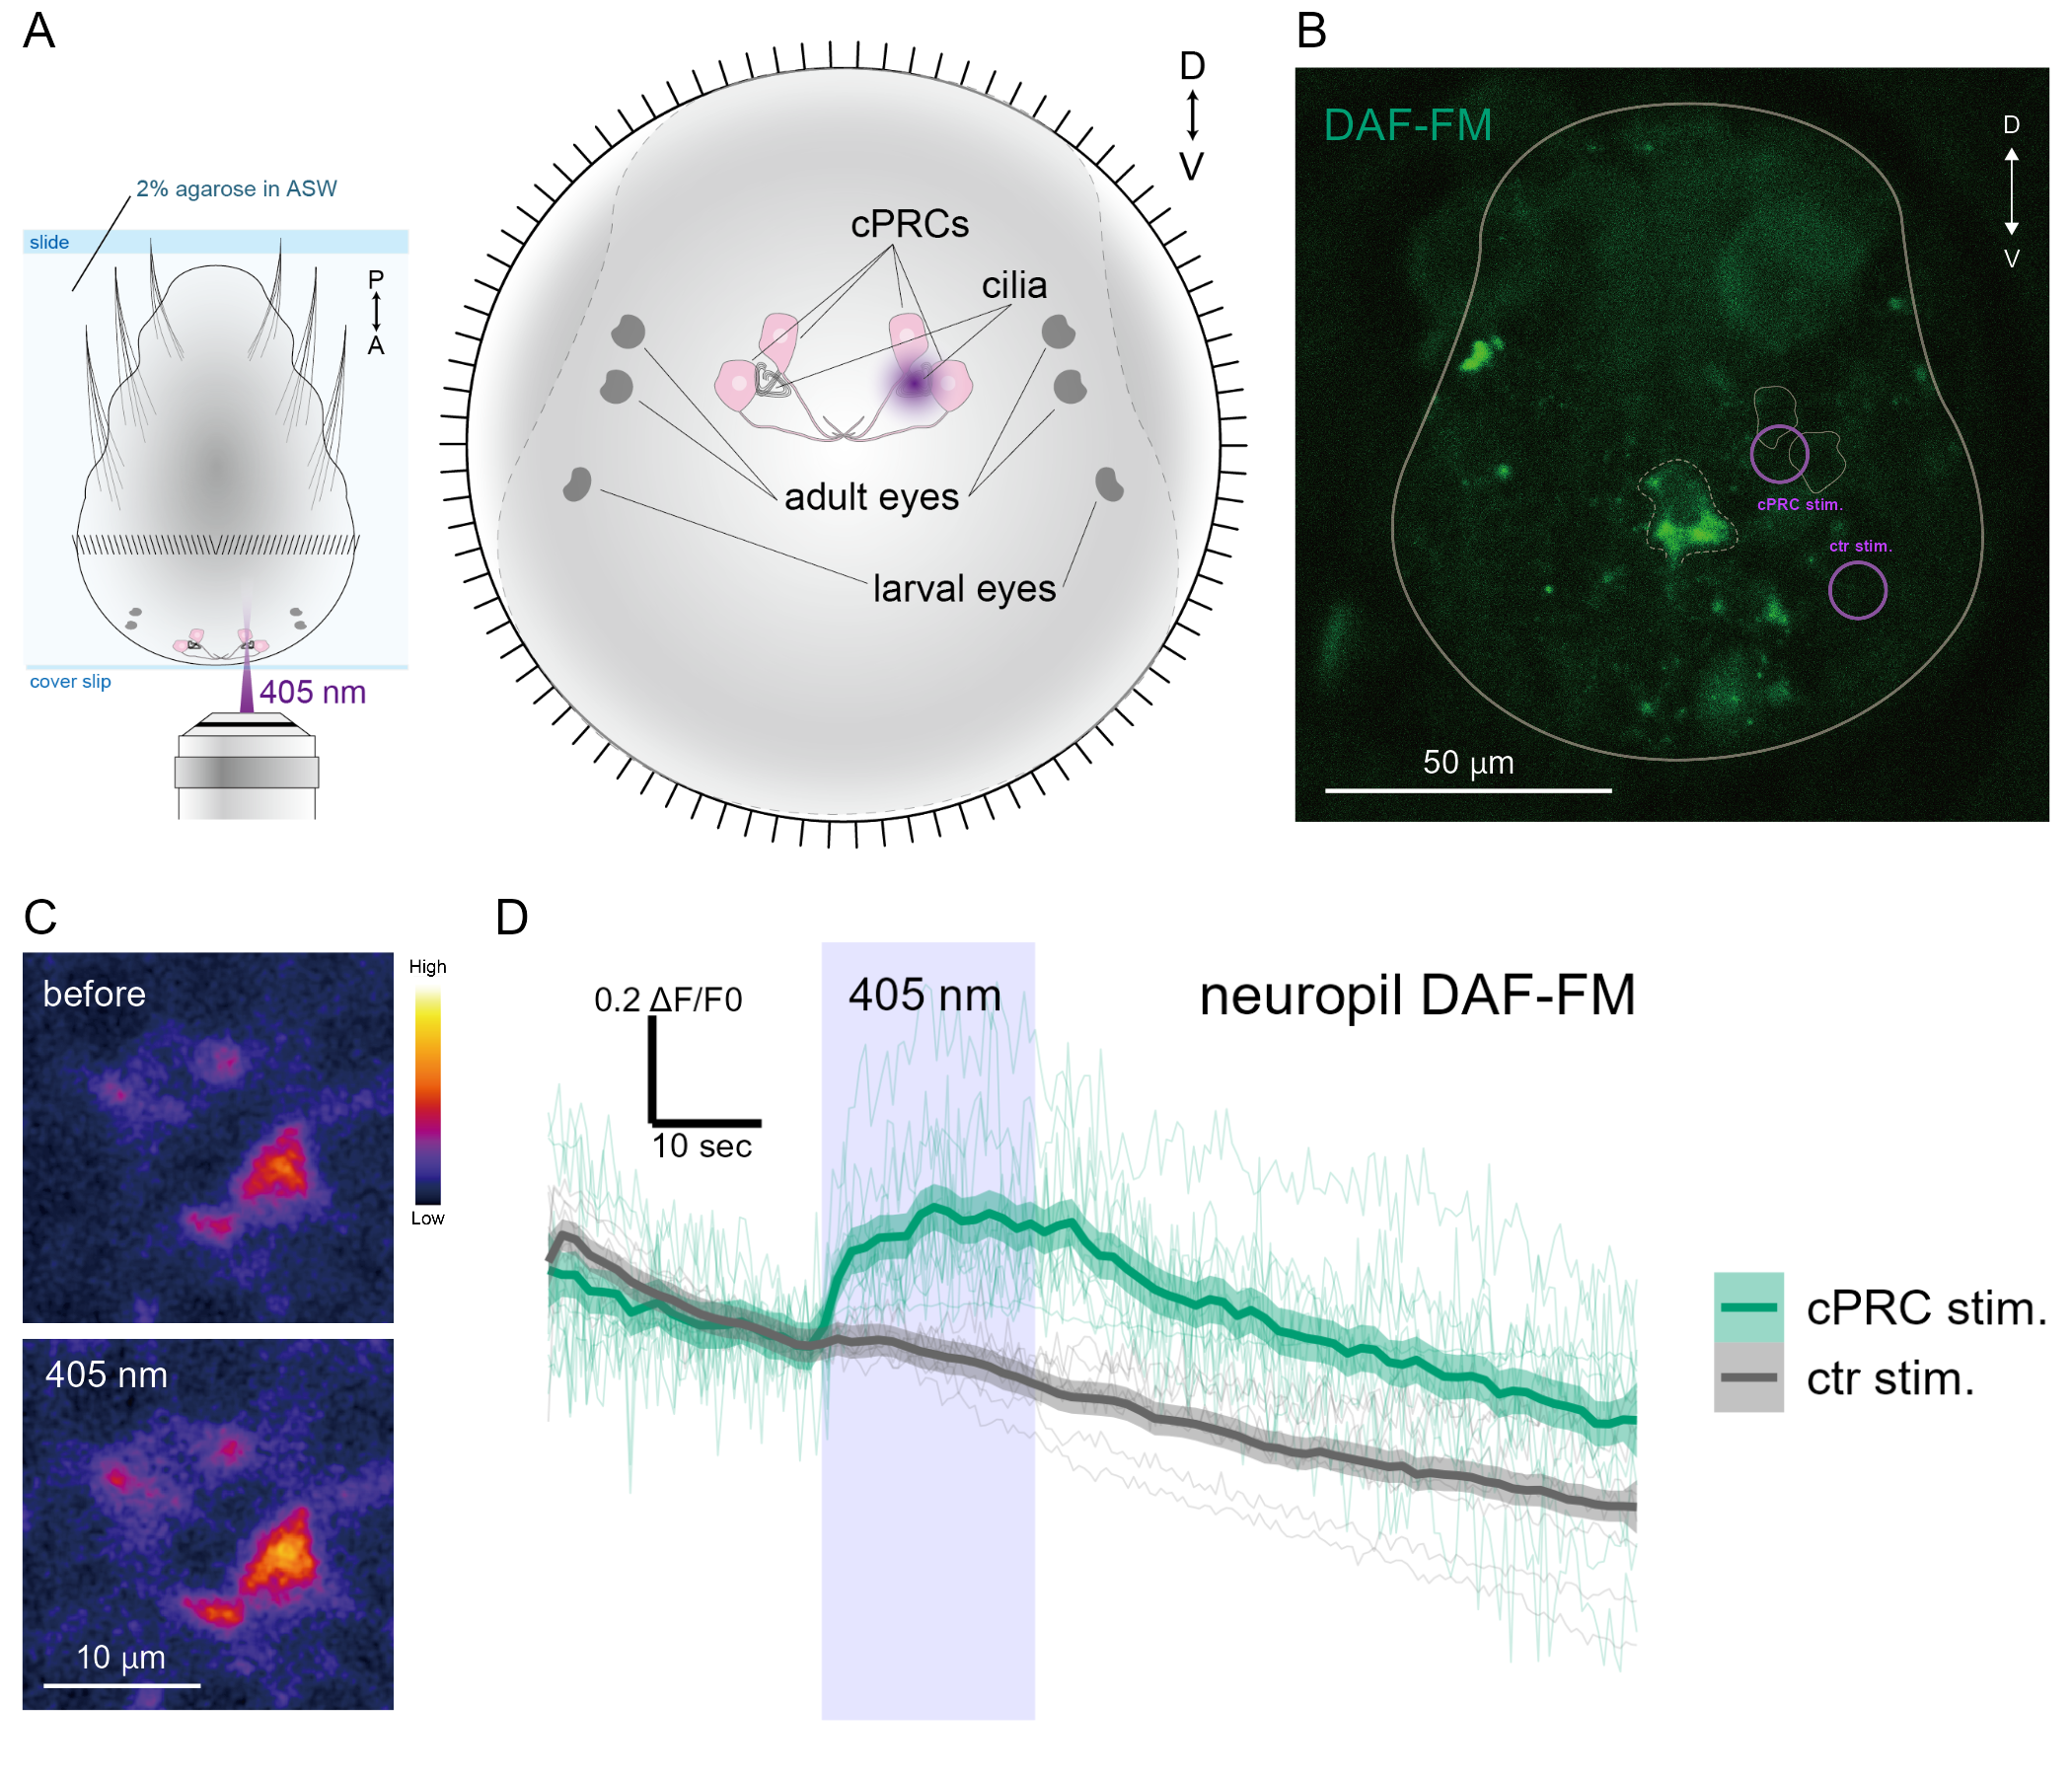
\includegraphics[width=29.17in]{figures/Fig2} \caption{**Figure 2. NO produced by UV/violet stimulation to cPRCs.** **(A)** DAF-FM fluorescence in the region of the neurosecretory neuropil. The white line indicates the outline of the larva. The dashed line corresponds to the area where fluorescence was quantified. Circles indicate the location of cPRC and control stimulation. cPRCs are marked by thin lines. **(B)** Changes in DAF-FM fluorescence before and during 405 nm light stimulation. **(C)** Changes in DAF-FM fluorescence over time during 405 nm stimulation of the cPRCs (green) or a control area (ctr: gray). The purple box indicates the duration of 405 nm stimulation. Individual traces normalized (ΔF/F0) are shown as thin lines. Thick lines show the mean value with 0.95 confidence intervals. N = 9 larvae for control and 11 for cPRC stimulation.}\label{fig:unnamed-chunk-2}
\end{figure}

\textbf{Nitric oxide signalling mediates UV-avoidance behaviour}

We next tested whether NO signalling regulates UV/violet avoidance. To
achieve this, we generated two \emph{Platynereis} \emph{NOS} knockout
lines with the CRISPR/Cas9 method. We recovered two deletions
(NOSΔ11/Δ11 and Δ23/Δ23), both frame-shift mutations leading to an early
stop codon and thus likely representing null alleles (Figure 3---figure
supplement 1A). We could establish a homozygous line for both mutations
indicating that NOS is not an essential gene in \emph{Platynereis}. To
quantify UV avoidance, we recorded the trajectories of freely swimming
wild type and mutant larvae in vertical columns, illuminated laterally
from two opposite sides with 395 nm UV light (Figure 3A and Figure
3---figure supplement 1B). As previously shown, wild-type larvae swim
downward following non-directional UV/violet light stimulation (Verasztó
et al., 2018). In contrast, both two- and three-day-old homozygous
\emph{NOS}-mutant larvae showed a strongly diminished UV-avoidance
response (Figure 3A, B and Figure 3---figure supplement 1B,C). This
phenotype is similar to the defective UV-avoidance of \emph{c-opsin1}
mutant larvae (Verasztó et al., 2018) and reveals a requirement for NOS
in UV-avoidance behaviour. Wild type but not mutant larvae also showed
an increase in swimming speed under UV light that may be due to downward
swimming trajectories (swimming in the direction of gravity) (Figure 3B
and Figure 3---figure supplement 1C). We also tested directional
phototaxis, by exposing larvae to 480 nm directional collimated light
from the top of the column. Three-day-old but not two-day-old
\emph{NOS}-mutant larvae also showed reduced phototactic behaviour,
suggesting a function for \emph{NOS} in the visual eyes that mediate
three-day-old phototaxis (Randel et al., 2014) (Figure 3D and Figure
3---figure supplement 1G).

To distinguish between an acute and developmental function of NOS in
light responses, we next tested larvae exposed to the NOS inhibitor
L-NAME. Larvae incubated for 5 min in 0.1 mM or 1 mM L-NAME showed a
dose-dependent inhibition of UV avoidance. In contrast, phototaxis was
not affected (Figure 3C, E). Overall, our results indicate an acute
requirement for NOS signalling in UV-avoidance and a possible indirect,
developmental role in the visual system, reminiscent of the function of
NO signalling in \emph{Drosophila} eye development (Gibbs and Truman,
1998).

\begin{figure}
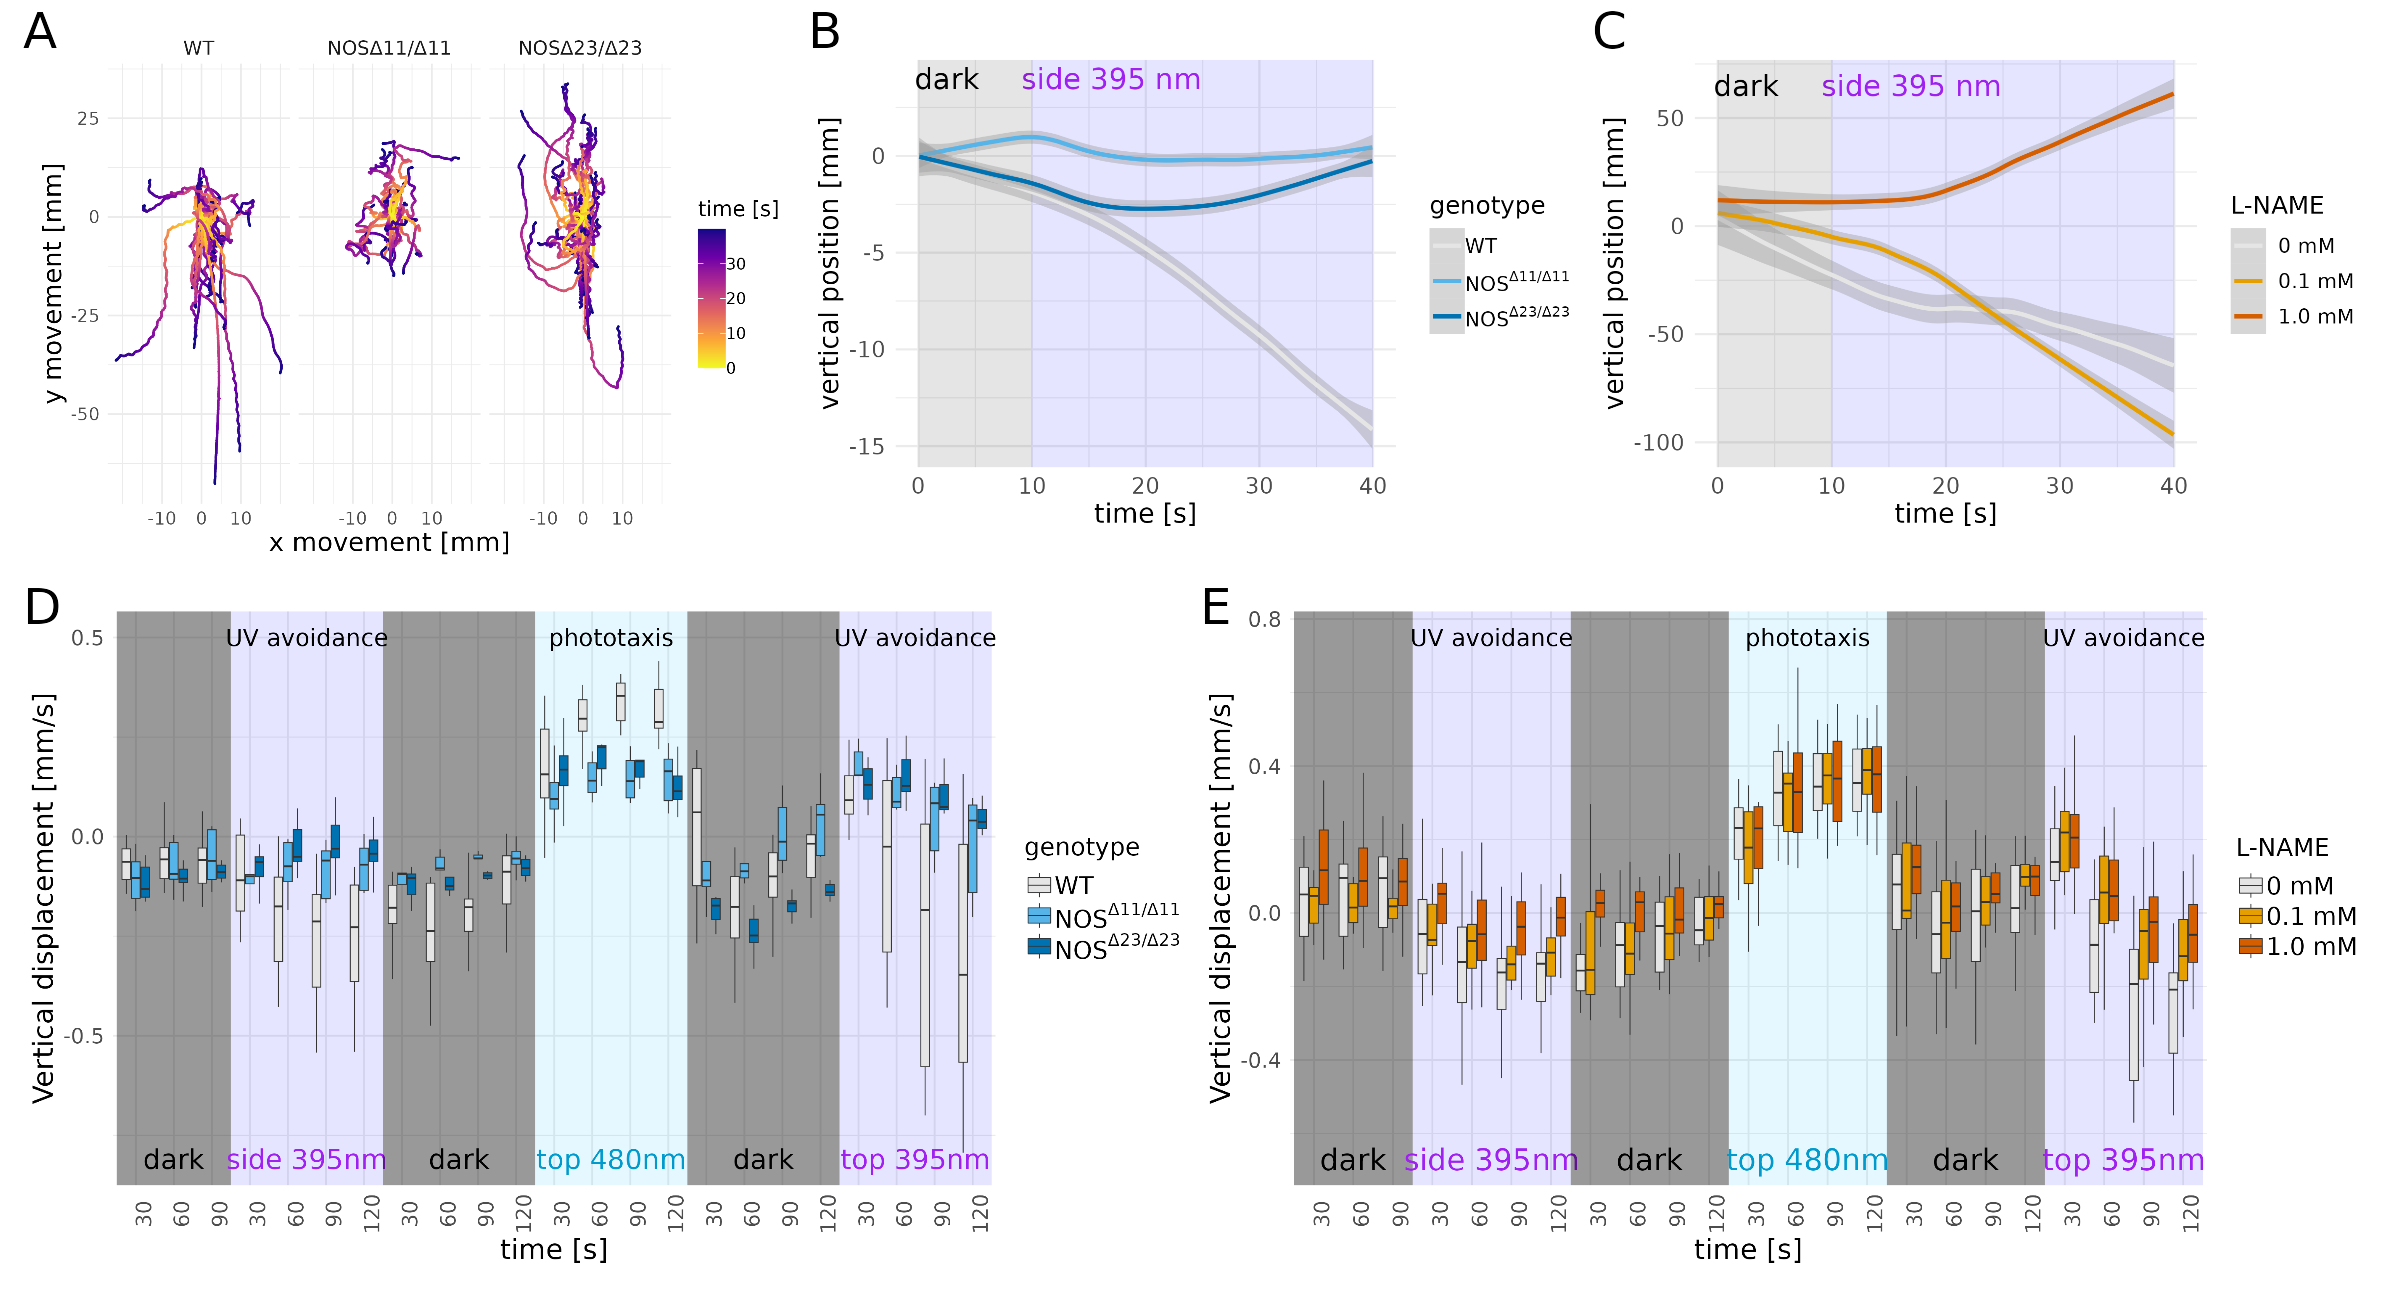
\includegraphics[width=33.33in]{figures/Fig3} \caption{**Figure 3. NOS is required for UV avoidance in *Platynereis* larvae.**  **(B)** Swimming trajectories of wild type (WT, n=32) and NOS mutant (NOSΔ11/Δ11, n=26 and NOSΔ23/Δ23, n=47) three-day-old larvae. All trajectories start at 0 x and y position and time 0 corresponding to 10 sec after the onset of 395 nm stimulation from the side. **(B)** Vertical position of batches of wild type and mutant three-day-old larvae over time under 395 nm UV stimulation. The starting position of each larval trajectory was set to 0. **(C)** Vertical position of batches of control and L-NAME-treated (0.1 and 1 mM) three-day-old larvae over time under 395 nm UV stimulation. The starting position of each larval trajectory was set to 0. **(D)** Vertical displacement in 30 sec bins of wild type and mutant (NOSΔ11 and NOSΔ23) three-day-old larvae stimulated with 395 nm light from the side, 488 nm light from the top and 395 nm light from the top. **(E)** Vertical displacement in 30 sec bins of control and L-NAME-treated (0.1 and 1 mM) three-day-old larvae stimulated with 395 nm light from the side, 488 nm light from the top and 395 nm light from the top.}\label{fig:unnamed-chunk-3}
\end{figure}

\textbf{NO retrograde signalling tunes cPRC responses to UV/violet
stimulation}

To investigate how NO signalling alters the dynamics of the cPRC
circuit, we carried out calcium imaging experiments. We ubiquitously
expressed the calcium sensor GCaMP6s in larvae and imaged calcium
signals during 405 nm stimulation of the cPRCs. As we have shown
previously, a 20-sec local stimulation of cPRC cilia led to a transient
increase in cPRC calcium levels, followed by a transient decrease
(Verasztó et al., 2018). After \textasciitilde20-sec, calcium levels in
cPRCs were raising again, reaching higher levels than at the start of
the stimulus -- a response that may involve depolarisation (Figure 4A,
B). This activation phase occurs after the 20 sec stimulation period and
is likely due to a delayed neuroendocrine feedback (Verasztó et al.,
2018). To determine whether NO mediates such a feedback, we repeated the
experiment in \emph{NOS}-mutant larvae. While we detected the initial
activation phase followed by inhibition, in homozygous
\emph{NOS}-mutants for both CRISPR alleles this was not followed by
delayed activation. Instead, calcium levels dropped to a low
steady-state level (Figure 4A, B). We thus identified a requirement for
NO signalling in the late-phase activation of cPRCs.

\textbf{Two unconventional guanylyl cyclases are expressed in the cPRCs}

We aimed next to identify the NO receptor in the cPRCs. NO generally
acts via soluble guanylate cyclases (sGC), belonging to the guanylate
cyclase family with a CYC domain (PFAM domain: PF00211). NO binding to
the heme group of sGC leads to increased cyclic guanosine monophosphate
(cGMP) production. Analysis of sGCs in \emph{Platynereis} indicated that
these genes are not expressed in any of the cells of the cPRC circuit
(Verasztó et al., 2017). Recently, Moroz and coworkers reported an
atypical but widely conserved family of guanylyl cyclases with a NIT
(nitrite/nitrate sensing) domain (PF08376) (NIT-GC) as potential
mediators of NO signalling (Moroz et al., 2020). To identify NIT-GCs in
\emph{Platynereis}, we searched transcriptome resources and retrieved 15
potential NIT-GC homologs (Figure 4---figure supplement 1 and 2). To
analyse the relationship of these sequences to metazoan NIT-GCs, we
retrieved protein sequences with a CYC domain from the transcriptome and
genome databases of 45 metazoan and 2 choanoflagellate species. We
carried out cluster analysis and did phylogenetic reconstruction on a
group of membrane-bound guanylyl cyclases with sGCs as an outgroup. In
agreement with Moroz et al. (Moroz et al., 2020), we found a group of
GCs with NIT domains with representatives in placozoans, cnidarians,
some ecdysozoans, echinoderms, and lophotrochozoans. The 15
\emph{Platynereis} sequences belonged to several deeply diverged clades
in the phylogenetic tree (Figure 4---figure supplement 1 and 2).

To characterise the expression of NIT-GCs, we used previously published
spatially mapped single-cell transcriptome data (Achim et al., 2015;
Williams et al., 2017). Among the 15 NIT-GCs, two showed high and
specific expression in the cPRCs and one was expressed in the INNOS
cells (Figure 4---figure supplement 2). In the single-cell data, we
could identify the cPRCs by the specific expression of \emph{c-opsin1}
and the \emph{pedal-peptide2 neuropeptide precursor} (\emph{MLD
proneuropeptide}), previously described cPRC markers (Arendt et al.,
2004; Williams et al., 2017) (Figure 4---figure supplement 3A). The
INNOS cells were identified by NOS expression and spatial mapping in the
brain (Achim et al., 2015). We decided to focus on two NIT-GCs expressed
in the cPRCs and with a full-length sequence, \emph{NIT-GC1} and
\emph{NIT-GC2}. To confirm the single-cell data, we first carried out in
situ hybridisation chain reaction (HCR) with probes for \emph{NIT-GC1}
and \emph{NIT-GC2} mRNA. Both genes were specifically expression in the
four cPRCs, as confirmed by co-labeling with an acetylated α-tubulin
antibody and with an HCR probe against \emph{pedal peptide 2/MLD
proneuropeptide} (Figure 4C, D and Figure 4---figure supplement 3A-C).
To analyse the subcellular localisation of NIT-GC1 and NIT-GC2 at the
protein level, we raised and affinity-purified polyclonal antibodies
against a specific peptide sequence from both proteins. In
immunostainings, we found that NIT-GC1 was localise to the region
corresponding to the axonal projections of the cPRCs in the anterior
neurosecretory plexus (Figure 4E). Co-immunostaining with the rabbit
NIT-GC1 antibody and a custom rat antibody raised against
\emph{Platynereis} NOS revealed the localisation of both proteins in
dots in the neurosecretory neuropil (Figure 4---figure supplement 3D).
In contrast, NIT-GC2 specifically labelled the ramified sensory cilia of
the cPRCs (Figure 4F). These different subcellular localisations suggest
that the two NIT-GCs are involved in different intracellular signalling
processes in the ciliary and axonal regions of the cPRCs.

\textbf{NIT-GC1 produces cGMP in an NO-dependent manner}

To further characterise these atypical guanylyl cyclases, we focused on
NIT-GC1 and carried out in vitro experiments. In bacteria, NIT domains
are thought to regulate cellular functions in response to intra- or
extracellular nitrate and nitrite. NIT-GC1 has a NIT domain and a highly
conserved cyclase domain that is expected to catalyse cGMP synthesis
(Figure 4G). The NIT domain may render NIT-GC1 dependent on NO signals.
To test this, we co-expressed the cGMP indicator Green cGull (Matsuda et
al., 2016) and NIT-GC1 in cultured COS-7 (monkey kidney) cells, a cell
line with minimal endogenous sGC activity (Matsuda et al., 2016). For
balanced expression, we used a single plasmid with the two open-reading
frames separated by the 2A self-cleaving peptide (Figure 4H).
Application of the NO donor SNAP lead to increased Green cGull
fluorescence, an effect we did not observe when cells were exposed to
DMSO or when Green cGull was expressed alone (Figure 4I-K). To test
whether this effect is dependent on the NIT domain, we also tested a
deletion construct of NIT-GC1 lacking the NIT domain (Figure 4G). Cells
expressing this construct and Green cGull did not show an increased
fluorescence of the cGMP reporter when exposed to SNAP (Figure 4L).
These results indicate that NIT-GC1 is able to catalyse cGMP production
in an NO-dependent manner and this function requires the NIT domain.
These results establish NIT-GC1 as a biochemical sensor of NO or its
derivatives.

\textbf{NIT-GC1 is required for NO-mediated retrograde signalling to
cPRCs during the UV response}

To test the in vivo function of NIT-GC1 and NIT-GC2 in cPRC responses,
we combined calcium imaging with morpholino-mediated knockdowns. We used
two translation-blocking morpholinos for each \emph{NIT-GC} gene and
tested knockdown efficiency by immunostaining injected animals with the
NIT-GC1 and NIT-GC2 antibodies (Figure 4---figure supplement 3E,F). For
both genes, the morpholinos led to a strong reduction in the respective
antibody signal, confirming efficient knockdown and antibody
specificity.

In NIT-GC1 morphant larvae, the delayed activation of cPRCs following
405 nm stimulation did not occur (Figure 4M). This phenotype is similar
to the phenotype of \emph{NOS} mutants suggesting that NIT-GC1 acts as
the NO sensor in cPRCs to drive their delayed activation. This could
occur via increased cGMP production and the opening of a
cyclic-nucleotide-gated ion channel (CNG) specific to cPRCs (Tosches et
al., 2014). NIT-GC2 morphant larvae, in contrast, showed a step-up
increase in calcium following light stimulation (Figure 4N). The calcium
signal decayed during stimulation and was off after light off. These
data support an essential role for ciliary-localised NIT-GC2 in
suppressing cPRC calcium following its transient rise at stimulus onset.
Overall, these knockdown experiments revealed different signalling
mechanisms for the two NIT-GCs that may be due to their different
subcellular localisations.

\begin{figure}

\includegraphics[width=38.89in]{figures/Fig4} \caption{**Figure 4. NOS and two NIT-GCs shape calcium signals during cPRC UV/violet response.** **(A, B)** GCaMP6s signals in cPRCs in wild type and *NOS* mutant (A, NOSΔ11/Δ11, B, NOSΔ23/Δ23) larvae during 405 nm light stimulation. **(C, D)** In situ HCR for (C) *NIT-GC1* and (D) *NIT-GC2* (magenta) in three-day-old *Platynereis* larvae. Larvae were co-stained with an antibody against acetylated α-tubulin to label cPRC cilia and the neuropil (green). **(E, F)** Immunostaining for (E) NIT-GC1 and (F) NIT-GC2 (magenta), co-stained for acetylated α-tubulin (green). **(G)** The domain structure of *Platynereis* NIT-GC1 and the truncated NIT-GC1ΔNIT protein lacking the NIT domain. A predicted transmembrane region (TM) is shown in grey. **(H)** Schematic of the cell-based assay to detect cGMP production following the addition of an NO donor SNAP or DMSO as control. **(I-L)** Green cGull fluorescence over time for the four conditions tested. Individual responses and their mean with 0.95 confidence interval are shown (n > 6 cells). Intensities are normalized (ΔF/F0). The indicated chemicals were added at 2 min after the start of imaging (grey bars). **(M, N)** GCaMP6s signals in cPRCs in (M) NIT-GC1 and (N) NIT-GC2 morphant larvae during 405 nm light stimulation. Individual responses and their mean with 0.95 confidence interval are shown.}\label{fig:unnamed-chunk-4}
\end{figure}

\textbf{NO signalling shapes the dynamics of the cPRC circuit}

To investigate how NO and NIT-GC signalling influence the dynamics of
the cPRC circuit, we imaged calcium signals from postsynaptic neurons in
wild type, mutant and morphant larvae. We were able to image the
activity of all neurons in the cPRC circuit (INNOS, INRGWa, Ser-h1 and
MC). The MC cell was identified based on its position and intrinsic
activity (Verasztó et al., 2017). To unambiguously identify all other
cells from which we recorded calcium signals, we developed an on-slide
immunostaining method (Figure 5---figure supplement 1A). We used the
cell-specific antibody markers against RYamide (INNOS) (Figure
5---figure supplement 1B-D), RGWamide (INRGWa) and serotonin (Ser-h1)
(Conzelmann et al., 2011) to immunostain agar-embedded larvae following
calcium imaging. Based on the position of the nuclei, we could correlate
live and fixed samples at a single-cell precision (Figure 5A,B). Due to
the stereotypy of the larvae, we could also identify neurons based on
their position and calcium activity in activity-correlation maps (Figure
5C).

We first quantified the responses of the INNOS and INRGWa interneurons
during 405 nm stimulation of the cPRCs. In both wild type and
\emph{NOS}-mutant larvae, INNOS cells showed an increase in calcium
during stimulation (Figure 5D). In contrast, the INNOS response was flat
or slightly negative in NIT-GC2 morphant larvae (Figure 5E) revealing an
essential role for NIT-GC2-mediated cPRC suppression in INNOS
activation. INRGWa cells were initially inhibited during cPRC
stimulation, followed by a delayed activation paralleling the second
activation phase of cPRCs. This late INRGWa response was lacking in
\emph{NOS}-mutants (Figure 5F). In NIT-GC2 morphants, INRGWa cells
showed a transient increase in calcium that decayed after light off and
a delayed activation was not present (Figure 5G).

Next, we imaged calcium signals from Ser-h1 and MC neurons in wild type
and \emph{NOS} mutant larvae. Ser-h1 cells showed an activation profile
that correlated with cPRC activity, including a reduction in calcium
during stimulation followed by rebound, a response that was defective in
\emph{NOS} mutants (Figure 5I). MC cells showed sustained activation,
including a late-phase that was lacking in \emph{NOS} mutants (Figure
5I). These data suggest that during 405 nm stimulation the Ser-h1 cells
are inhibited and MC cells are activated, and this regulation is
NO-dependent. This pattern is expected to inhibit ciliary activity in
the prototroch but not in the other ciliary bands, triggering
NO-dependent downward swimming.

\begin{figure}
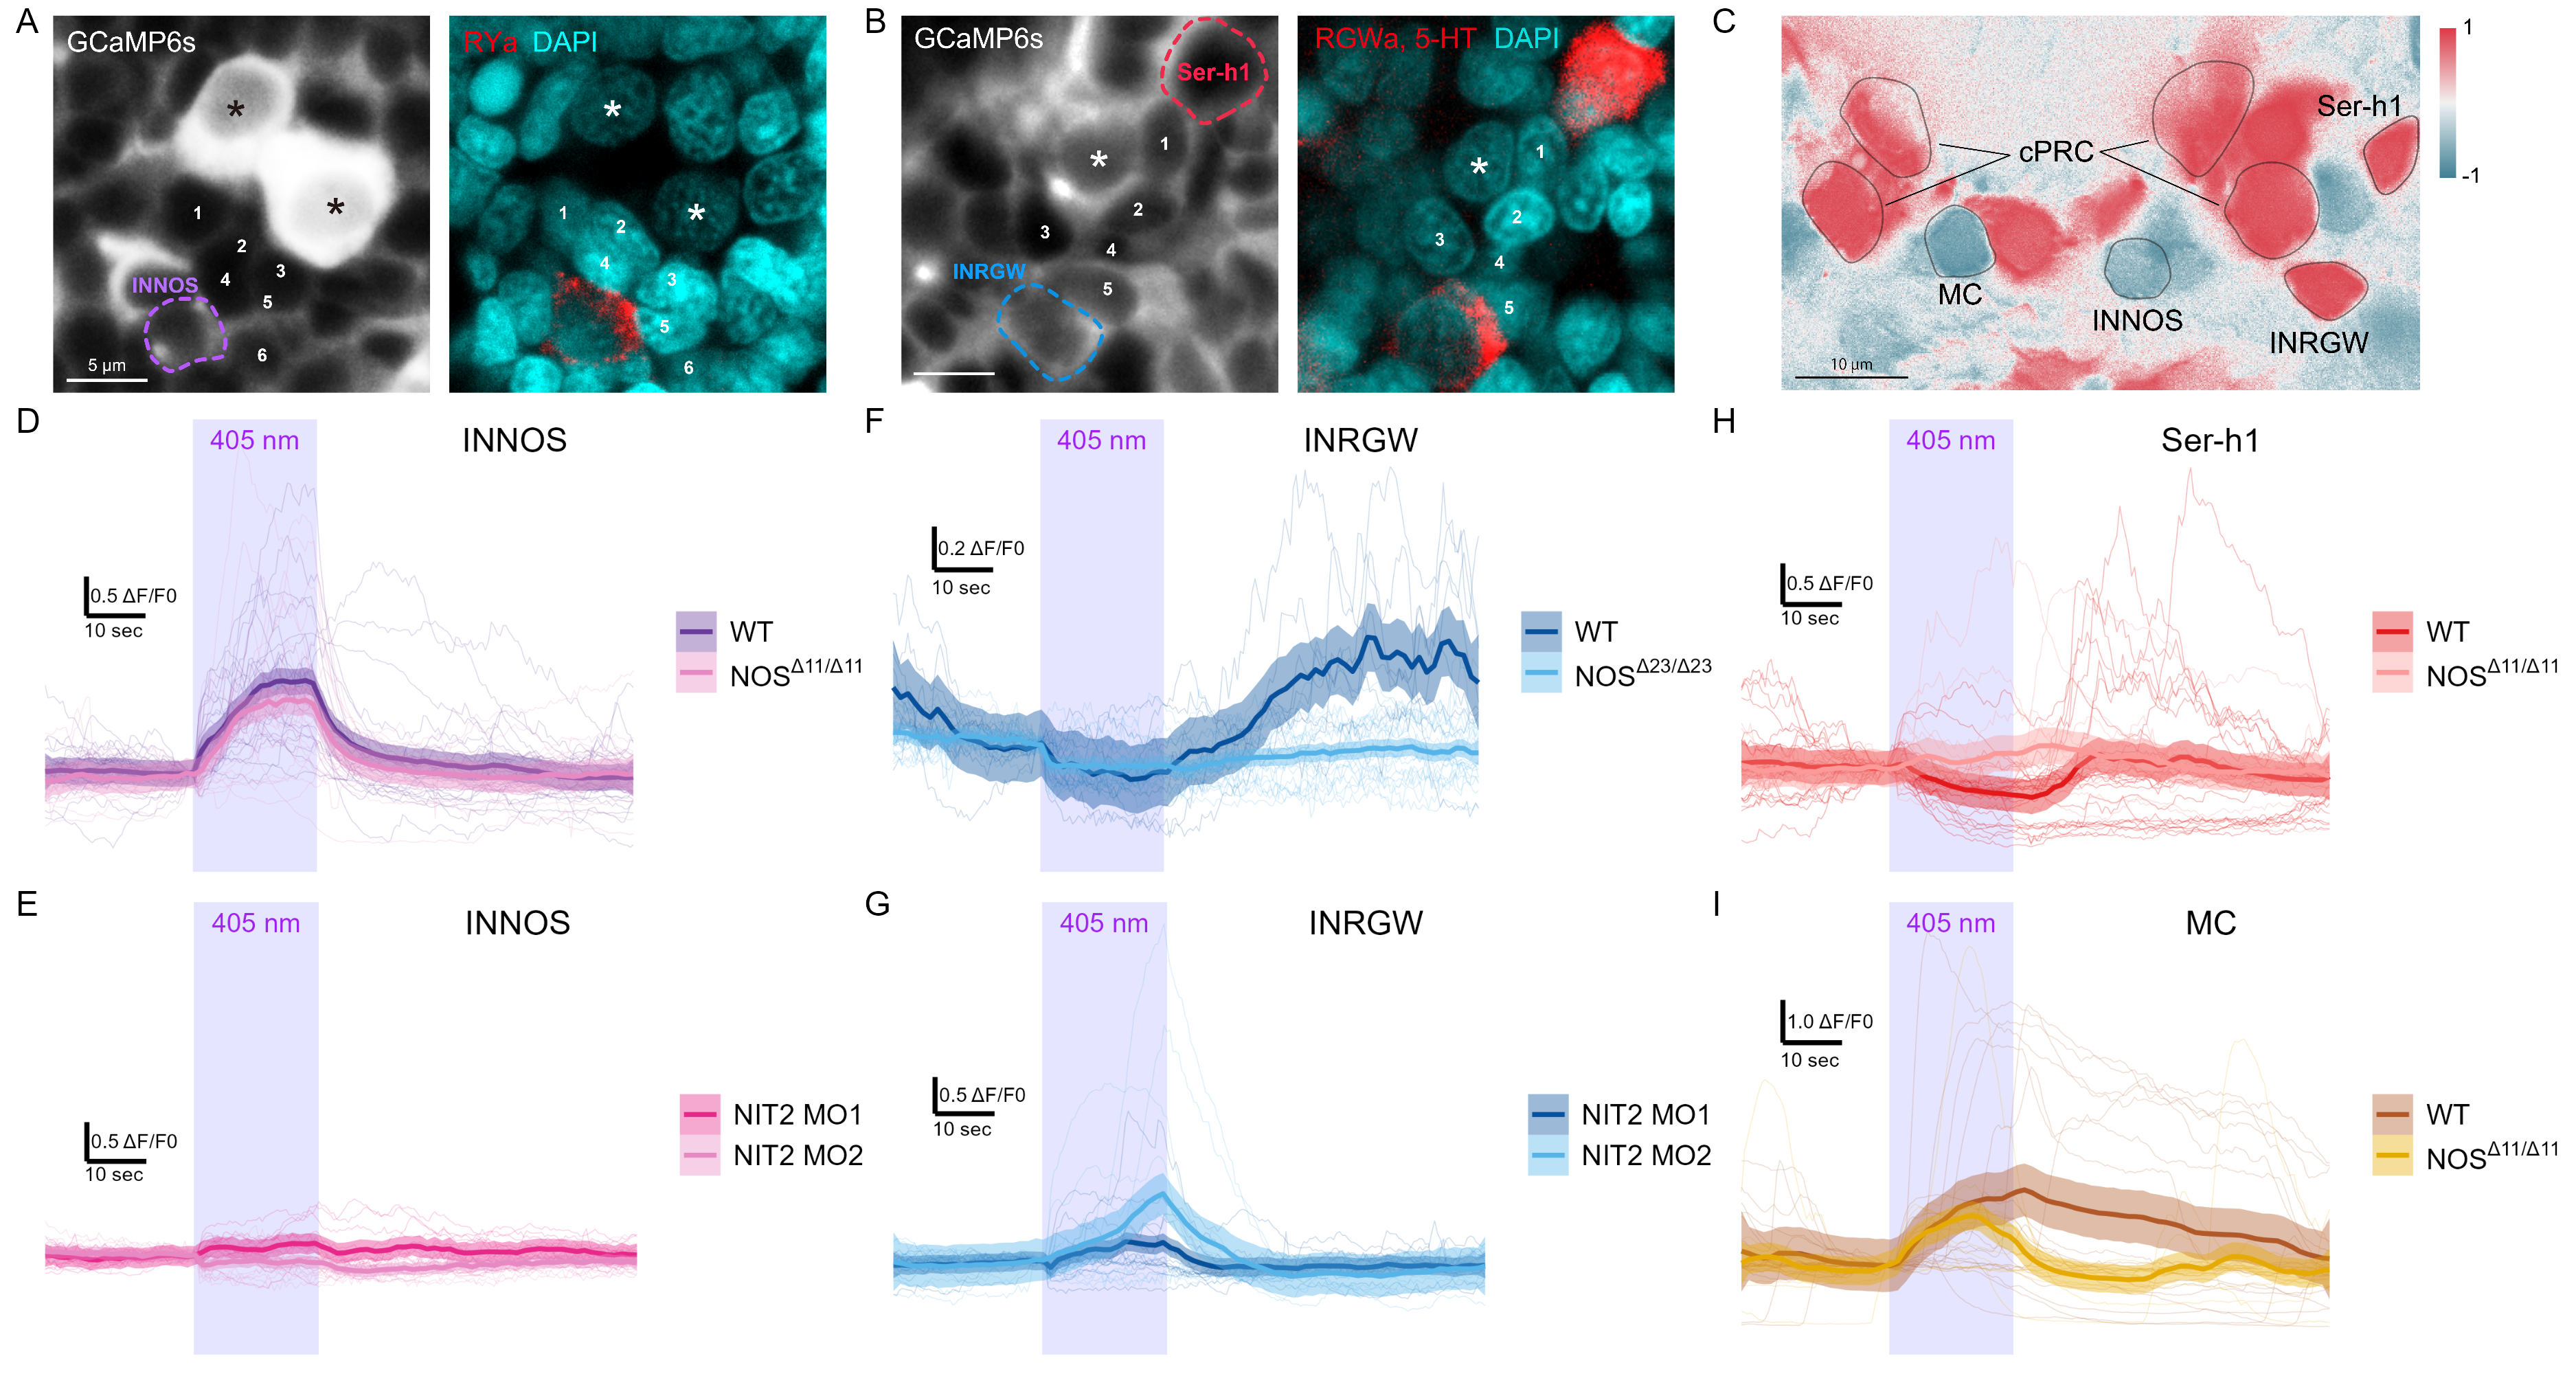
\includegraphics[width=52.08in]{figures/Fig5} \caption{**Figure 5. NOS- and NIT-GC2-dependent dynamics of the cPRC circuit.** **(A, B)** GCaMP6s imaging from cPRCs and INNOS cells (left panels) followed by on-slide immunostaining for (A) RYamide to label INNOS and (B) RGWamide+serotonin to label INRGWa and Ser-h1 (red). Nuclei are stained with DAPI (cyan). Asterisks indicate cPRC nuclei. Numbers mark the same cells in the GCaMP and immunostaining images matched by position. **(C)** Correlation map of neuronal activity of the cPRCs, INNOS, INRGWa, Ser-h1 and MC neurons. **(D)** GCaMP6s fluorescence in INNOS cells in wild type (WT) and NOSΔ11/Δ11 mutant larvae during 405 nm stimulation of the cPRC cilia. **(E)** GCaMP6s fluorescence in INNOS cells in NIT-GC2 morphant larvae during 405 nm stimulation. **(F)** GCaMP6s fluorescence in INRGWa cells in wild type and NOSΔ23/Δ23 mutant larvae during 405 nm stimulation. **(G)** GCaMP6s fluorescence in INRGWa cells in NIT-GC2 morphant larvae during 405 nm stimulation. **(H, I)** GCaMP6s fluorescence in (H) Ser-h1 cells and (I) the MC cell in wild type and NOSΔ11/Δ11 mutant larvae during 405 nm stimulation.}\label{fig:unnamed-chunk-5}
\end{figure}

\textbf{Mathematical modelling of cPRC-circuit dynamics}

To further analyse the dynamics of responses to UV light and formally
describe cPRC phototransduction, synaptic connections and NO retrograde
signalling, we developed a mixed cellular-circuit-level mathematical
model. We used our Ca2+ imagining data of cPRC, INNOS and INRGWa cells
collected in wild type, \emph{NOS} knockout, and \emph{NIT-GC2} morphant
larvae to formulate assumptions that are the basis of the proposed
model.

We model a direct c-opsin1-dependent response to UV leading to the
initial rise in Ca2+ levels. The mechanism of this signal is not known
but may include Gα and Gβ signalling, CNGAα channel activation or other
pathways. We further assume that in cPRC cells, Ca2+ levels increase
with cGMP. We model a decrease in cGMP and Ca2+ levels due to a
NIT-GC2-dependent pathway (Figre 6A). The effect of NO in cPRC cells is
captured by another term that describes a NIT-GC1 and NO-dependent
increase in cGMP. Based on the synaptic connectome, we infer a
feedforward coupling between cPRC cells and INNOS and INRGWa cells. The
proposed synaptic coupling is UV-dependent, decays linearly and is
suppressed in NIT-GC2 morphants (Figure 6A).

In the INNOS cells, we assume that excitatory synaptic input from cPRC
(or rebound from tonic inhibition) leads to a rise in Ca2+ leading to NO
production via NOS. This input is NIT-GC2-dependent. In the INRGWa
cells, we model a decrease in Ca2+ based on an inhibitory UV-dependent
synaptic signal from the cPRCs. We further assume the existence of
direct excitatory coupling between cPRC Ca2+ levels and INRGWa Ca2+ to
account for the late effects of cPRC on INRGWa (Figure 6A). The
UV-dependent and Ca2+-dependent signals may be mediated by different
transmitters released by cPRCs during distinct phases of their
activation cycle. In addition, we assume a direct inhibitory coupling
between INNOS Ca2+ and INRGWa Ca2+. Finally, in all variables, we
assumed a linear decay and constant production to set a steady state
(Figure 6A). Since the aim of the model is to capture the normalised
fluorescence data, the model is nondimensionalised. UV stimulation is
modelled as a square pulse. To find model parameters producing an output
fitting the experimental data we employed a global optimisation method
known as a genetic algorithm (GA).

Through this optimisation procedure, we found parameters that gave a
very good fit to our experimental data under all conditions. We could
fit to mean Ca2+ values but also individual calcium transients (Figure
6B, Figure 6--figure supplement 1). Our model only includes a minimal
set of parameters and assumptions of interactions that are required to
describe the dynamics of cPRC, INNOS and INRGWa in wild type and
loss-of-function conditions (Figure 6A, B). The model highlights that
cPRC phototransduction employs distinct pathways that operate on
different time scales and differentially influence cPRC Ca2+ levels. The
coupling between cPRCs and interneurons also requires different
signalling mechanisms, either through distinct neurotransmitters or
receptors expressed in the different cells.

To identify possible molecular pathways, we analysed single-cell
transcriptome data for cPRC, INNOS and INRGWa identified by spatial
mapping (Achim et al., 2015) and unique marker genes (Williams et al.,
2017). In cPRCs, we found transporters and synthetic enzymes indicating
cholinergic, glutaminergic, glycinergic, GABAergic and adrenergic
neurotransmission (Figure 6C). For each neurotransmitter, we also found
receptor-encoding genes expressed in INNOS and INRGWa (Figure 6C). The
two types of interneurons often expressed different subunits or types of
these receptors, indicating differential signalling (Figure 6C).

Based on these data, our experimental results and the mathematical
model, we assembled a minimal phototransduction and circuit diagram. The
components for which experimental data are available are shown in bold.
Other potential molecular players are also indicated (Figure 6D).

To generate new insights from the model, we asked how the duration and
intensity of UV stimulation influences signalling output, measured as
the magnitude, duration and time to maximum of the NO-dependent Ca2+
signal in the cPRCs. The model allowed us to test a large number of
conditions that would not have been feasible in single-larva
experiments. We found that the onset, magnitude and duration of the
NO-dependent signal scales with stimulus intensity and duration (Figure
6--figure supplement 2). This suggests an integratory function of NO
signalling that tunes circuit output to the strength of UV exposure.

\begin{figure}
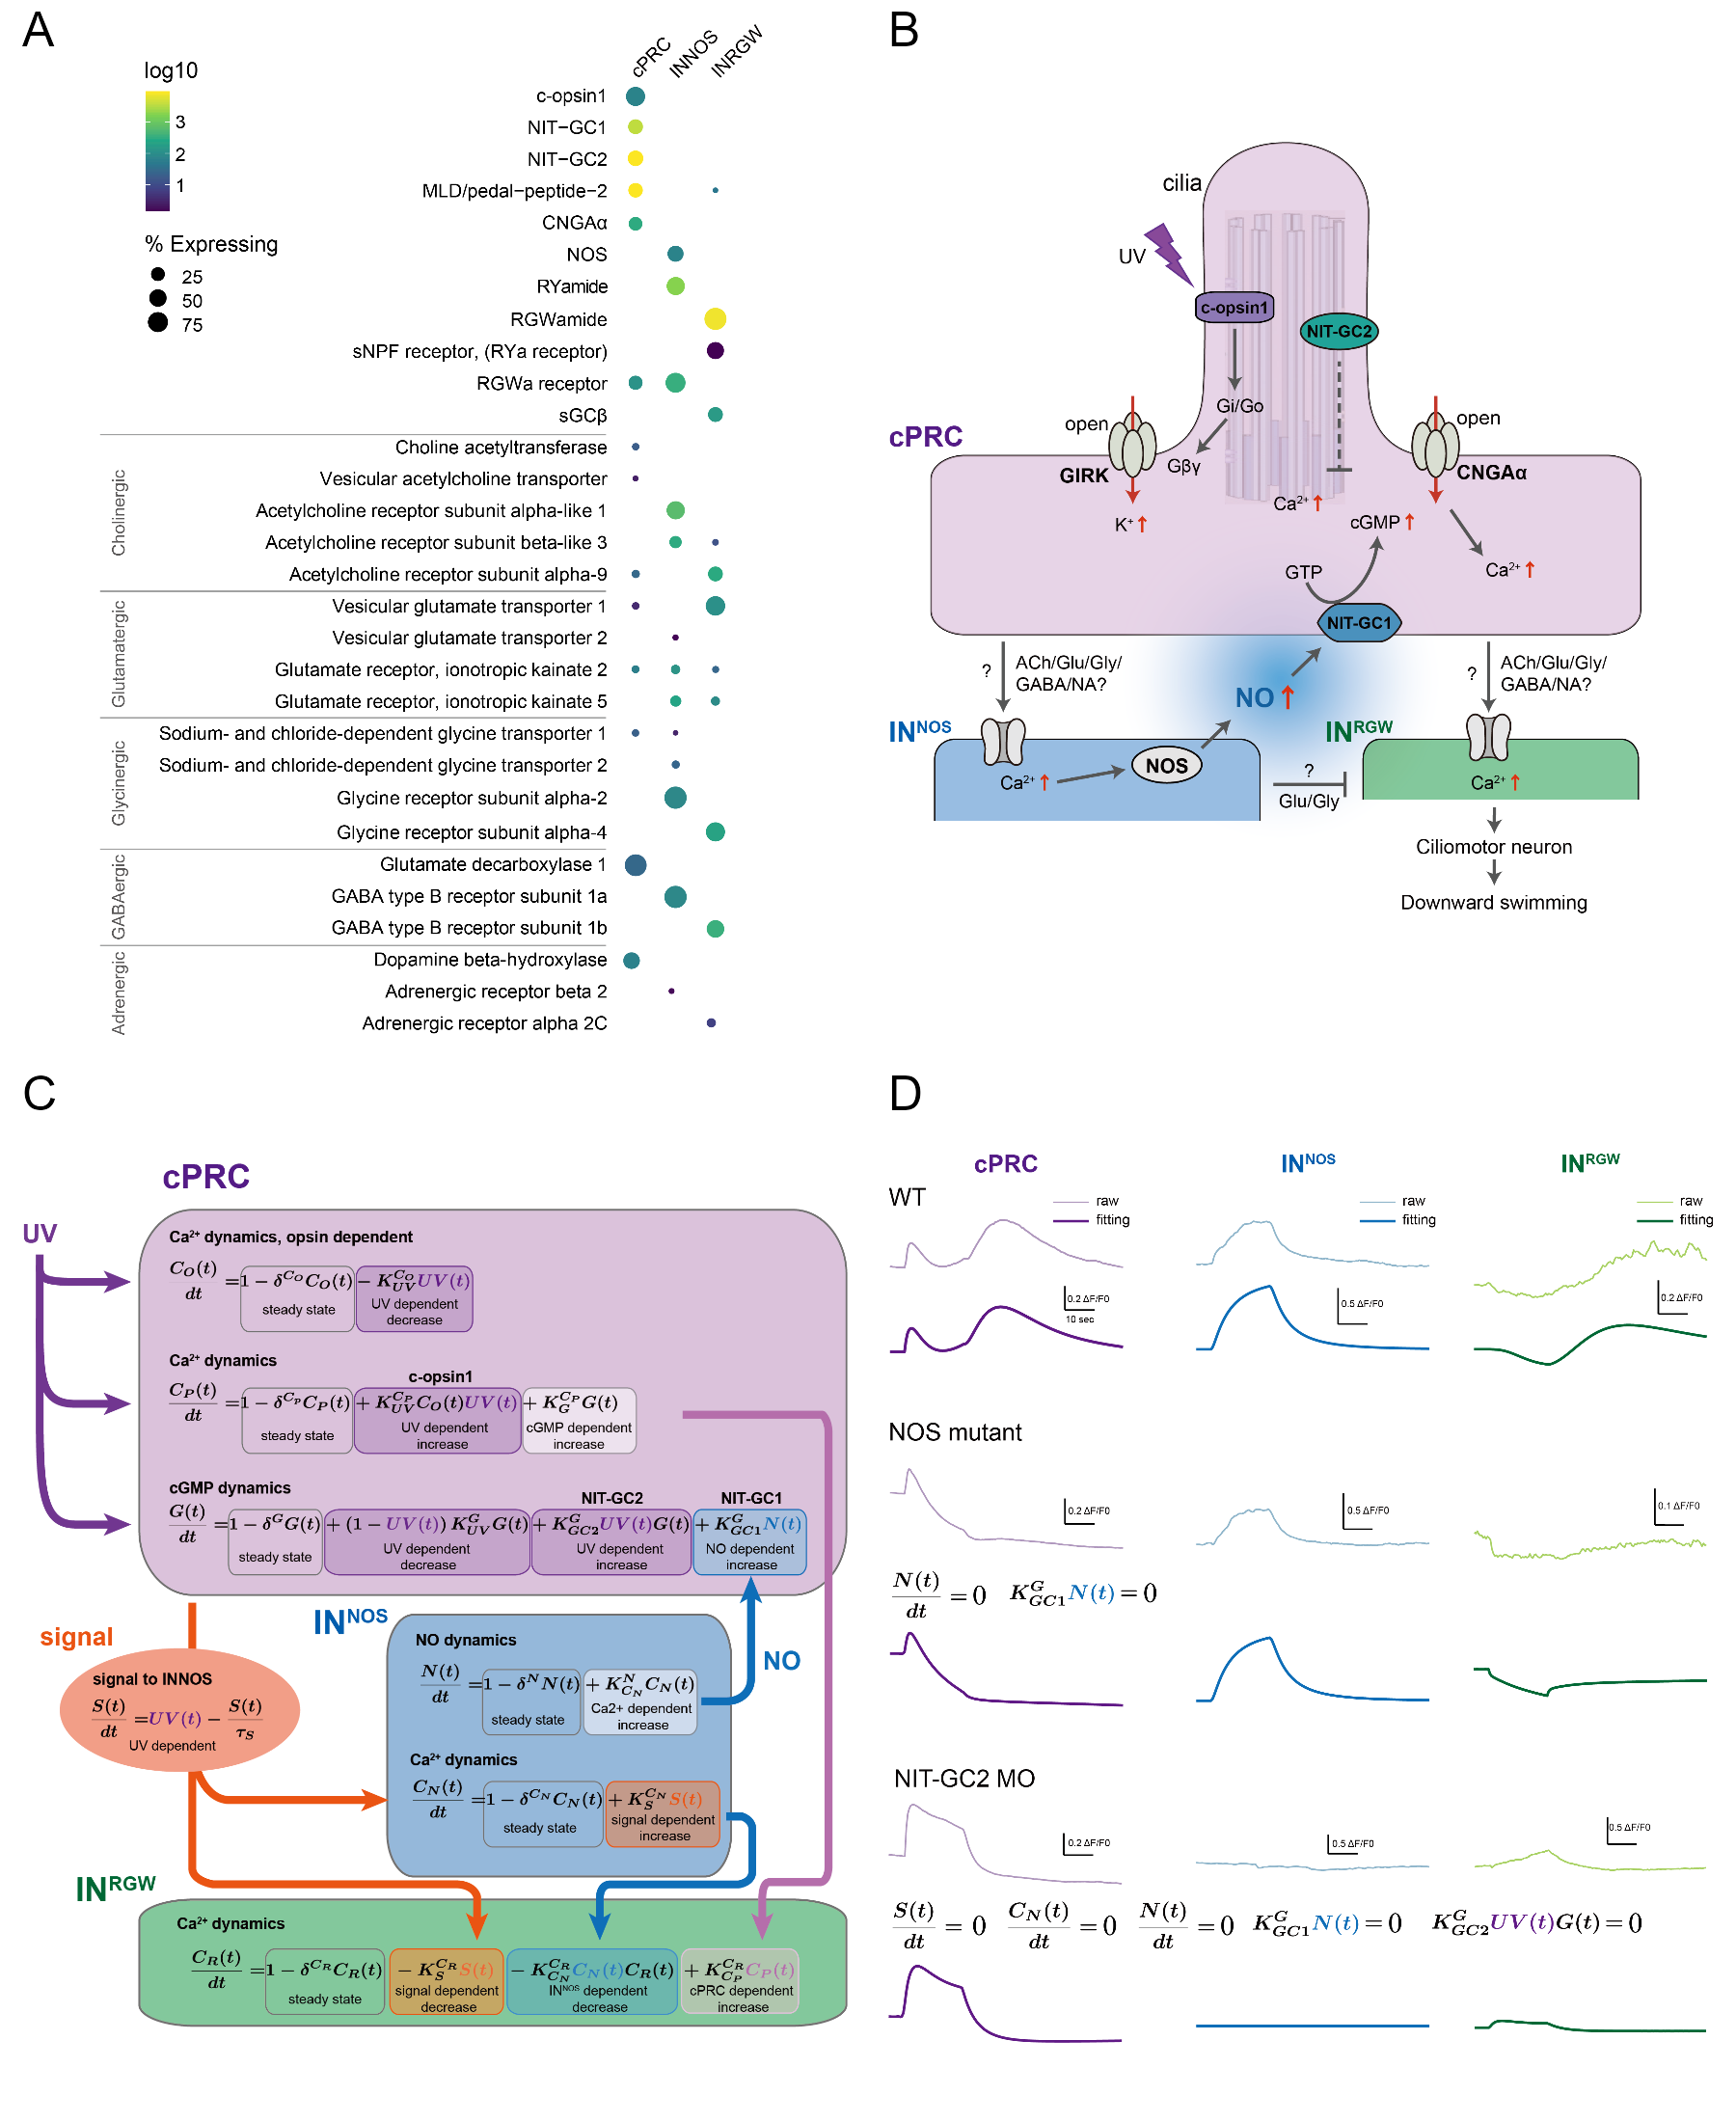
\includegraphics[width=25in]{figures/Fig6} \caption{**Figure 6. Mathematical modelling of cPRC circuit dynamics during UV stimulation and potential signalling mechanisms.**  **(A)** Diagram for **(B)** **(C)** Dot plot of genes (columns) expressed in three types of cells (rows) in the cPRC circuit using single cell RNA-Seq. The size of the dots is expressed in proportion to the percentage of cells expressing that gene relative to all cells. The colours represent the normal logarithm of the number of transcripts in the cells expressing the gene. **(D)** Schematic diagram of the signalling pathway of the cPRC circuit, focusing on the NO feedback.}\label{fig:unnamed-chunk-6}
\end{figure}

\hypertarget{discussion}{%
\subsection{Discussion}\label{discussion}}

Our work revealed an essential role for NO-mediated signalling in
driving UV/violet avoidance behaviour in larval \emph{Platynereis}. NO,
produced by postsynaptic INNOS interneurons, signals retrogradely to
presynaptic cPRCs via NIT-GC1 leading to delayed and sustained cPRC
activation. This late-phase activation of the photoreceptors drives
circuit output through projection interneurons and ciliomotor neurons.
In the cPRC circuit, synaptic connectivity alone is thus not sufficient
to account for circuit dynamics and behavioural change, as documented in
other circuits (Bargmann and Marder, 2013; Imambocus et al., 2022).

\textbf{Localised NO signalling in the neurosecretory plexus}

NO is a free radical with a millisecond-to-second half life and thus a
limited signalling range. In neuronal signalling, NOS is often localized
to neurites (Kuntz et al., 2017) at close proximity to sGC at synapses
(Burette et al., 2002; Garthwaite, 2015). In the cPRC circuit, NOS is
localised to the dendritic compartment of INNOS cells where also cPRC
postsynaptic sites occur. NIT-GC1, the target of NO signalling is
localised to cPRC projections. NO-mediated retrograde signalling thus
likely occurs in the neurosecretory plexus where NOS- and
NIT-GC1-containing projections are in close proximity and where we
detected NO production following UV stimulation. In contrast, INNOS to
INRGWa synapses occur outside the neurosecretory plexus in the ventral
brain neuropil.

Compartmentalised signalling also occurs in peptidergic modulatory
systems and can enable selective network activity during specific
behaviours. In the UV-avoidance circuit of \emph{Drosophila} larvae, a
peptidergic hub neuron Dp7 links UV-sensory neurons (v'td2) and motor
circuits. Dp7 expresses an an insulin-like peptide Ilp7 that is required
for acute and sustained UV avoidance. Ilp7 signalling occurs at a
functionally and morphologically distinct dendritic compartment of Dp7,
segregated from other sensory-motor pathways involving Dp7 (Imambocus et
al., 2022).

\textbf{Functional diversity of NIT-GCs}

NO signalling is commonly mediated by sGCs. We identified 12 sGCs in
\emph{Platynereis}, but none of these is expressed in the cPRC based on
the available scRNAseq data. Instead, we identified an unconventional
cPRC-expressed NIT-domain containing GC, NIT-GC1 as the mediator of NO
retrograde signalling. In an in vitro assay, we could show that NIT-GC1
can produce cGMP following the addition of an NO donor and that this
activity requires the NIT domain.

NIT domains were first identified in bacteria and animal NIT-GCs have
only recently been reported (Moroz et al., 2020; Shu et al., 2003).
Bacterial NIT domains regulate cellular functions in response to changes
in extracellular and intracellular nitrate and nitrite concentrations
(Camargo et al., 2007). NO is readily converted to nitrate and nitrite
(Garthwaite, 2015; Möller et al., 2019; Santos et al., 2011) and these
molecules accumulate in placozoans and cnidarians in cells and tissues
with high NOS activity (Moroz et al., 2020, 2004). NIT domains in
NIT-GCs may also sense nitrate and nitrite, as in bacteria, a
possibility we cannot rule out based on our cellular assays with
NIT-GC1. If different NIT-GCs have different sensitivities to NO,
nitrite and nitrate, then a range of activation timings may be possible
due to the different half-lives of these molecules (Lundberg et al.,
2011).

NIT-GC1 and NIT-GC2 showed specific cellular co-expression but very
different subcellular localisation and function. In \emph{Platynereis},
we identified 15 NIT-GCs, suggesting a wide range of functions.
Differences in subcellular localisation and biochemical function thus
seem to also contribute to the diversity of NIT-GC functions in addition
to differences in expression.

\textbf{Mechanism of phototransduction and neurotransmission in the cPRC
circuit}

Based on our data herein and previous work we can now propose a more
detailed model of cPRC phototransduction and neurotransmission. The
cPRCs have high basal Ca2+ and respond to UV/violet light dependent on
c-opsin1 (Verasztó et al., 2018). c-opsin1 forms a bistable photopigment
and signals through Gi/oα and Gβγ (Tsukamoto et al., 2017; Tsukamoto and
Kubo, 2023; Veedin Rajan et al., 2021). In heterologous systems, the Gβγ
subunits released following c-opsin1 activation open GIRK channels
inducing K+ efflux (hyperpolarisation) (Tsukamoto et al., 2017;
Tsukamoto and Kubo, 2023) and close voltage-gated Ca2+ channels, thereby
reducing intracellular calcium levels (Tsukamoto and Kubo, 2023). A GIRK
channel is also expressed in the cPRCs (Figure 6A). The pathway for the
first rapid cPRC activation phase following UV/violet stimulus is not
known but may involve the activation of a CNGα channel expressed in the
cPRCs (Tosches et al., 2014). For the second inhibitory phase of
phototransduction, we identified a key requirement for ciliary-localised
NIT-GC2. The mechanisms may involve c-opsin1-dependent inhibition of
tonic NIT-GC2 activity and the reduction of ciliary cGMP.

NIT-GC2-dependent signalling is required for the feedforward activation
of the INNOS cells through an unknown transmitter. The activation of
INNOS leads to NOS activation and NO release, potentially through a
canonical Ca2+-calmodulin pathway. Our model predicts feedforward
inhibiton from INNOS to INRGWa, possibly mediated by glycin
transmission. NO released by INNOS neurites activates NIT-GC1 in cPRC
projections that could lead to cGMP production and the opening of CNGAα.
This late-phase cPRC activation is not directly dependent on the
UV/violet signal and can happen post-stimulus. The late-phase cPRC
activation leads to INRGWa activation via an unknown transmitter that is
likely different from the one acting on INNOS.

In addition, the cPRC circuit expresses several neuropeptides and their
receptors, suggesting further neuromodulatory signals. For example,
INRGWa express the proneuropeptide RGWamide and cPRCs and INNOS express
its receptor, suggesting retrograde peptidergic signalling in the
circuit.

We have recently shown that the cPRC circuit also mediates responses to
hydrostatic pressure via the same motor system involving Ser-h1 and the
prototroch ciliary band. Increased pressure induces cPRC activation and
a circuit output that is inverted relative to UV-induced activation.
Consequently, ciliary beating increases and the larvae swim upwards. The
effect of pressure on cilia requires synaptic transmission by the
serotonergic Ser-h1 neurons (Bezares-Calderón et al., 2023).

Pressure-induced Ca2+ transients in cPRCs lack an inhibitory phase and
late activation and resemble UV responses in NIT-GC2 morphants
(Bezares-Calderón et al., 2023). This indicates that the differentiation
of sensory cues by the multisensory cPRCs occurs already at the level of
sensory signal transduction. The different signalling pathways then
likely result in the differential release of transmitters and modulators
that are decoded by the postsynaptic interneuron circuit. The complex
transmitter phenotype of cPRCs could underlie such differential signal
processing.

\textbf{Nitric oxide confers short-term memory to circuit activity}

Retrograde signalling by NO from INNOS to cPRC leads to the sustained
activation of cPRCs and postsynaptic neurons even after the end of
stimulation. This activated state is maintained for several tens of
second. NO signalling thus induces a transient circuit state or
short-term memory trace in the \emph{Platynereis} larval brain. Because
of the short life time of NO, this molecule may be well suited to encode
transient memory traces (Kuntz et al., 2017).

In the ellipsoid body of the \emph{Drosophila} central brain, NO
signalling has a similar function. Here, NOS is specifically expressed
in the R3 ring neurons and is required for the short-term
(\textasciitilde4 sec) visual memory of objects (Kuntz et al., 2017). NO
is produced in the axons of R3 neurons and acts directly on sGC in the
same axons. This autocrine signal leads to a CNG-dependent temporary
increase in calcium levels, carrying the working memory trace (Kuntz et
al., 2017).

In the \emph{Platynereis} circuit, our mathematical model indicates that
the onset, magnitude and duration of the NO-dependent signal depends on
the intensity and duration of the UV/violet stimulus. This suggests that
the NO-dependent memory trace also encodes the magnitude and duration of
the stimulus.

During UV avoidance in the planarian \emph{Schmidtea mediterranea},
neuropeptide signalling has a similar integratory function. Planarians
exposed to UV light for \textgreater30 sec remain active for extended
periods (several minutes) post-stimulation (Bray et al., 2023). If
neuropeptide signalling is defective, animals can still respond to UV
light, but do not maintain a latent memory state and do not display
increased post-stimulus activity.

\textbf{The possible mechanism of UV-induced downward swimming}

Non-directional UV/violet light induces downward swimming head down in
\emph{Platynereis} larvae (Verasztó et al., 2018). Since stimulus
direction is not relevant, swimming direction must be determined by
gravity.

Connectome reconstruction and whole-body cell annotation in the
three-day-old \emph{Platynereis} larva has not revealed any balancer
organ to sense orientation in the gravity field (Bezares-Calderón et
al., 2019; Verasztó et al., 2020). It follows that body orientation must
be determined by physical parameters including the buoyancy, centre of
mass and shape of the larva as well as differential ciliary activity.
Except for ciliary activity, all these parameters are likely invariant
during the UV response. Our data suggest the UV-dependent inhibition of
prototroch ciliary beating via Ser-h1 inhibition and MC activation
(Verasztó et al., 2017).

We hypothesise that the differential beating of prototroch versus trunk
cilia causes a head-up or head-down orientation due to physics alone.
During the UV response, prototroch cilia beat slower than trunk cilia,
resulting in a head-down stable state (`rear-wheel drive'). In contrast,
during the pressure response prototroch cilia beat faster than trunk
cilia (Bezares-Calderón et al., 2023), leading to a head-up orientation
(`front-wheel drive'). Testing this hypothesis will require biophysical
experiments and mathematical modelling.

\hypertarget{uv-avoidance-circuits-of-extraocular-photoreceptors}{%
\subsection{UV-avoidance circuits of extraocular
photoreceptors}\label{uv-avoidance-circuits-of-extraocular-photoreceptors}}

Animals evolved distinct photosensory systems coupled to non-overlapping
circuits and guiding unique behavioural responses. These sensory systems
can employ different opsin molecules and be tuned to different
wavelengths of light. The avoidance of noxious UV/violet light is often
mediated by extraocular photoreceptors and their circuits, distinct from
the pigmented visual eyes. These two types of systems co-exist in
\emph{Platynereis} where the pigmented eyes and eyespots guide
phototaxis with a maximum sensitivity to cyan light (\textasciitilde500
nm) (Randel et al., 2014; Verasztó et al., 2018). Planarians also have
pigmented visual eyes mediating phototaxis to cyan light and peripheral
extraocular photoreceptors mediating UV avoidance behaviour (Shettigar
et al., 2021). \emph{Drosophila} larvae have cerebral eyes called
Bolwig's organs involved in phototaxis (Kane et al., 2013) and several
types of extraocular UV-sensory cells that tile the body wall and
mediate UV avoidance (Imambocus et al., 2022).

One common feature of UV-avoidance circuits is their sustained
post-stimulus activation following UV exposure. This can involve
peptidergic signals as in planaria and maggots (Bray et al., 2023;
Imambocus et al., 2022) or NO as in \emph{Platynereis}. Volume
transmission is well suited to integrate light exposure and maintain an
internal state following noxious stimulation. The amount of modulator
released can scale with stimulus intensity or duration and maintain an
altered circuit state due to the slower decay of the diffusive signals
relative to synaptic transmission.

We have revealed how NO shapes dynamics in a fully-mapped sensory-motor
UV avoidance circuit. We identified an unconventional GC as the NO
receptor in \emph{Platynereis} and measured circuit activity in
different genetic backgrounds. Finally, we could link circuit activity
to light-avoidance behaviour. The richly modulated multi-transmitter
cPRC circuit will serve as a fertile ground for future studies on how
neuromodulators shape activity and behaviour.

\hypertarget{key-resources-table}{%
\subsection{Key resources table}\label{key-resources-table}}

Reagent type (species)

Designation

Source or reference

Identifiers

Additional information

Strain (Platynereis dumerilii)

NOSΔ11/Δ11~knockout

~This paper

NA

~Knockout generated by CRISPR/Cas-9-induced gene editing

Strain (Platynereis dumerilii)

NOSΔ23/Δ23~knockout

~This paper

NA

~Knockout generated by CRISPR/Cas-9-induced gene editing

Strain (Platynereis dumerilii)

NOSΔ11/Δ23~knockout

~This paper

NA

~Knockout generated by CRISPR/Cas-9-induced gene editing

Cell line (Cercopithecus aethiops)

COS-7 cell

NA

RRID:CVCL\_0224

Angio-proteomie (CAT no. cAP-0203)??

Biological sample (Platynereis dumerilii)

Wild type Tübingen strain

Other

NCBITaxon:6359

Jékely lab strain (Tübingen, Exeter)

Gene (Platynereis dumerilii)

NOS

This paper

GenBank\_Acc\#:

NA

Gene (Platynereis dumerilii)

NIT-GC1

This paper

GenBank\_Acc\#:

NA

Gene (Platynereis dumerilii)

NIT-GC2

This paper

GenBank\_Acc\#:

NA

NOS: Nitric\_Oxide\_Synthase

To amplify Promoter \& Regulatory region

Fwd

NOSProm2ndF0.6BamHI

AGGGATCCCCCAATGCTTTAGCAGTCAGAGGAG

NOS: Nitric\_Oxide\_Synthase

To amplify Promoter \& Regulatory region

Rev

GeR1ASCI

AAGGCGCGCCCCACCACCACCTTTGATATCCATGATGCTCACTTCGC

NOS: Nitric\_Oxide\_Synthase

Mutation Check on Exon3

Fwd

Exon3 Sequence F-27bp

GGTTCATTGGTTTCGATAACATTGCGG

NOS: Nitric\_Oxide\_Synthase

Mutation Check on Exon3

Rev

Exon3 Sequence R-27bp

CAGAGTCGATCAGTCTGCATATCTCCA

NOS: Nitric\_Oxide\_Synthase

Sequencing primer for Exon3 mutation check PCR product

Fwd

Exon3 Sequence F-2

GGTGCTCTCCCGGGTACACAA

RNA

sgRNA

NA

NA

5'-TAGGGCAATACTGGCTCCACTC-3'

RNA

sgRNA

NA

NA

5'-AAACGAGTGGAGCCAGTATTGC-3'

RNA

pUC57-T7-RPP2-hSpCas9- HA-2XNLS-GFP

NA

plasmid

Bezares-Calderón et al., 2018

Antibody

Monoclonal Anti-Tubulin, Acetylated antibody

Sigma-Aldrich

Cat\#:T6793, RRID:AB\_477585

NA

Antibody

HA-Tag (C29F4), Rabbit mAb

Cell Signaling Technology

Cat\#:3724P

NA

NIT-GC1 polychronal antibodies

CYWLLGRKERRPKRRL-amide

This paper

rabbit

Altabioscience

NIT-GC2 polychronal antibodies

CTEGSTKEGKKEGQ-amide

This paper

rabbit

Altabioscience

NOS polychronal antibodies

CKPSYELQDPWKTYIWRKD-amide

This paper

Rat

Altabioscience

Antibody

RYamide neuropeptide antibodies

CRY-amide

rabbit

Conzelmann and Jékely, 2012

Antibody

RGWamide neuropeptide antibodies

CGW-amide

rabbit

Conzelmann and Jékely, 2012

Antibody

F(ab')2-Goat anti-Rabbit IgG (H+L) Cross-Adsorbed Secondary Antibody,
Alexa Fluor™ 546

Invitrogen

Catalog \# A-11071

NA

Antibody

Goat anti-Rat IgG (H+L) Highly Cross-Adsorbed Secondary Antibody, Alexa
Fluor™ Plus 594

Invitrogen

Catalog \# A48264

NA

Antibody

F(ab')2-Goat anti-Mouse IgG (H+L) Cross-Adsorbed Secondary Antibody,
Alexa Fluor™ 647

Invitrogen

Catalog \# A-21237

NA

Recombinant DNA reagent

NIT-GC1 full

comp411593\_c0\_seq1\_309\_F

NA

GGTTGAATAATGACAAGCAAGGAGA

Recombinant DNA reagent

NIT-GC1 full

comp411593\_c0\_seq1\_2717\_R

NA

GTGCTATCATTTCCAGGTAAATACCC

Recombinant DNA reagent

NIT-GC2 full

Contig2280\_66\_F

NA

AATATCTAGCGAAGGAGAACACCTCTCTTC

Recombinant DNA reagent

NIT-GC2 full

Contig2280\_2763\_R

NA

ATGGCCAGTAATAAACCATCAGTGGTTC

Recombinant DNA reagent

pcDNA3.1(+) vector

Invitrogen

Catalog Number: V79020

NA

Recombinant DNA reagent

Inverse PCR for the insert region of pcDNA3.1(+)

pcDNA3.1(+)\_inv\_NheI\_fwd

NA

CGTTTAAACTTAAGCTTGGTACCGAG

Recombinant DNA reagent

Inverse PCR for the insert region of pcDNA3.1(+)

pcDNA3.1(+)\_inv\_NheI\_rev

NA

CCAGCTTGGGTCTCCCTATAGT

Recombinant DNA reagent

kozak-NITGC2-T2A-Green cGull

NITGC-T2A-fwd

NA

TATAGGGAGACCCAAGCTGGGCCACCATGACCCAGATG

Recombinant DNA reagent

kozak-NITGC2-T2A-Green cGull

NITGC-T2A-rev1

NA

GCATGTTAGAAGACTTCCTCTGCCCTCATAATCAAACCCCTCTCT

Recombinant DNA reagent

kozak-NITGC2-T2A-Green cGull

NITGC-T2A-rev2

NA

AGGGCCGGGATTCTCCTCCACGTCACCGCATGTTAGAAGACTTCC

Recombinant DNA reagent

kozak-NITGC2-T2A-Green cGull

NITGC-T2A-rev3

NA

TGCTCACCATAGGGCCGGGATTCTCCTC

Recombinant DNA reagent

kozak-NITGC2-T2A-Green cGull

cGull-fwd

NA

TCCCGGCCCTATGGTGAGCAAGGGCGAG

Recombinant DNA reagent

kozak-NITGC2-T2A-Green cGull

cGull-rev

NA

ACCAAGCTTAAGTTTAAACGTTACTTGTACAGCTCGTCCATG

Recombinant DNA reagent

Green cGull-T2A-NITGC2 \& NITGC2-T2A-Green cGull

NITGC2\_seq\_743\_fwd

NA

AGCCATCTACGAGTGGTA

Recombinant DNA reagent

Green cGull-T2A-NITGC2 \& NITGC2-T2A-Green cGull

cGull\_seq\_385\_rev

NA

TGCCCTTCAGCTCGATG

Recombinant DNA reagent

Green cGull-T2A-NITGC2 \& NITGC2-T2A-Green cGull

NITGC2\_seq\_743\_rev

NA

TGACTGACGAACCCTCC

Recombinant DNA reagent

Green cGull-T2A-NITGC2 \& NITGC2-T2A-Green cGull

NITGC2\_seq\_394\_fwd

NA

AGATATCTTGAAACGGACGA

Recombinant DNA reagent

kozak-NIT1(seq)-T2A-Green cGull

2A-cGull\_invF\_L1

NA

TGACGTGGAGGAGAATCCCGGCCCTATGGTGAGCAAGGGCGAGGAGCTGT

Recombinant DNA reagent

kozak-NIT1(seq)-T2A-Green cGull

2A-cGull\_invF\_L2

NA

GCAGAGGAAGTCTTCTAACATGCGGTGACGTGGAGGAGAATCCCGGCCCT

Recombinant DNA reagent

kozak-NIT1(seq)-T2A-Green cGull

2A-cGull\_invR\_L

NA

TCCTTGCTTGTCATGGTGGCCCAGCTTGGGTCTCCCTATAGTGAGTCGTA

Recombinant DNA reagent

kozak-NIT1(seq)-T2A-Green cGull

NIT1-2A\_F\_L

NA

GAGACCCAAGCTGGGCCACCATGACAAGCAAGGAGATGCCTGTACTCATG

Recombinant DNA reagent

kozak-NIT1(seq)-T2A-Green cGull

NIT1-2A\_R\_L

NA

TGTTAGAAGACTTCCTCTGCCCTCTATGACTTTTTCTATGCTTTCTTCGG

Recombinant DNA reagent

kozak-NIT1(seq)-T2A-Green cGull

NIT1seq\_remo\_invF2

NA

AGCGTGGAGGTGGGCCTAGACGAAAGAGCTGAAAA

Recombinant DNA reagent

kozak-NIT1(seq)-T2A-Green cGull

NIT1seq\_remo\_invR2

NA

AGCTCTTTCGTCTAGGCCCACCTCCACGCTGAATA

Recombinant DNA reagent

kozak-NIT1(seq)-T2A-Green cGull

NIT1seq\_remo\_F2

NA

GCCGGTCTTGTCGATCAGGATGATCTGGAC

Recombinant DNA reagent

kozak-NIT1(seq)-T2A-Green cGull

NIT1seq\_remo\_R2

NA

GTCCAGATCATCCTGATCGACAAGACCGGC

Recombinant DNA reagent

pUC57-NOSp::Palmi-3xHA-tdTomato (plasmid)

This paper

NA

Promoter construct: injected at 250 ng/μl

Recombinant DNA reagent

pUC57-T7-RPP2-tdTomato-P2A-GCaMP6 (plasmid)

This paper

NA

Used for generating tdTomato-P2A-GCaMP6s mRNA

Plasmid

Green cGull

Addgene

Plasmid \#86867

NA

HCR

NOS

Integrated DNA Technologies

NA

NA

HCR

NIT-GC1

Integrated DNA Technologies

NA

NA

HCR

NIT-GC2

Integrated DNA Technologies

NA

NA

HCR

RYa-pNP (GenBank accession: JF811330.1)

Integrated DNA Technologies

NA

NA

HCR

c-opsin1 (GenBank accession: AY692353.1)

Integrated DNA Technologies

NA

NA

HCR

MLD/pedal2-pNP (GenBank accession: KF515945.1)

Integrated DNA Technologies

NA

NA

HCR

CNGAα (GenBank accession: KM199644.1)

Integrated DNA Technologies

NA

NA

fluorescently labeled hairpins

B2-647

Molecular Technologies

NA

NA

fluorescently labeled hairpins

B3-546

Molecular Technologies

NA

NA

morpholino

NIT-GC1 MO1

Gene-Tools, LLC

NA

TGCTTGTCATTATTCAACCAGCAAA

morpholino

NIT-GC1 MO2

Gene-Tools, LLC

NA

TTCAATTAAACCCTCCAGGTTGCTG

morpholino

NIT-GC2 MO1

Gene-Tools, LLC

NA

AAATGAAGAGAGGTGTTCTCCTTCG

morpholino

NIT-GC2 MO2

Gene-Tools, LLC

NA

ATATTCATTATGTGAAGAACTTCCA

plasmid for mRNA synthase (GCaMP6s)

BamHI-T7::RPP2(5UTR)-GCaMP6s(AscI-AgeI)-polyA\_KpnI\_c1

NA

Plasmid

Bezares-Calderón et al., 2018

plasmid for mRNA synthase (RGECO1a)

PUC57-T7-PduRPP2(5UTR)-jRGECO1a

NA

Plasmid

Bezares-Calderón et al., 2018

Chemical compound, drug

SNAP

Sigma-Aldrich

Cat\#:M9020

500 μM

Chemical compound, drug

L-NAME

Sigma-Aldrich

Cat\#:M9021

501 μM

Commercial assay or kit

Phusion Human Specimen Direct PCR Kit

Thermofisher

NA

NA

Commercial assay or kit

mMESSAGE mMACHINE Sp6 kit

Thermofisher

NA

NA

Software, algorithm

Golden Gate TAL

Addgene 1000000024

NA

NA

Software, algorithm

Effector Kit 2.0, Fiji perl and Fiji scripts for tracking

PMID: 22743772, \url{https://github.com/JekelyLab/Veraszto_et_al_2018}

RRID:SCR\_002285

0000d2a

Commercial assay or kit

QuickExtract

Epicentre,US

Cat\#:QE09050

NA

Commercial assay or kit

MEGAshortscript T7 Transcription Kit

Ambion, ThermoFisher Scientific

Cat\#:AM1354

NA

Commercial assay or kit

mMESSAGE mMACHINE T7 ULTRA Transcription Kit

Ambion, ThermoFisher Scientific

Cat\#:AM1345

NA

Commercial assay or kit

MEGAclear Transcription Clean-Up Kit

Ambion, ThermoFisher Scientific

Cat\#:AM1908

NA

Software, algorithm

Fiji

NIH

RRID:SCR\_002285

NA

Software, algorithm

R Project for Statistical Computing

R Foundation

RRID:SCR\_001905

NA

Software, algorithm

Imaris Version 8.0.0

Bitplane, UK.

RRID:SCR\_007370

NA

Software, algorithm

CATMAID

\url{DOI:10.1093/bioinformatics/btp266}

RRID:SCR\_006278

NA

Software, algorithm

PhyML

\url{DOI:10.1093/sysbio/syq010}

RRID:SCR\_014629

NA

Software, algorithm

Gblocks

\url{DOI:10.1080/10635150701472100}

RRID:SCR\_015945

NA

\hypertarget{materials-and-methods}{%
\subsection{Materials and Methods}\label{materials-and-methods}}

\textbf{CRISPR-Cas9 Design and Microinjection}

Before designing the small guide RNA (sgRNA) for the sgRNA:Cas9
nuclease, splice sites and polymorphic sites in our laboratory culture
were identified to avoid them. The sgRNA targeted the third exon of
Platynereis dumerilii NOS (target site: 5'-GGGCAATACTGGCTCCACTC-3'). The
sgRNA was assembled from two annealed oligonucleotides
(5'-TAGGGCAATACTGGCTCCACTC-3', 5'-AAACGAGTGGAGCCAGTATTGC-3') forming
overhangs for cloning into a BsaI site of the plasmid pDR27456 (Hwang et
al.~2013)(42250, Addgene), which contains next to the BsaI site a
tracrRNA sequence. The plasmid was then used to PCR amplify DNA
(primers: T7, 5'-AAAAGCACCGACTCGGTGCC-3') for synthesizing the sgRNA.
The DNA was purified with the QIAquick PCR Purification Kit (Qiagen).
From the DNA, the sgRNA was synthesized with the MEGAshortscript Kit
(Thermo Fisher Scientific) and was purified with the MEGAclear Kit
(Thermo Fisher Scientific). Cas9-mRNA was transcribed, capped, and
polyA-tailed with the mMessage mMachine Kit and the Poly(A) Tailing Kit
(both Thermo Fisher Scientific) from a plasmid (pUC57-T7-RPP2-Cas9)
containing the Cas9 ORF fused to 169 base pair 5' UTR from the
Platynereis dumerilii 60S acidic ribosomal protein P2. The sgRNA (18
ng/ml) and the Cas9-mRNA (180 ng/µl) were coinjected into fertilized
eggs of Platynereis dumerilii wild-type parents according to an
established injection procedure (Conzelmann et al., 2013). The eggs were
kept at 18°C for 45 min before injection and were injected at 14.5°C.
The injected individuals were kept at 18°C for 5 to 8 days in 6-well-
plates (Nunc multidish no. 150239, Thermo Scientific) and then cultured
at 22°C until sexual maturity. The mature worms were crossed to
wild-type worms and the progeny was genotyped, resulting in two founder
lines, which were bred to homozygosity.

\textbf{NOS sequencing and genotyping}

For genotyping of the NOS locus, genomic DNA was isolated from single
larvae, groups of 6-20 larvae, or from the tails of adult worms. The DNA
was amplified by PCR (primers: 5'-GGTTCATTGGTTTCGATAACATTGCGG-3',
5'-CAGAGTCGATCAGTCTGCATATCTCCA-3') with the dilution protocol of the
Phusion Human Specimen Direct PCR Kit (Thermo Scientific). The PCR
product was sequenced directly with a nested sequencing primer
(5'-GGTGCTCTCCCGGGTACACAA-3'). A mixture of wild-type and deletion
alleles in a sample gave double peaks in the sequencing chromatograms,
with the relative height of the double peaks reflecting the relative
allele ratio in the sample.

\textbf{Vertical column setup for measuring photoresponses}

Photoresponses of larvae of different ages were assayed in a vertical
Plexiglas column (31 mm x 10 mm x 160 mm water height). The column was
illuminated from top with light from a monochromator (Polychrome II,
Till Photonics). The monochromator was controlled by AxioVision 4.8.2.0
(Carl Zeiss MicroImaging GmbH) via analog voltage. The light passed a
collimator lens (LAG-65.0-53.0-C with MgF2 Coating, CVI Melles Griot)
before entering the column. The column was illuminated from both sides
with light-emitting diodes (LEDs). The LEDs on each side were grouped
into two strips. One strip contained UV (395 nm) LEDs (SMB1W-395,
Roithner Lasertechnik) and the other infrared (810 nm) LEDs
(SMB1W-810NR-I, Roithner Lasertechnik). The UV LEDs were run at 4 V to
stimulate the larvae in the column from the side. The infrared LEDs were
run at 8 V (overvoltage) to illuminate the larvae for the camera (DMK
22BUC03, The Imaging Source), which recorded videos at 15 frames per
second and was controlled by IC Capture (The Imaging Source).

\textbf{Comparing behavior of wildtype and NOS-knockout 3-day-old
larvae}

To compare the behavior of wildtype and NOS-knockout larvae at 3 days in
the vertical column, the larvae were mixed and left in the dark for 5
min. The larvae were treated with NOS inhibitors for pharmacology. The
NOS inhibitors were L-NAME. The larvae were treated with different
concentrations in adjacent columns. The concentrations for the NOS
inhibitors were control, 1 mM, 0.1 mM. The larvae were recorded for 1
min in the dark followed by exposure to collimated cyan (480 nm) light
from the top of the column for 2 min, then 2 min darkness, and finally
collimated UV (395 nm) light from the top of the column for 2 min.
Stimulus light was provided by the monochromator (Polychrome II, Till
Photonics). Scripts are available at
\url{https://github.com/JekelyLab/NOS}.

\textbf{NOS Identification and Phylogenetic Analysis}

To identify NOS, we obtained a ``seed'' database of oxygenase domain in
Pfam database, PF02898. From these sequences, we produced a Hidden
Markov Model (HMM) and used this to mine the 47 metazoan species, 2
choanoflagellate species and 2 filasterea species investigated. HMM
models were run in HMMR3 with an e-value of 1e−15. We ran CD-Hit (Fu et
al., 2012) to eliminate redundant sequences (at a 80\% threshold). We
aligned the sequences with MAFFT version 7, with the iterative
refinement method E-INS-i. Alignments were trimmed with TrimAl in
gappy-out mode (Capella-Gutierrez et al., 2009). To calculate
maximum-likelihood trees, we used IQ-tree2 with the LG+G4 model. To
calculate branch support, we ran 1,000 replicates with the aLRT-SH-like
and aBayes methods (Minh et al., 2020). The sequences used for the
phylogenetic analysis are available in \textbf{Supplementary File 1},
the trimmed alignment is available in \textbf{Supplementary File 2} and
the pre-trimmed data in \textbf{Supplementary file 3}.

\textbf{NIT-GC Identification and Phylogenetic Analysis}

To identify NIT-GCs, we obtained a ``seed'' database of Adenylate and
Guanylate cyclase catalytic domain in Pfam database, PF00211. From these
sequences, we produced a Hidden Markov Model (HMM) and used this to mine
the 45 metazoan species, 2 choanoflagellate species and 2 filasterea
species investigated. HMM models were run in HMMR3 with an e-value of
1e−15. We ran CD-Hit (Fu et al., 2012) to eliminate redundant sequences
(at a 80\% threshold). To identify clusters, we used the
convex-clustering option with 100 jack-knife replicates. The NIT-GCs are
extremely well conserved in membrane-bound guanylate cyclases and form
an easily recognizable cluster. To analyze the phylogeny of NIT-GCs, the
cluster containing these GCs together with membrane-bound guanylate
cyclases were parsed and used for tree building. We aligned the
sequences with MAFFT version 7, with the iterative refinement method
E-INS-i. Alignments were trimmed with TrimAl in gappy-out mode
(Capella-Gutierrez et al., 2009). To calculate maximum-likelihood trees,
we used IQ-tree2 with the LG+G4 model. To calculate branch support, we
ran 1,000 replicates with the aLRT-SH-like and aBayes methods (Minh et
al., 2020). The sequences used for the phylogenetic analysis are
available in \textbf{Supplementary File 1}, the trimmed alignment is
available in \textbf{Supplementary File 2} and the pre-trimmed data in
\textbf{Supplementary file 3}.

\textbf{Single-cell analysis}

We used Achim et al.~for the single-cell data (Achim et al., 2015). In
Williams et al., they used 107 cells as neurons by removing duplicates
from Achim et al.~single-cell data, so we used those cells (Williams et
al., 2017). Since the raw data were read count data, we normalized them
to TPM using Python. After that we converted them to log10. From the sum
of the expression levels in 107 cells for each gene, We calculated the
percentage in each cell. For each cell, we identified them with marker
genes. After created the data in Python, plotted it using R dot plots.
RPKM calculates the total number of reads per million bp and then
divides by the length of each gene, so it is not possible to compare
between samples. Instead, TPM first divides by the length of the gene
and then divides by the total number of reads per million bases, which
allows for more accurate comparisons between samples. In this case we
wanted to compare between samples, so we used TPM. The total TPM of each
gene between the samples was used to calculate the percentage of
expressed genes. The total TPM values for each gene and the percentage
of expressed genes are available in \textbf{Supplementary file 1}.

\textbf{In situ HCR}

Larvae were fixed and treated with Proteinase K, according to the
conventional WMISH protocol (Tessmar-Raible et al., 2005), with fixation
in 4\% paraformaldehyde/ PTW (PBS with 0.05\% Tween20) for 2 hr at room
temperature, and Proteinase K treatment in 100 µg/ml Proteinase K/ PTW
for 3 min (Tessmar-Raible et al., 2005). Specifically, for the HCR
protocol, samples were processed in 1.5 ml tubes. Probe hybridization
buffer, probe wash buffer, amplification buffer, and fluorescent HCR
hairpins were purchased from Molecular Instruments (Los Angeles, USA).
Hairpins associated with the b2 initiator sequence were labeled with
Alexa Fluor 647, and the hairpins associated with the b3 initiator
sequence were labeled with Alexa Fluor 546. To design probes for HCR, we
used custom software (Kuehn et al., 2021) to create 20 DNA oligo probe
pairs specific to P. dumerilii NOS, NIT-GC1, NIT-GC2, RYa-pNP (GenBank
accession: JF811330.1), and MLD/pedal 2-pNP (GenBank accession:
KF515945.1). The NOS, NIT-GC1 and NIT-GC2 probes were designed to be
associated with the b2 initiator sequence, while the RYa-pNP and
MLD/pedal 2-pNP probes were designed to be associated with the b3
initiator sequence. For the detection stage, samples were pre-hybridized
in 200 µl of probe hybridization buffer for 1 hr at 37°C, and then
incubated in 250 µl hybridization buffer containing probe oligos (4
pmol/ml) overnight at 37°C. To remove excess probe, samples were washed
4× with 1 ml hybridization wash buffer for 15 min at 37°C, and
subsequently 2× in 1 ml 5× SSCT (5× SSC with 0.1\% Tween20) for 5 min at
room temperature. For the amplification stage, samples were
pre-incubated with 100 µl of amplification buffer for 30 min, room
temperature, and then incubated with 150 µl amplification buffer
containing fluorescently labeled hairpins (40nM concentration (2ul of
3uM stock in 150ul amplification buffer, snap-cooled as described; (Choi
et al., 2018)) overnight in the dark at 25°C. To remove excess hairpins,
samples were washed in 1 ml 5× SSCT at room temperature, twice for 5
min, twice for 30 min, and once for 5 min. During the first 30 min wash,
samples were counterstained with DAPI (Cat. \#40043, Biotium, USA).

\textbf{Immunohistochemistry}

Whole-mount immunostaining of 2 day old Platynereis larvae fixed with
4\% paraformaldehyde were carried out using primary antibodies raised
against NIT-GC1, NIT-GC2, NOS, RYamide neuropeptide, RGWamide
neuropeptide in rabbit, plus a commercial antibody raised against
acetylated tubulin in mouse (Sigma T7451). The synthetic peptides
contained an N-terminal Cys that was used for coupling during
purification. Antibodies were affinity purified from sera as previously
described (Conzelmann and Jékely, 2012). Immunostainings were carried
out as previously described (Conzelmann and Jékely, 2012). The NOS
promoter (fragment sizes: 12 Kb) was amplified and cloned upstream of
3xHA- Palmi-tdTomato. Larvae injected with promoter constructs (ca. 250
ng/ml) were analysed for reporter expression at 3 days post
fertilization using an AxioImager Z.1 fluorescence wide-field microscope
(Carl Zeiss GmbH, Jena) and immediately fixed for immunostainings. The
protocol followed for immunostaining of HA-tagged reporters was recently
described (Verasztó et al., 2017). Specimens were imaged with a LSM 780
NLO or LSM 880 with Airysan Confocal Microscope (Zeiss, Jena).

\textbf{Calcium imaging}

For calcium imaging, 49--55 hpf larvae were used. Experiments were
performed at room temperature and larvae were immobilised by being
embedded in 2.5\% agarose filtered artificial seawater between a slide
and coverslip spaced with adhesive tape. GCaMP6s mRNA (1 mg/ml) was
injected into zygotes as described previously (Randel et al., 2014).
Larvae were imaged on a Zeiss LSM 880 with Airyscan (with a C-Apochromat
63X/1.2 Corr - water) with a frame rate of 1.88 frame/sec and an image
size of 512 x 512 pixels. The larvae were stimulated in a region of
interest (a circle with 50 pixel diameter) with 405 nm lasers controlled
by the Bleaching mode. The imaging laser had a similar intensity than
the stimulus laser but covered an area that was 10 times larger than the
stimulus ROI.

\textbf{Cell culture experiment}

Green cGull was used for the cGMP assay (Matsuda et al., 2016). A
full-length Pdum-NIT-GC1 and -NIT-GC2 coding sequences were amplified by
PCR starting from a \emph{Platynereis dumerilii} cDNA library and cloned
into the pcDNA3.1(+) vector using the T2A self-cleaving sequence. Cos-7
cells with low expression of endogenous soluble guanylate cyclase were
used as cultured cells for gene expression. This cell line was purchased
from Angio-proteomie (CAT no. cAP-0203). The Cos-7 cells were maintained
at 37 °C in 35mm dishes (Nunc™ Glass Bottom Dishes) containing 3 mL of
DMEM, high glucose glutamax medium (Thermo; Cat. No.~10566016)
supplemented with 10\% fetal bovine serum (Thermo; Cat. No.~10082147).
Upon reaching confluency of approximately 85\%, we transfected the cells
with the plasmid containing Green cGull-T2A-NITGC1. Transfections were
carried out with 150 ng of each plasmid and 0.3 μl of the transfection
Lipofectamine 3000 Reagent (invitrogen; Cat. No.~L3000001). Two days
post-transfection, we removed the culture medium and substituted it for
fresh DMEM-medium. For single-wavelength imaging experiments, cells in
35-mm dishes were washed twice and imaged in modified Ringer's buffer
(140 mM NaCl, 3.5 mM KCl, 0.5mM NaH2PO4 , 0.5mM S-3 MgSO4 , 1.5 mM CaCl2
, 10 mM HEPES, 2 mM NaHCO3 and 5 mM glucose). Dishes were mounted on a
stage heated at 37 °C and imaging was performed using an inverted
microscope (LSM880, Zeiss) equipped with an oil-immersion objective lens
(UApo/340, 40, NA = 0.17). Images were acquired using a xenon lamp,
460--495 nm excitation filter, 505-nm dichroic mirror and 510-- 550-nm
emission filter (Zeiss). S-Nitroso-N-acetyl-D, L-penicillamine (SNAP)
was purchased from Sigma-Aldrich (St.~Louis, MO, USA) . The exposure
time of the EM-CCD camera was controlled by the ZEN software (Zeiss).
Images were acquired every 15 s for 10 min and stimulation was initiated
2 min after starting image acquisition. Imaging data analysis was
performed using ImageJ (National Institutes of Health, Bethesda, MD,
USA).

\hypertarget{acknowledgements}{%
\subsection{Acknowledgements}\label{acknowledgements}}

This work was funded by the Wellcome Trust (214337/Z/18/Z). This project
has received funding from the European Research Council (ERC) under the
European Union's Horizon 2020 research and innovation programme (grant
agreement No 101020792). KJ has been supported by a JSPS Postdoctoral
fellowhip, LAYG by a BBSRC Discovery fellowship (BB/W010305/1).

\hypertarget{references}{%
\subsection*{References}\label{references}}
\addcontentsline{toc}{subsection}{References}

\hypertarget{refs}{}
\begin{CSLReferences}{1}{0}
\leavevmode\vadjust pre{\hypertarget{ref-Achim2015}{}}%
Achim K, Pettit J-B, Saraiva LR, Gavriouchkina D, Larsson T, Arendt D,
Marioni JC. 2015. High-throughput spatial mapping of single-cell RNA-seq
data to tissue of origin. \emph{Nature Biotechnology}
\textbf{33}:503--509.
doi:\href{https://doi.org/10.1038/nbt.3209}{10.1038/nbt.3209}

\leavevmode\vadjust pre{\hypertarget{ref-Arendt2004}{}}%
Arendt D, Tessmar-Raible K, Snyman H, Dorresteijn AW, Wittbrodt J. 2004.
Ciliary Photoreceptors with a Vertebrate-Type Opsin in an Invertebrate
Brain. \emph{Science} \textbf{306}:869--871.
doi:\href{https://doi.org/10.1126/science.1099955}{10.1126/science.1099955}

\leavevmode\vadjust pre{\hypertarget{ref-Aso2019}{}}%
Aso Y, Ray RP, Long X, Bushey D, Cichewicz K, Ngo T-T, Sharp B,
Christoforou C, Hu A, Lemire AL, Tillberg P, Hirsh J, Litwin-Kumar A,
Rubin GM. 2019. Nitric oxide acts as a cotransmitter in a subset of
dopaminergic neurons to diversify memory dynamics. \emph{eLife}
\textbf{8}.
doi:\href{https://doi.org/10.7554/elife.49257}{10.7554/elife.49257}

\leavevmode\vadjust pre{\hypertarget{ref-bargmann2013}{}}%
Bargmann CI, Marder E. 2013. From the connectome to brain function.
\emph{Nature Methods} \textbf{10}:483--490.
doi:\href{https://doi.org/10.1038/nmeth.2451}{10.1038/nmeth.2451}

\leavevmode\vadjust pre{\hypertarget{ref-bezares-calderon2019}{}}%
Bezares-Calderón LA, Berger J, Jékely G. 2019. Diversity of cilia-based
mechanosensory systems and their functions in marine animal behaviour.
\emph{Philosophical Transactions of the Royal Society B: Biological
Sciences} \textbf{375}:20190376.
doi:\href{https://doi.org/10.1098/rstb.2019.0376}{10.1098/rstb.2019.0376}

\leavevmode\vadjust pre{\hypertarget{ref-bezares-calderon2023}{}}%
Bezares-Calderón LA, Shahidi R, Jékely G. 2023.
\href{http://dx.doi.org/10.1101/2023.02.28.530398}{A ciliary
photoreceptor-cell circuit mediates pressure response in marine
zooplankton}.

\leavevmode\vadjust pre{\hypertarget{ref-bishop2007}{}}%
Bishop CD, Brandhorst BP. 2007. Development of nitric oxide
synthase-defined neurons in the sea urchin larval ciliary band and
evidence for a chemosensory function during metamorphosis.
\emph{Developmental Dynamics} \textbf{236}:1535--1546.
doi:\href{https://doi.org/10.1002/dvdy.21161}{10.1002/dvdy.21161}

\leavevmode\vadjust pre{\hypertarget{ref-bray2023}{}}%
Bray SR, Wyss LS, Chai C, Lozada ME, Wang B. 2023.
\href{http://dx.doi.org/10.1101/2023.01.20.523817}{Adaptive robustness
through incoherent signaling mechanisms in a regenerative brain}.

\leavevmode\vadjust pre{\hypertarget{ref-Bredt1990}{}}%
Bredt DS, Hwang PM, Snyder SH. 1990. Localization of nitric oxide
synthase indicating a neural role for nitric oxide. \emph{Nature}
\textbf{347}:768--770.
doi:\href{https://doi.org/10.1038/347768a0}{10.1038/347768a0}

\leavevmode\vadjust pre{\hypertarget{ref-burette2002}{}}%
Burette A, Zabel U, Weinberg RJ, Schmidt HHHW, Valtschanoff JG. 2002.
Synaptic Localization of Nitric Oxide Synthase and Soluble Guanylyl
Cyclase in the Hippocampus. \emph{The Journal of Neuroscience}
\textbf{22}:8961--8970.
doi:\href{https://doi.org/10.1523/jneurosci.22-20-08961.2002}{10.1523/jneurosci.22-20-08961.2002}

\leavevmode\vadjust pre{\hypertarget{ref-camargo2007}{}}%
Camargo A, Llamas A, Schnell RA, Higuera JoseJ́, Gonzaĺez-Ballester D,
Lefebvre PA, Fernańdez E, Galvań A. 2007. Nitrate Signaling by the
Regulatory Gene{\emph{NIT2}}in{\emph{Chlamydomonas}}. \emph{The Plant
Cell} \textbf{19}:3491--3503.
doi:\href{https://doi.org/10.1105/tpc.106.045922}{10.1105/tpc.106.045922}

\leavevmode\vadjust pre{\hypertarget{ref-Capella-Gutiuxe9rrez2009}{}}%
Capella-Gutierrez S, Silla-Martinez JM, Gabaldon T. 2009. trimAl: a tool
for automated alignment trimming in large-scale phylogenetic analyses.
\emph{Bioinformatics} \textbf{25}:1972--1973.
doi:\href{https://doi.org/10.1093/bioinformatics/btp348}{10.1093/bioinformatics/btp348}

\leavevmode\vadjust pre{\hypertarget{ref-Choi2018}{}}%
Choi HMT, Schwarzkopf M, Fornace ME, Acharya A, Artavanis G, Stegmaier
J, Cunha A, Pierce NA. 2018. Third-generation {\emph{in situ}}
hybridization chain reaction: multiplexed, quantitative, sensitive,
versatile, robust. \emph{Development} \textbf{145}.
doi:\href{https://doi.org/10.1242/dev.165753}{10.1242/dev.165753}

\leavevmode\vadjust pre{\hypertarget{ref-Conzelmann2012}{}}%
Conzelmann M, Jékely G. 2012. Antibodies against conserved amidated
neuropeptide epitopes enrich the comparative neurobiology toolbox.
\emph{EvoDevo} \textbf{3}:23.
doi:\href{https://doi.org/10.1186/2041-9139-3-23}{10.1186/2041-9139-3-23}

\leavevmode\vadjust pre{\hypertarget{ref-Conzelmann2011}{}}%
Conzelmann M, Offenburger S-L, Asadulina A, Keller T, Münch TA, Jékely
G. 2011. Neuropeptides regulate swimming depth of {\emph{Platynereis}}
larvae. \emph{Proceedings of the National Academy of Sciences}
\textbf{108}.
doi:\href{https://doi.org/10.1073/pnas.1109085108}{10.1073/pnas.1109085108}

\leavevmode\vadjust pre{\hypertarget{ref-Conzelmann2013a}{}}%
Conzelmann M, Williams EA, Krug K, Franz-Wachtel M, Macek B, Jékely G.
2013. The neuropeptide complement of the marine annelid Platynereis
dumerilii. \emph{BMC Genomics} \textbf{14}:906.
doi:\href{https://doi.org/10.1186/1471-2164-14-906}{10.1186/1471-2164-14-906}

\leavevmode\vadjust pre{\hypertarget{ref-Cudeiro1999}{}}%
Cudeiro J, Rivadulla C. 1999. Sight and insight {\textendash} on the
physiological role of nitric oxide in the visual system. \emph{Trends in
Neurosciences} \textbf{22}:109--116.
doi:\href{https://doi.org/10.1016/s0166-2236(98)01299-5}{10.1016/s0166-2236(98)01299-5}

\leavevmode\vadjust pre{\hypertarget{ref-Fu2012}{}}%
Fu L, Niu B, Zhu Z, Wu S, Li W. 2012. CD-HIT: accelerated for clustering
the next-generation sequencing data. \emph{Bioinformatics}
\textbf{28}:3150--3152.
doi:\href{https://doi.org/10.1093/bioinformatics/bts565}{10.1093/bioinformatics/bts565}

\leavevmode\vadjust pre{\hypertarget{ref-garthwaite2015a}{}}%
Garthwaite J. 2015. From synaptically localized to volume transmission
by nitric oxide. \emph{The Journal of Physiology} \textbf{594}:9--18.
doi:\href{https://doi.org/10.1113/jp270297}{10.1113/jp270297}

\leavevmode\vadjust pre{\hypertarget{ref-Gibbs1998a}{}}%
Gibbs SM, Truman JW. 1998. Nitric Oxide and Cyclic GMP Regulate Retinal
Patterning in the Optic Lobe of Drosophila. \emph{Neuron}
\textbf{20}:83--93.
doi:\href{https://doi.org/10.1016/s0896-6273(00)80436-5}{10.1016/s0896-6273(00)80436-5}

\leavevmode\vadjust pre{\hypertarget{ref-Hoelscher1997}{}}%
Hölscher C. 1997. Nitric oxide, the enigmatic neuronal messenger: its
role in synaptic plasticity. \emph{Trends in Neurosciences}
\textbf{20}:298--303.
doi:\href{https://doi.org/10.1016/s0166-2236(97)01065-5}{10.1016/s0166-2236(97)01065-5}

\leavevmode\vadjust pre{\hypertarget{ref-Imambocus2022}{}}%
Imambocus BN, Zhou F, Formozov A, Wittich A, Tenedini FM, Hu C, Sauter
K, Macarenhas Varela E, Herédia F, Casimiro AP, Macedo A, Schlegel P,
Yang C-H, Miguel-Aliaga I, Wiegert JS, Pankratz MJ, Gontijo AM, Cardona
A, Soba P. 2022. A neuropeptidergic circuit gates selective escape
behavior of Drosophila larvae. \emph{Current Biology}
\textbf{32}:149--163.e8.
doi:\href{https://doi.org/10.1016/j.cub.2021.10.069}{10.1016/j.cub.2021.10.069}

\leavevmode\vadjust pre{\hypertarget{ref-jacoby2018}{}}%
Jacoby J, Nath A, Jessen ZF, Schwartz GW. 2018. A Self-Regulating Gap
Junction Network of Amacrine Cells Controls Nitric Oxide Release in the
Retina. \emph{Neuron} \textbf{100}:1149--1162.e5.
doi:\href{https://doi.org/10.1016/j.neuron.2018.09.047}{10.1016/j.neuron.2018.09.047}

\leavevmode\vadjust pre{\hypertarget{ref-kane2013}{}}%
Kane EA, Gershow M, Afonso B, Larderet I, Klein M, Carter AR, Bivort BL
de, Sprecher SG, Samuel ADT. 2013. Sensorimotor structure of
{\emph{Drosophila}} larva phototaxis. \emph{Proceedings of the National
Academy of Sciences} \textbf{110}.
doi:\href{https://doi.org/10.1073/pnas.1215295110}{10.1073/pnas.1215295110}

\leavevmode\vadjust pre{\hypertarget{ref-Kuehn2022}{}}%
Kuehn E, Clausen DS, Null RW, Metzger BM, Willis AD, Özpolat BD. 2021.
Segment number threshold determines juvenile onset of germline cluster
expansion in {\emph{Platynereis dumerilii}}. \emph{Journal of
Experimental Zoology Part B: Molecular and Developmental Evolution}
\textbf{338}:225--240.
doi:\href{https://doi.org/10.1002/jez.b.23100}{10.1002/jez.b.23100}

\leavevmode\vadjust pre{\hypertarget{ref-Kuntz2017}{}}%
Kuntz S, Poeck B, Strauss R. 2017. Visual Working Memory Requires
Permissive and Instructive NO/cGMP Signaling at Presynapses in the
Drosophila Central Brain. \emph{Current Biology} \textbf{27}:613--623.
doi:\href{https://doi.org/10.1016/j.cub.2016.12.056}{10.1016/j.cub.2016.12.056}

\leavevmode\vadjust pre{\hypertarget{ref-leise2001a}{}}%
Leise EM, Thavaradhara K, Durham NR, Turner BE. 2001. Serotonin and
Nitric Oxide Regulate Metamorphosis in the Marine Snail{\emph{Ilyanassa
obsoleta}}. \emph{American Zoologist} \textbf{41}:258--267.
doi:\href{https://doi.org/10.1093/icb/41.2.258}{10.1093/icb/41.2.258}

\leavevmode\vadjust pre{\hypertarget{ref-Locascio2022}{}}%
Locascio A, Vassalli QA, Castellano I, Palumbo A. 2022. Novel Insights
on Nitric Oxide Synthase and NO Signaling in Ascidian Metamorphosis.
\emph{International Journal of Molecular Sciences} \textbf{23}:3505.
doi:\href{https://doi.org/10.3390/ijms23073505}{10.3390/ijms23073505}

\leavevmode\vadjust pre{\hypertarget{ref-lundberg2011}{}}%
Lundberg JO, Weitzberg E, Shiva S, Gladwin MT. 2011. The
nitrate{\textendash}nitrite{\textendash}nitric oxide pathway in mammals.
Humana Press. pp. 21--48.
doi:\href{https://doi.org/10.1007/978-1-60761-616-0_3}{10.1007/978-1-60761-616-0\_3}

\leavevmode\vadjust pre{\hypertarget{ref-Matsuda2017}{}}%
Matsuda S, Harada K, Ito M, Takizawa M, Wongso D, Tsuboi T, Kitaguchi T.
2016. Generation of a cGMP Indicator with an Expanded Dynamic Range by
Optimization of Amino Acid Linkers between a Fluorescent Protein and
PDE5? \emph{ACS Sensors} \textbf{2}:46--51.
doi:\href{https://doi.org/10.1021/acssensors.6b00582}{10.1021/acssensors.6b00582}

\leavevmode\vadjust pre{\hypertarget{ref-Minh2020}{}}%
Minh BQ, Schmidt HA, Chernomor O, Schrempf D, Woodhams MD, Haeseler A
von, Lanfear R. 2020. IQ-TREE 2: New Models and Efficient Methods for
Phylogenetic Inference in the Genomic Era. \emph{Molecular Biology and
Evolution} \textbf{37}:1530--1534.
doi:\href{https://doi.org/10.1093/molbev/msaa015}{10.1093/molbev/msaa015}

\leavevmode\vadjust pre{\hypertarget{ref-Mobley2022}{}}%
Mobley RB, Ray EJ, Maruska KP. 2022. Expression and localization of
neuronal nitric oxide synthase in the brain and sensory tissues of the
African cichlid fish {\emph{Astatotilapia burtoni}}. \emph{Journal of
Comparative Neurology} \textbf{530}:2901--2917.
doi:\href{https://doi.org/10.1002/cne.25383}{10.1002/cne.25383}

\leavevmode\vadjust pre{\hypertarget{ref-moeller2019}{}}%
Möller MN, Rios N, Trujillo M, Radi R, Denicola A, Alvarez B. 2019.
Detection and quantification of nitric oxide{\textendash}derived
oxidants in biological systems. \emph{Journal of Biological Chemistry}
\textbf{294}:14776--14802.
doi:\href{https://doi.org/10.1074/jbc.rev119.006136}{10.1074/jbc.rev119.006136}

\leavevmode\vadjust pre{\hypertarget{ref-Moroz2004}{}}%
Moroz LL, Meech RW, Sweedler JV, Mackie GO. 2004. Nitric oxide regulates
swimming in the jellyfishAglantha digitale. \emph{The Journal of
Comparative Neurology} \textbf{471}:26--36.
doi:\href{https://doi.org/10.1002/cne.20023}{10.1002/cne.20023}

\leavevmode\vadjust pre{\hypertarget{ref-Moroz2020}{}}%
Moroz LL, Romanova DY, Nikitin MA, Sohn D, Kohn AB, Neveu E, Varoqueaux
F, Fasshauer D. 2020. The diversification and lineage-specific expansion
of nitric oxide signaling in Placozoa: insights in the evolution of
gaseous transmission. \emph{Scientific Reports} \textbf{10}.
doi:\href{https://doi.org/10.1038/s41598-020-69851-w}{10.1038/s41598-020-69851-w}

\leavevmode\vadjust pre{\hypertarget{ref-ozpolat2021}{}}%
Ozpolat BD, Randel N, Williams EA, Bezares-Calderón LA, Andreatta G,
Balavoine G, Bertucci PY, Ferrier DEK, Gambi MC, Gazave E,
Handberg-Thorsager M, Hardege J, Hird C, Hsieh Y-W, Hui J, Mutemi KN,
Schneider SQ, Simakov O, Vergara HM, Vervoort M, Jékely G,
Tessmar-Raible K, Raible F, Arendt D. 2021. The Nereid on the rise:
Platynereis as a model system. \emph{Zenodo}.
doi:\href{https://doi.org/10.5281/ZENODO.4907400}{10.5281/ZENODO.4907400}

\leavevmode\vadjust pre{\hypertarget{ref-Randel2014a}{}}%
Randel N, Asadulina A, Bezares-Calderón LA, Verasztó C, Williams EA,
Conzelmann M, Shahidi R, Jékely G. 2014. Neuronal connectome of a
sensory-motor circuit for visual navigation. \emph{eLife} \textbf{3}.
doi:\href{https://doi.org/10.7554/elife.02730}{10.7554/elife.02730}

\leavevmode\vadjust pre{\hypertarget{ref-santos2011}{}}%
Santos RM, Lourenço CF, Pomerleau F, Huettl P, Gerhardt GA, Laranjinha
J, Barbosa RM. 2011. Brain Nitric Oxide Inactivation Is Governed by the
Vasculature. \emph{Antioxidants \& Redox Signaling}
\textbf{14}:1011--1021.
doi:\href{https://doi.org/10.1089/ars.2010.3297}{10.1089/ars.2010.3297}

\leavevmode\vadjust pre{\hypertarget{ref-Shettigar2021}{}}%
Shettigar N, Chakravarthy A, Umashankar S, Lakshmanan V, Palakodeti D,
Gulyani A. 2021. Discovery of a body-wide photosensory array that
matures in an adult-like animal and mediates
eye{\textendash}brain-independent movement and arousal.
\emph{Proceedings of the National Academy of Sciences} \textbf{118}.
doi:\href{https://doi.org/10.1073/pnas.2021426118}{10.1073/pnas.2021426118}

\leavevmode\vadjust pre{\hypertarget{ref-Shu2003}{}}%
Shu CJ, Ulrich LE, Zhulin IB. 2003. The NIT domain: a predicted
nitrate-responsive module in bacterial sensory receptors. \emph{Trends
in Biochemical Sciences} \textbf{28}:121--124.
doi:\href{https://doi.org/10.1016/s0968-0004(03)00032-x}{10.1016/s0968-0004(03)00032-x}

\leavevmode\vadjust pre{\hypertarget{ref-song2021}{}}%
Song H, Hewitt OH, Degnan SM. 2021. Arginine Biosynthesis by a Bacterial
Symbiont Enables Nitric Oxide Production and Facilitates Larval
Settlement in the Marine-Sponge Host. \emph{Current Biology}
\textbf{31}:433--437.e3.
doi:\href{https://doi.org/10.1016/j.cub.2020.10.051}{10.1016/j.cub.2020.10.051}

\leavevmode\vadjust pre{\hypertarget{ref-Tessmar-Raible2005}{}}%
Tessmar-Raible K, Steinmetz PRH, Snyman H, Hassel M, Arendt D. 2005.
Fluorescent two-color whole mount in situ hybridization in
{\emph{Platynereis dumerilii}} (Polychaeta, Annelida), an emerging
marine molecular model for evolution and development.
\emph{BioTechniques} \textbf{39}:460--464.
doi:\href{https://doi.org/10.2144/000112023}{10.2144/000112023}

\leavevmode\vadjust pre{\hypertarget{ref-thomas2015}{}}%
Thomas DD. 2015. Breathing new life into nitric oxide signaling: A brief
overview of the interplay between oxygen and nitric oxide. \emph{Redox
Biology} \textbf{5}:225--233.
doi:\href{https://doi.org/10.1016/j.redox.2015.05.002}{10.1016/j.redox.2015.05.002}

\leavevmode\vadjust pre{\hypertarget{ref-Tooker2013}{}}%
Tooker RE, Lipin MY, Leuranguer V, Rozsa E, Bramley JR, Harding JL,
Reynolds MM, Vigh J. 2013. Nitric Oxide Mediates Activity-Dependent
Plasticity of Retinal Bipolar Cell Output via S-Nitrosylation. \emph{The
Journal of Neuroscience} \textbf{33}:19176--19193.
doi:\href{https://doi.org/10.1523/jneurosci.2792-13.2013}{10.1523/jneurosci.2792-13.2013}

\leavevmode\vadjust pre{\hypertarget{ref-Tosches2014}{}}%
Tosches MA, Bucher D, Vopalensky P, Arendt D. 2014. Melatonin Signaling
Controls Circadian Swimming Behavior in Marine Zooplankton. \emph{Cell}
\textbf{159}:46--57.
doi:\href{https://doi.org/10.1016/j.cell.2014.07.042}{10.1016/j.cell.2014.07.042}

\leavevmode\vadjust pre{\hypertarget{ref-tsukamoto2017}{}}%
Tsukamoto H, Chen I-S, Kubo Y, Furutani Y. 2017. A ciliary opsin in the
brain of a marine annelid zooplankton is ultraviolet-sensitive, and the
sensitivity is tuned by a single amino acid residue. \emph{Journal of
Biological Chemistry} \textbf{292}:12971--12980.
doi:\href{https://doi.org/10.1074/jbc.m117.793539}{10.1074/jbc.m117.793539}

\leavevmode\vadjust pre{\hypertarget{ref-tsukamoto2023}{}}%
Tsukamoto H, Kubo Y. 2023. A self-inactivating invertebrate opsin
optically drives biased signaling toward Gβγ-dependent ion channel
modulation. \emph{Proceedings of the National Academy of Sciences}
\textbf{120}.
doi:\href{https://doi.org/10.1073/pnas.2301269120}{10.1073/pnas.2301269120}

\leavevmode\vadjust pre{\hypertarget{ref-ueda2016}{}}%
Ueda N, Richards GS, Degnan BM, Kranz A, Adamska M, Croll RP, Degnan SM.
2016. An ancient role for nitric oxide in regulating the animal
pelagobenthic life cycle: evidence from a marine sponge.
\emph{Scientific Reports} \textbf{6}.
doi:\href{https://doi.org/10.1038/srep37546}{10.1038/srep37546}

\leavevmode\vadjust pre{\hypertarget{ref-Veedin2021}{}}%
Veedin Rajan VB, Häfker NS, Arboleda E, Poehn B, Gossenreiter T, Gerrard
E, Hofbauer M, Mühlestein C, Bileck A, Gerner C, Ribera d'Alcala M, Buia
MC, Hartl M, Lucas RJ, Tessmar-Raible K. 2021. Seasonal variation in UVA
light drives hormonal and behavioural changes in a marine annelid via a
ciliary opsin. \emph{Nature Ecology \& Evolution} \textbf{5}:204--218.
doi:\href{https://doi.org/10.1038/s41559-020-01356-1}{10.1038/s41559-020-01356-1}

\leavevmode\vadjust pre{\hypertarget{ref-Veraszto2018}{}}%
Verasztó C, Gühmann M, Jia H, Rajan VBV, Bezares-Calderón LA,
Piñeiro-Lopez C, Randel N, Shahidi R, Michiels NK, Yokoyama S,
Tessmar-Raible K, Jékely G. 2018. Ciliary and rhabdomeric
photoreceptor-cell circuits form a spectral depth gauge in marine
zooplankton. \emph{eLife} \textbf{7}.
doi:\href{https://doi.org/10.7554/elife.36440}{10.7554/elife.36440}

\leavevmode\vadjust pre{\hypertarget{ref-veraszto2020}{}}%
Verasztó C, Jasek S, Gühmann M, Shahidi R, Ueda N, Beard JD, Mendes S,
Heinz K, Bezares-Calderón LA, Williams E, Jékely G. 2020.
\href{http://dx.doi.org/10.1101/2020.08.21.260984}{Whole-animal
connectome and cell-type complement of the three-segmented
{\emph{Platynereis dumerilii}} larva}.

\leavevmode\vadjust pre{\hypertarget{ref-veraszto2017}{}}%
Verasztó C, Ueda N, Bezares-Calderón LA, Panzera A, Williams EA, Shahidi
R, Jékely G. 2017. Ciliomotor circuitry underlying whole-body
coordination of ciliary activity in the Platynereis larva. \emph{eLife}
\textbf{6}.
doi:\href{https://doi.org/10.7554/elife.26000}{10.7554/elife.26000}

\leavevmode\vadjust pre{\hypertarget{ref-Vergara2021}{}}%
Vergara HM, Pape C, Meechan KI, Zinchenko V, Genoud C, Wanner AA, Mutemi
KN, Titze B, Templin RM, Bertucci PY, Simakov O, Dürichen W, Machado P,
Savage EL, Schermelleh L, Schwab Y, Friedrich RW, Kreshuk A, Tischer C,
Arendt D. 2021. Whole-body integration of gene expression and
single-cell morphology. \emph{Cell} \textbf{184}:4819--4837.e22.
doi:\href{https://doi.org/10.1016/j.cell.2021.07.017}{10.1016/j.cell.2021.07.017}

\leavevmode\vadjust pre{\hypertarget{ref-Vielma2014}{}}%
Vielma AH, Agurto A, Valdés J, Palacios AG, Schmachtenberg O. 2014.
Nitric Oxide Modulates the Temporal Properties of the Glutamate Response
in Type 4 OFF Bipolar Cells. \emph{PLoS ONE} \textbf{9}:e114330.
doi:\href{https://doi.org/10.1371/journal.pone.0114330}{10.1371/journal.pone.0114330}

\leavevmode\vadjust pre{\hypertarget{ref-Wang2007}{}}%
Wang G-Y, List DA van der, Nemargut JP, Coombs JL, Chalupa LM. 2007. The
sensitivity of light-evoked responses of retinal ganglion cells is
decreased in nitric oxide synthase gene knockout mice. \emph{Journal of
Vision} \textbf{7}:7.
doi:\href{https://doi.org/10.1167/7.14.7}{10.1167/7.14.7}

\leavevmode\vadjust pre{\hypertarget{ref-Wei2012}{}}%
Wei T, Schubert T, Paquet-Durand F, Tanimoto N, Chang L, Koeppen K, Ott
T, Griesbeck O, Seeliger MW, Euler T, Wissinger B. 2012. Light-Driven
Calcium Signals in Mouse Cone Photoreceptors. \emph{Journal of
Neuroscience} \textbf{32}:6981--6994.
doi:\href{https://doi.org/10.1523/jneurosci.6432-11.2012}{10.1523/jneurosci.6432-11.2012}

\leavevmode\vadjust pre{\hypertarget{ref-Wildemann1999}{}}%
Wildemann B, Bicker G. 1999. Developmental expression of nitric
oxide/cyclic GMP synthesizing cells in the nervous system ofDrosophila
melanogaster. \emph{Journal of Neurobiology} \textbf{38}:1--15.
doi:\href{https://doi.org/10.1002/(sici)1097-4695(199901)38:1\%3C1::aid-neu1\%3E3.0.co;2-l}{10.1002/(sici)1097-4695(199901)38:1\textless1::aid-neu1\textgreater3.0.co;2-l}

\leavevmode\vadjust pre{\hypertarget{ref-williams2017}{}}%
Williams EA, Verasztó C, Jasek S, Conzelmann M, Shahidi R, Bauknecht P,
Mirabeau O, Jékely G. 2017. Synaptic and peptidergic connectome of a
neurosecretory center in the annelid brain. \emph{eLife} \textbf{6}.
doi:\href{https://doi.org/10.7554/elife.26349}{10.7554/elife.26349}

\leavevmode\vadjust pre{\hypertarget{ref-Zhang2012}{}}%
Zhang Y, He L-S, Zhang G, Xu Y, Lee O-O, Matsumura K, Qian P-Y. 2012.
The regulatory role of the NO/cGMP signal transduction cascade during
larval attachment and metamorphosis of the barnacle{\emph{Balanus
(=Amphibalanus) amphitrite}}. \emph{Journal of Experimental Biology}.
doi:\href{https://doi.org/10.1242/jeb.070235}{10.1242/jeb.070235}

\end{CSLReferences}

\hypertarget{figure-supplements}{%
\subsection{Figure supplements}\label{figure-supplements}}

\begin{figure}
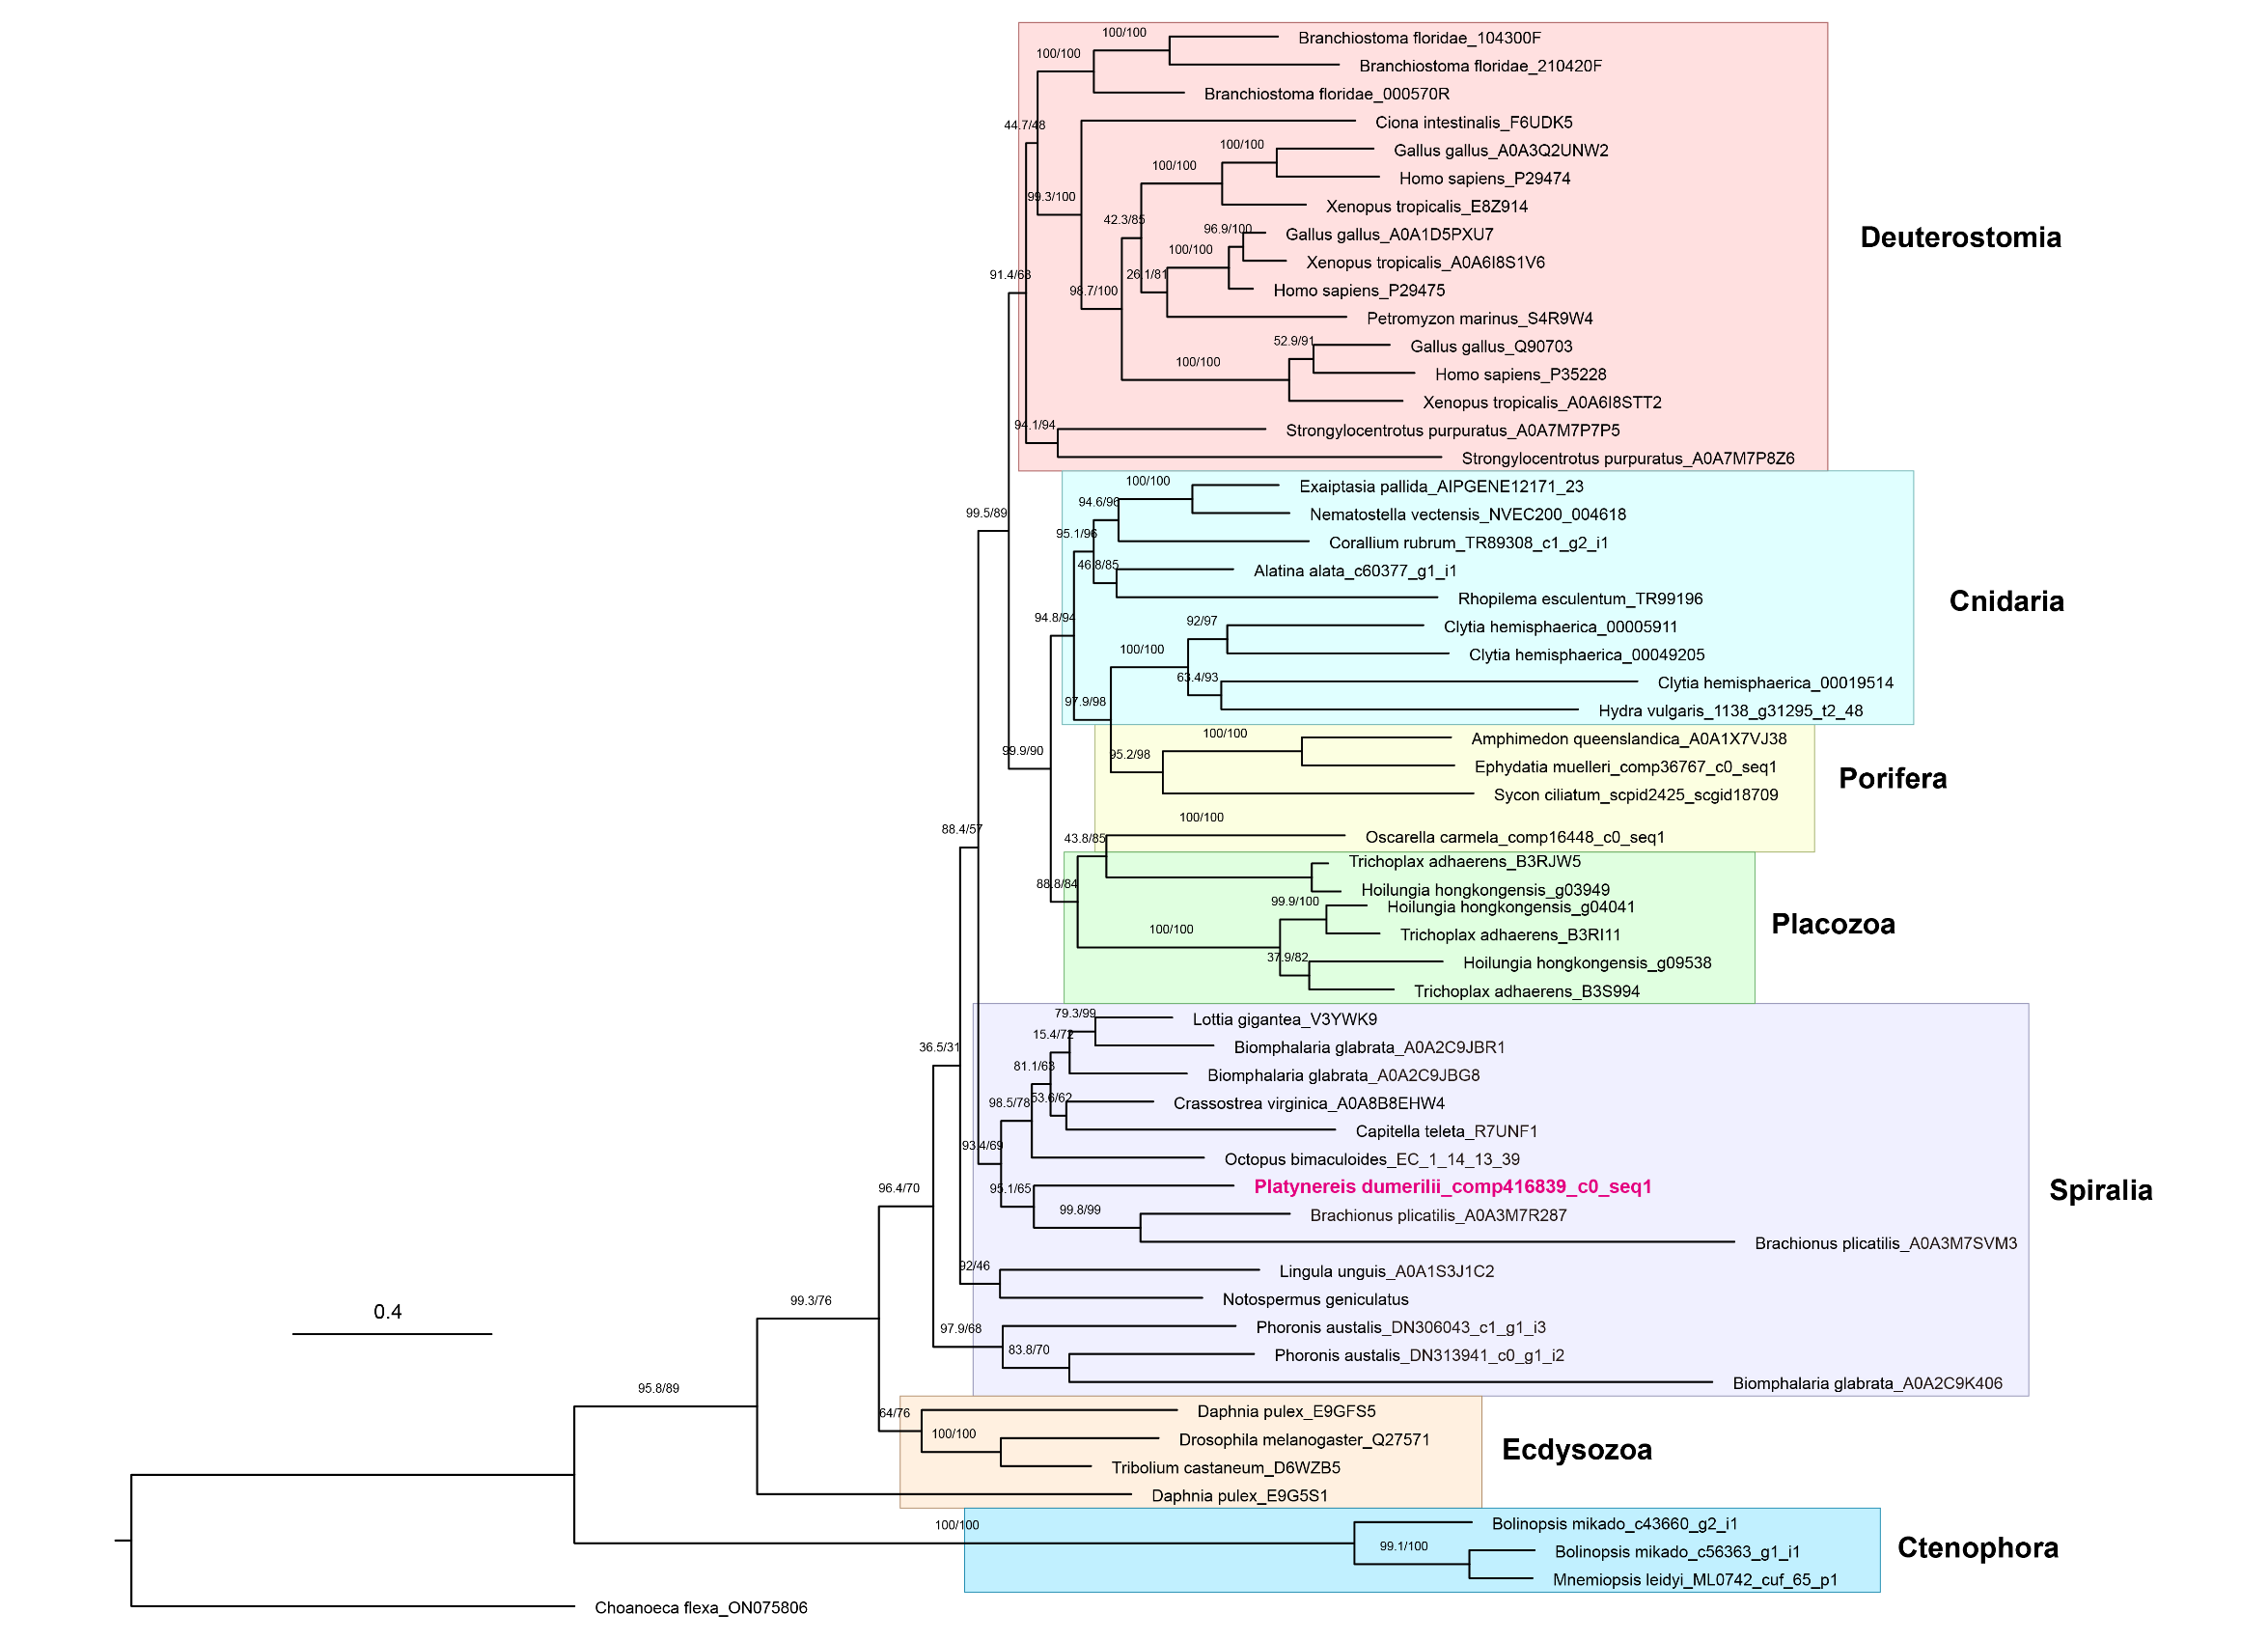
\includegraphics[width=27.78in]{figures/Fig1_sup1} \caption{**Figure 1 -- figure supplement 1**  Phylogenetic tree of NOS by maximum likelihood. Tree robustness was tested with 1000 replicates of ultrafast bootstrap with the aLRT-SH-like and aBayes methods.}\label{fig:unnamed-chunk-8}
\end{figure}

\begin{figure}
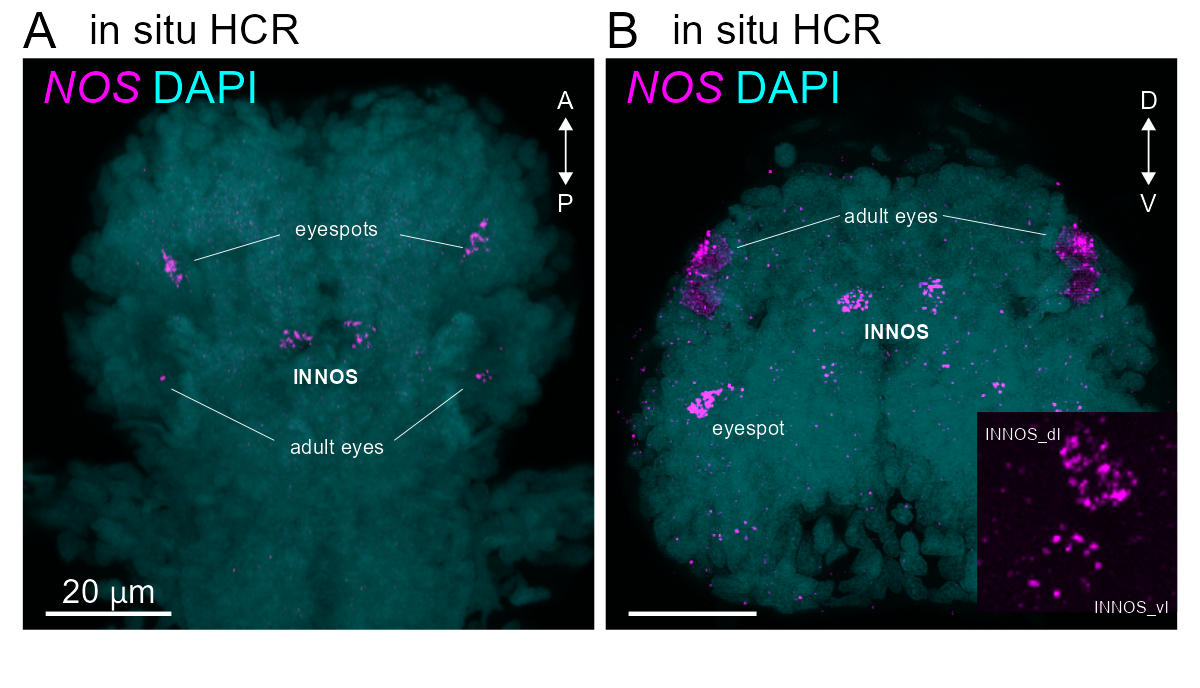
\includegraphics[width=16.67in]{figures/Fig1_sup2} \caption{**Figure 1 -- figure supplement 2** Expression analysis of the *NOS* gene (magenta) using in situ HCR using the larva at three-day-old in dorsal **(A)** and anterior view (B). (B) Insert: showing two NOS cells (INNOS_dl and INNOS_vl) on left side.}\label{fig:unnamed-chunk-9}
\end{figure}

\begin{figure}
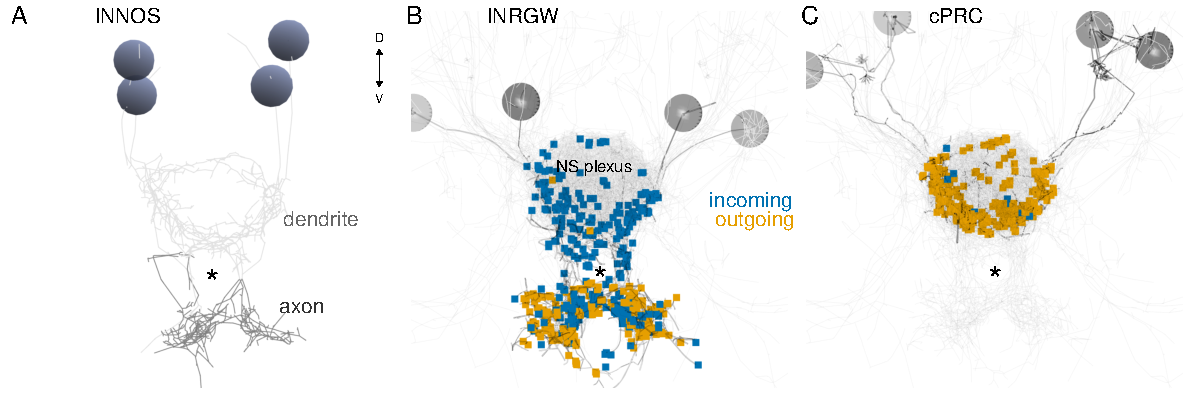
\includegraphics[width=43.06in]{figures/Fig1_sup3} \caption{**Figure 1 -- figure supplement 3** ssTEM reconstruction of the INNOS (A), INRGWa (B) and cPRC (C), anterior view. NS plexus; neurosecretory plexus}\label{fig:unnamed-chunk-10}
\end{figure}

\begin{figure}
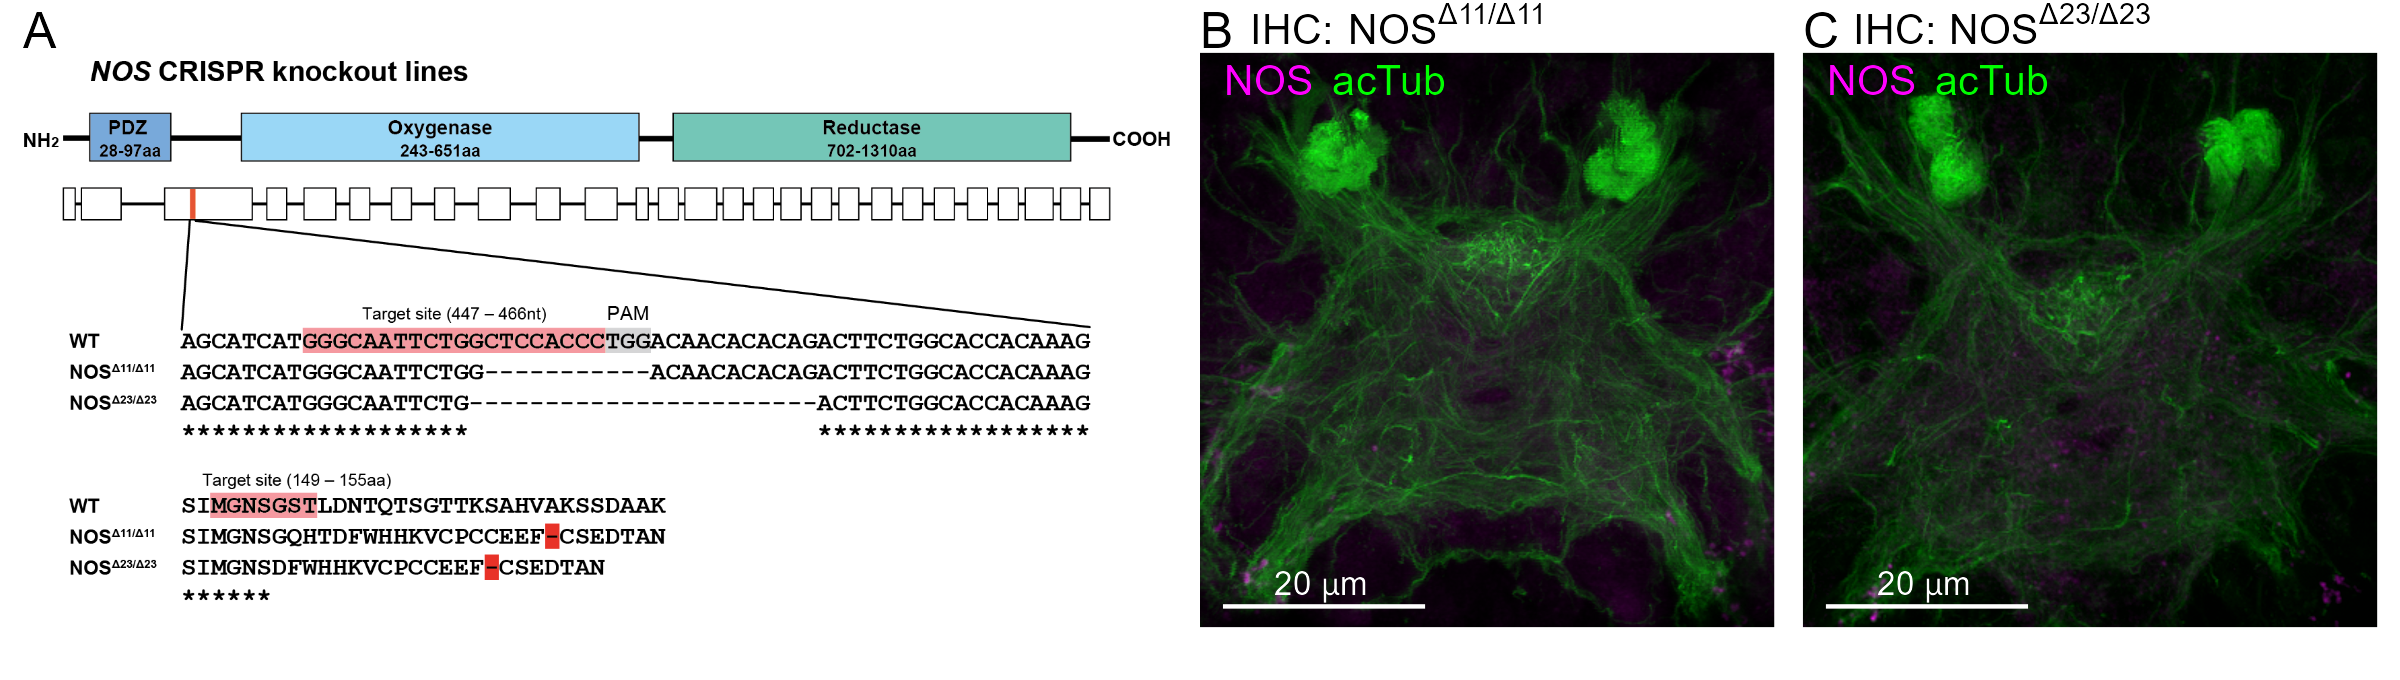
\includegraphics[width=44.44in]{figures/Fig3_sup1} \caption{**Figure 3 -- figure supplement 1** **(A)** Top: The domain and Exon/Intron structure of NOS. Bottom: Close-up region showing the genomic locus of NOS gene and the wild-type sequence (WT) targeted by CRISPR/Cas9. The generated mutants (NOSΔ11, NOSΔ23) are also shown. Pink indicates target sites. Gray shows PAM sequences, red shows stop codons. **(B)** Overlaid trajectories for WT (n=37) and NOS mutant (NOSΔ11/Δ11, n=18 and NOSΔ23/Δ23, n=8) at two-day-old larvae. 0 sec as the starting point. After 10 sec, UV (395 nm) stimulation from the side. **(C)** The temporal changes in the vertical position of the WT and mutant two-days-old larvae before and after UV stimulation are shown. The starting points of each larval trajectory are set to 0. After UV stimulation is indicated by purple squares. **(D, E)** The temporal changes in the distance traveled of the WT and mutant in two-day (D) and three-day-old (E) larvae before and after UV stimulation are shown. **(F)** The temporal changes in the distance traveled of larvae treated with NOS inhibitors, L-NAME in three-day larvae before and after UV stimulation are shown. **(G)** Vertical swimming in wild-type (WT) and mutant (NOSΔ11 and NOSΔ23) larvae at two-day-old stimulated with UV (395 nm) light from side, blue (488 nm) light from top and UV (395 nm) light from top. The data are shown in 30 s bins.}\label{fig:unnamed-chunk-11}
\end{figure}

\begin{figure}
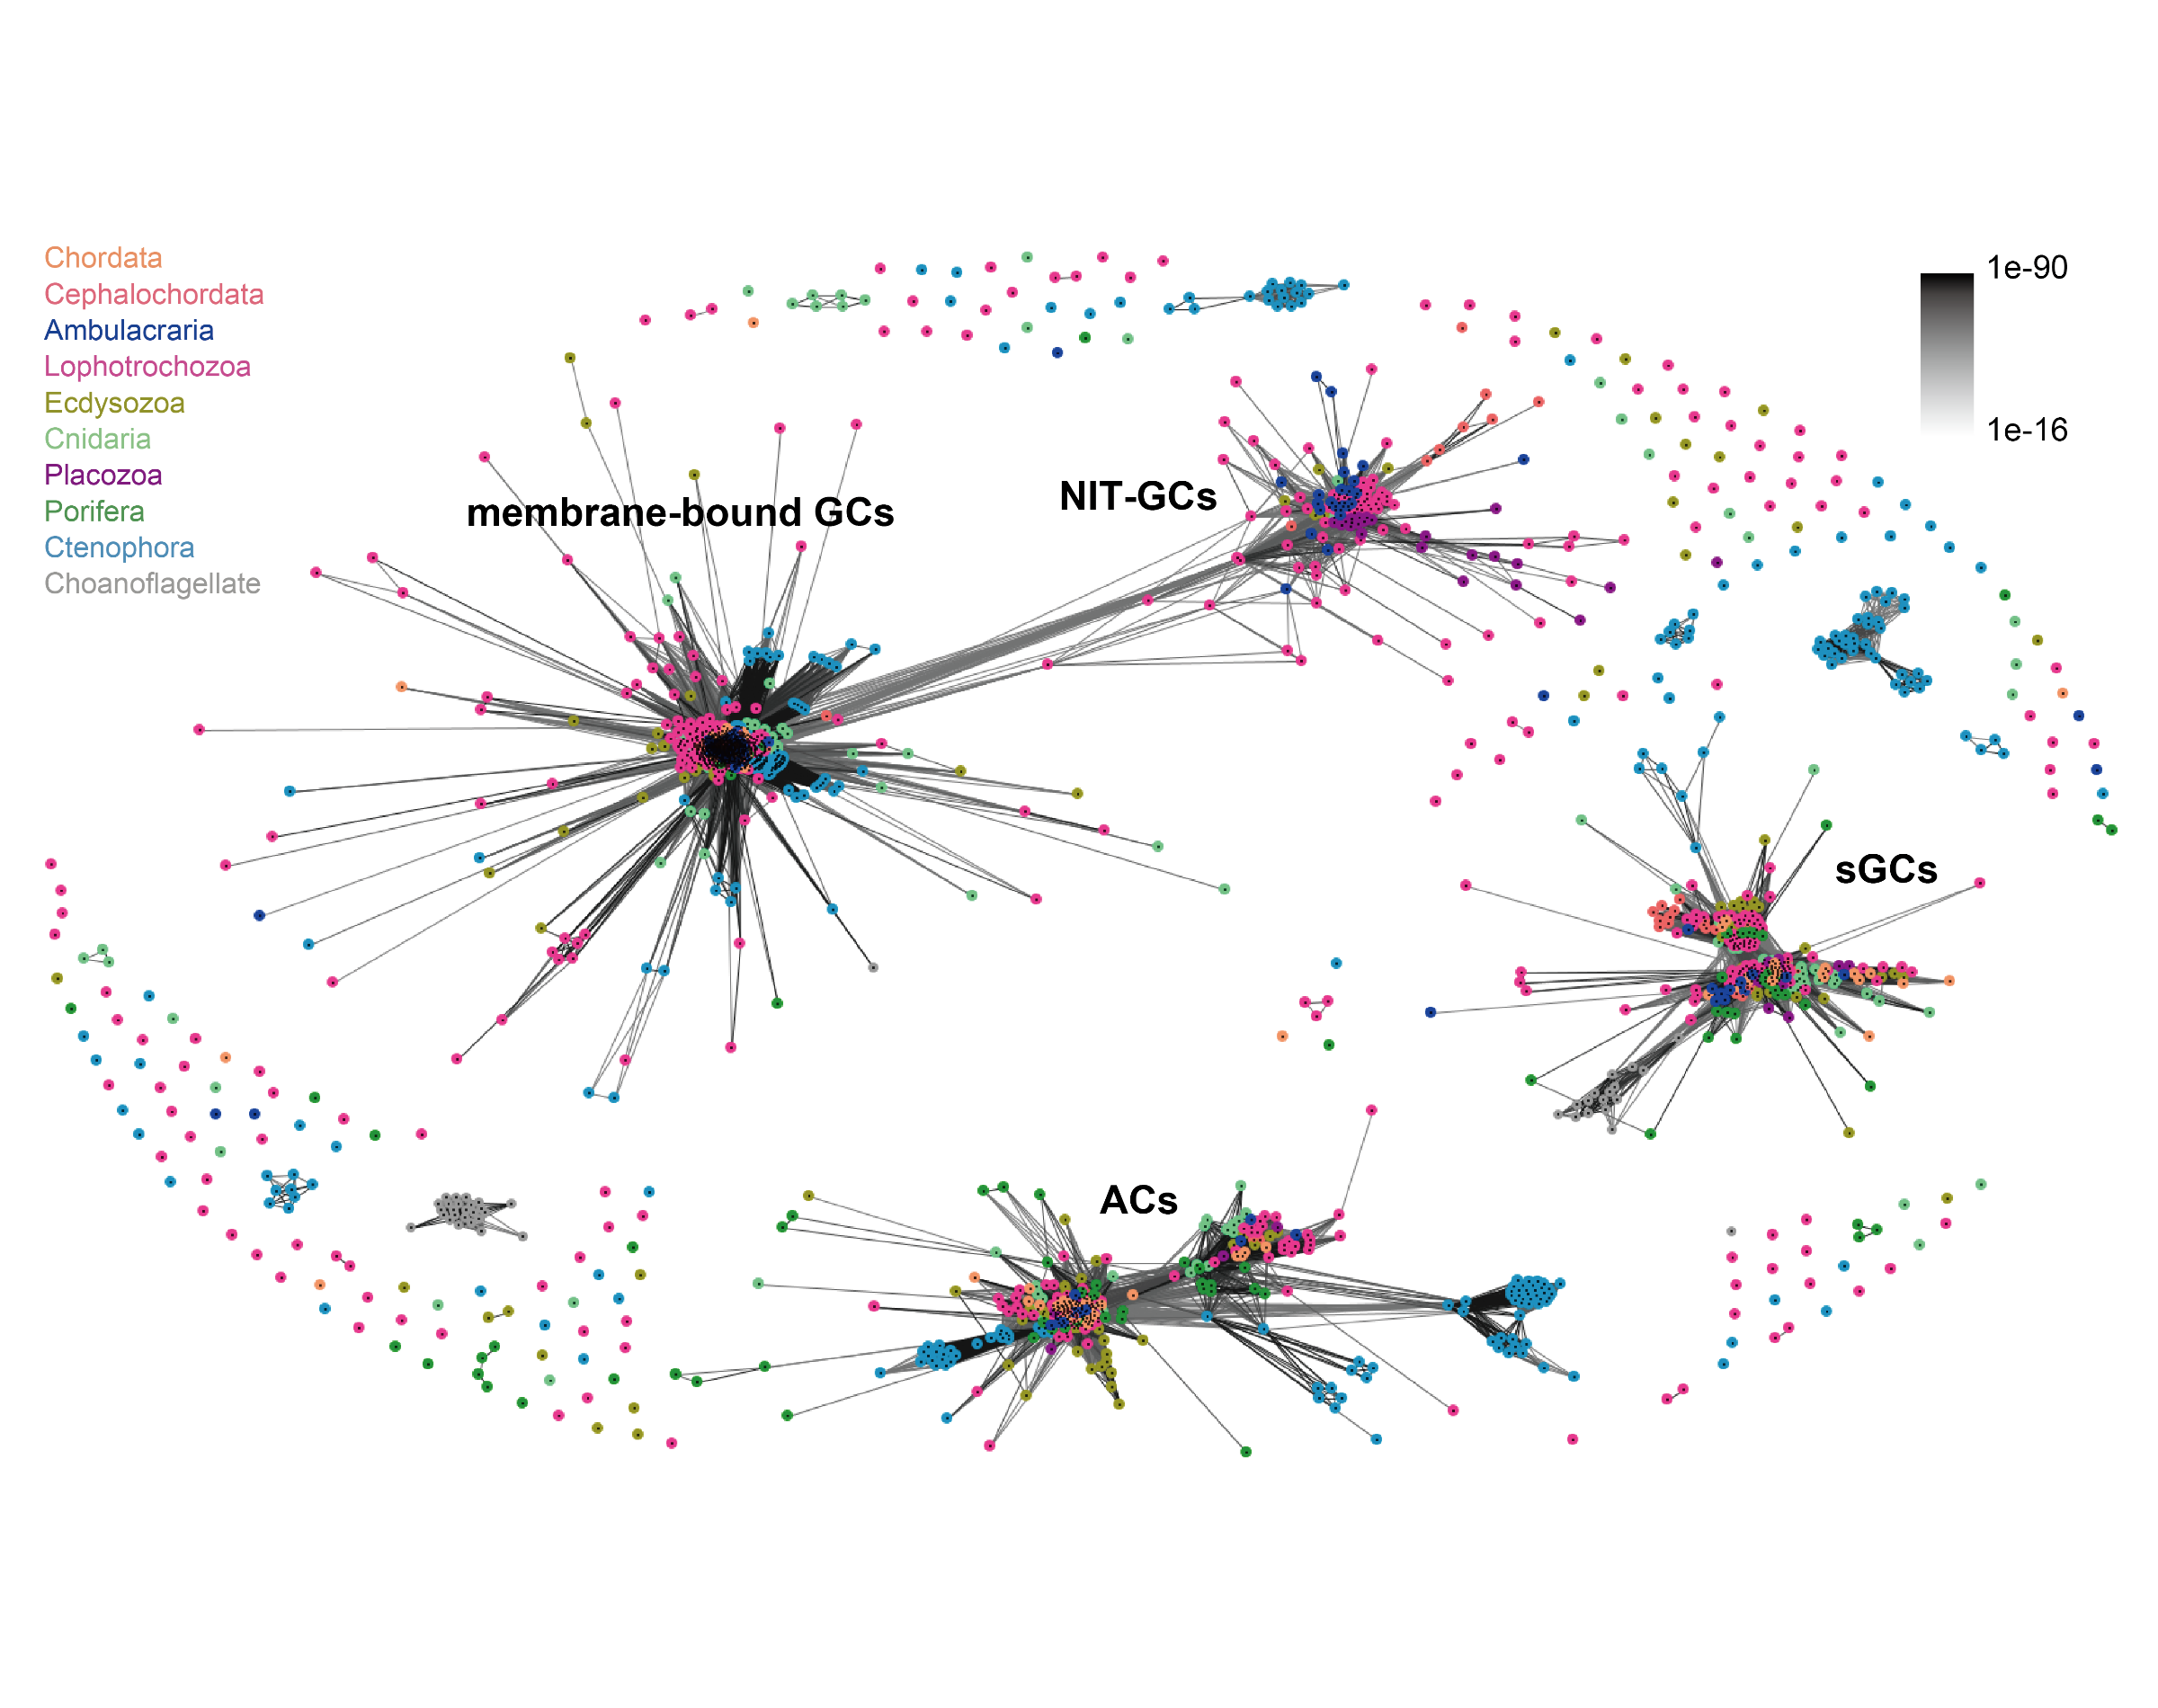
\includegraphics[width=33.33in]{figures/Fig4_sup1} \caption{**Figure 4 -- figure supplement 1** Cluster analysis of guanylate and adenylate cyclases. Connections are based on blast similarities < 1e-16 as shown on the upper right. Animal groups are colour coded as shown on the upper left. NIT-GCs, NIT domain containing guanylate cyclases; membrane-bound GCs, Membrane-bound guanylyl cyclases; sGCs, soluble guanylate cyclases; ACs, adenylate cyclases.}\label{fig:unnamed-chunk-12}
\end{figure}

\begin{figure}
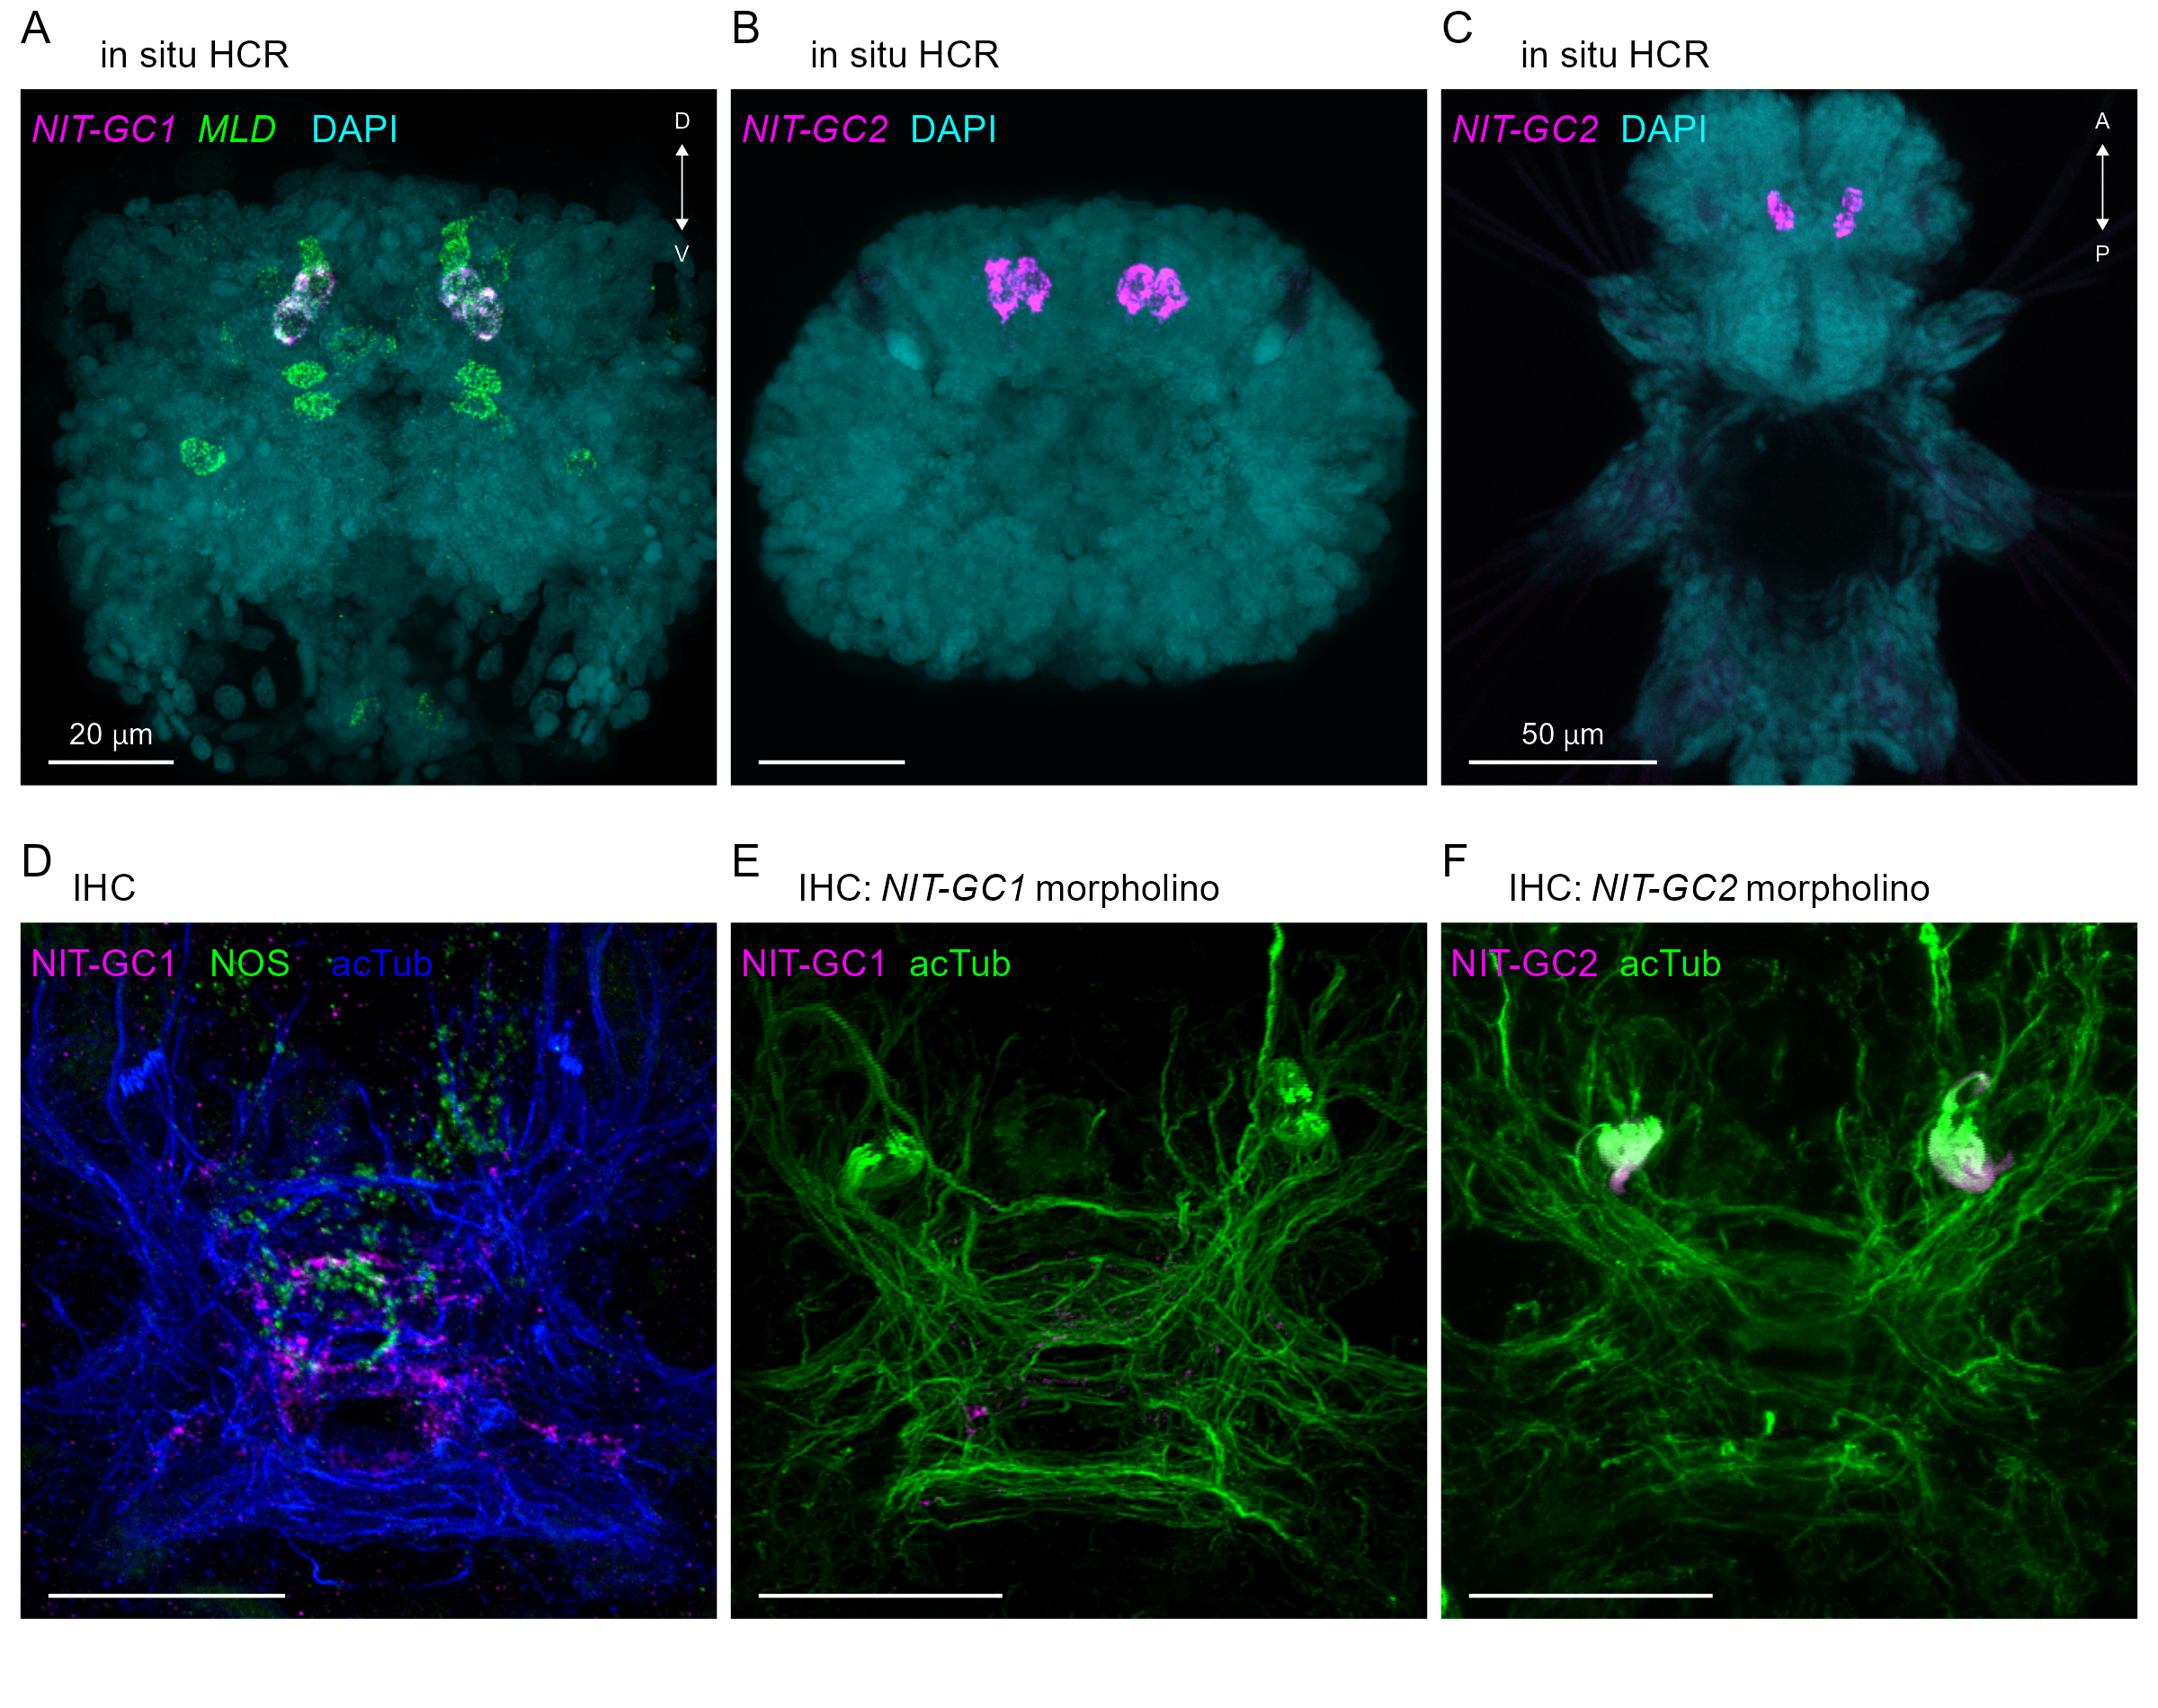
\includegraphics[width=20.83in]{figures/Fig4_sup2} \caption{**Figure 4 -- figure supplement 2** Phylogenetic tree of guanylate cyclase by maximum likelihood (ML). Guanylate cyclase-coupled receptor and soluble guanylate cyclases (sGC) as outgroups. Guanylate cyclases with NIT domains are found in most animal phyla except Porifera, Ctenophora, Urochordata and Chordata. Dot plot of Platynereis NIT-GC genes (columns) expressed in cPRC, INNOS and INRGWa (rows) using single cell RNA-Seq. The size of the dots is expressed in proportion to the percentage of cells expressing that gene relative to all cells. The colours represent the normal logarithm of the number of transcripts in the cells expressing the gene.}\label{fig:unnamed-chunk-13}
\end{figure}

\begin{figure}
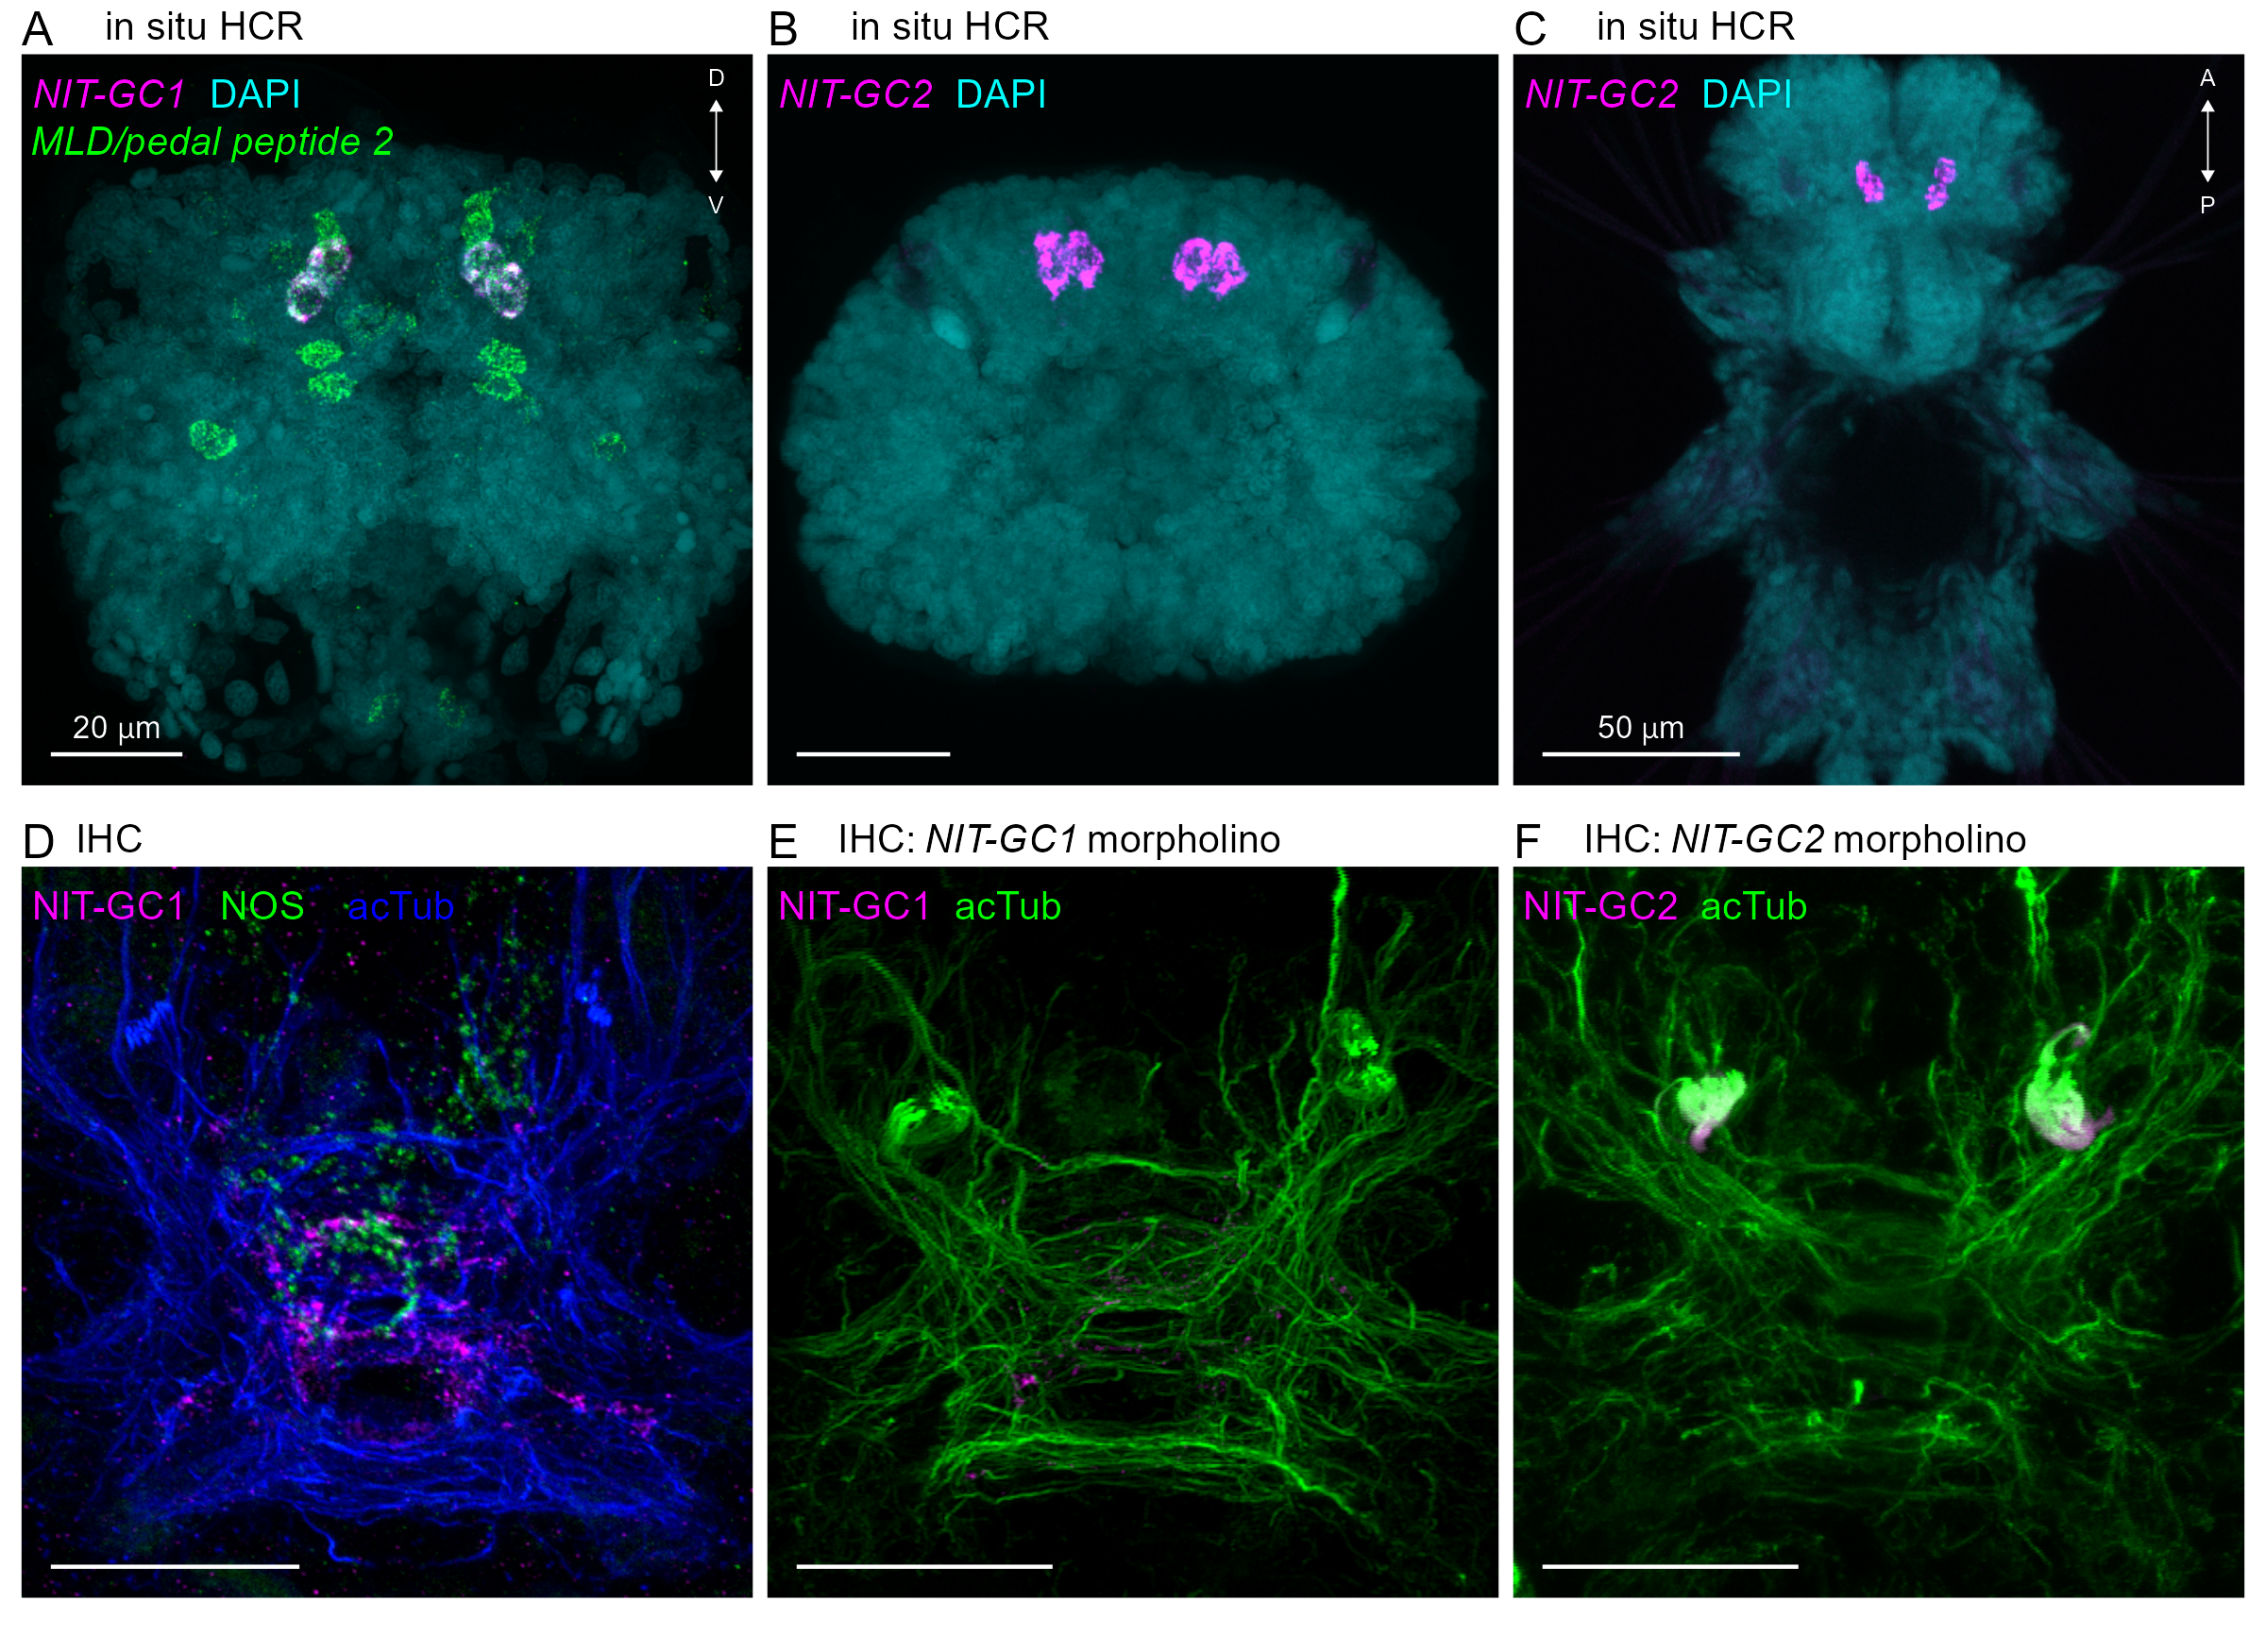
\includegraphics[width=33.33in]{figures/Fig4_sup3} \caption{**Figure 4 -- figure supplement 3** **(A)** Co-expression analysis image of the NIT-GC1 (magenta) and MLD-pedal2 amide proneuropeptide gene (MLD: green). Anterior view of the larva at two-day-old. **(B, C)** Expression analysis of the NIT-GC2 gene (magenta) using in situ HCR. Anterior (B) and posterior (C) views of the larva at three-day-old. **(D)** Co-localisation analysis using NIT-GC1 (magenta) and NOS (green) antibodies. Anterior view of the larva at two-day-old. **(E, F)** Localisation analysis using NIT-GC1 and NIT-GC2 antibodies for NIT-GC1 (E) and NIT-GC2 (F) morphant. Green shows co-staining with acetylated α-tubulin antibody (acTub). Anterior view of the larva at two-day-old.}\label{fig:unnamed-chunk-14}
\end{figure}

\begin{figure}
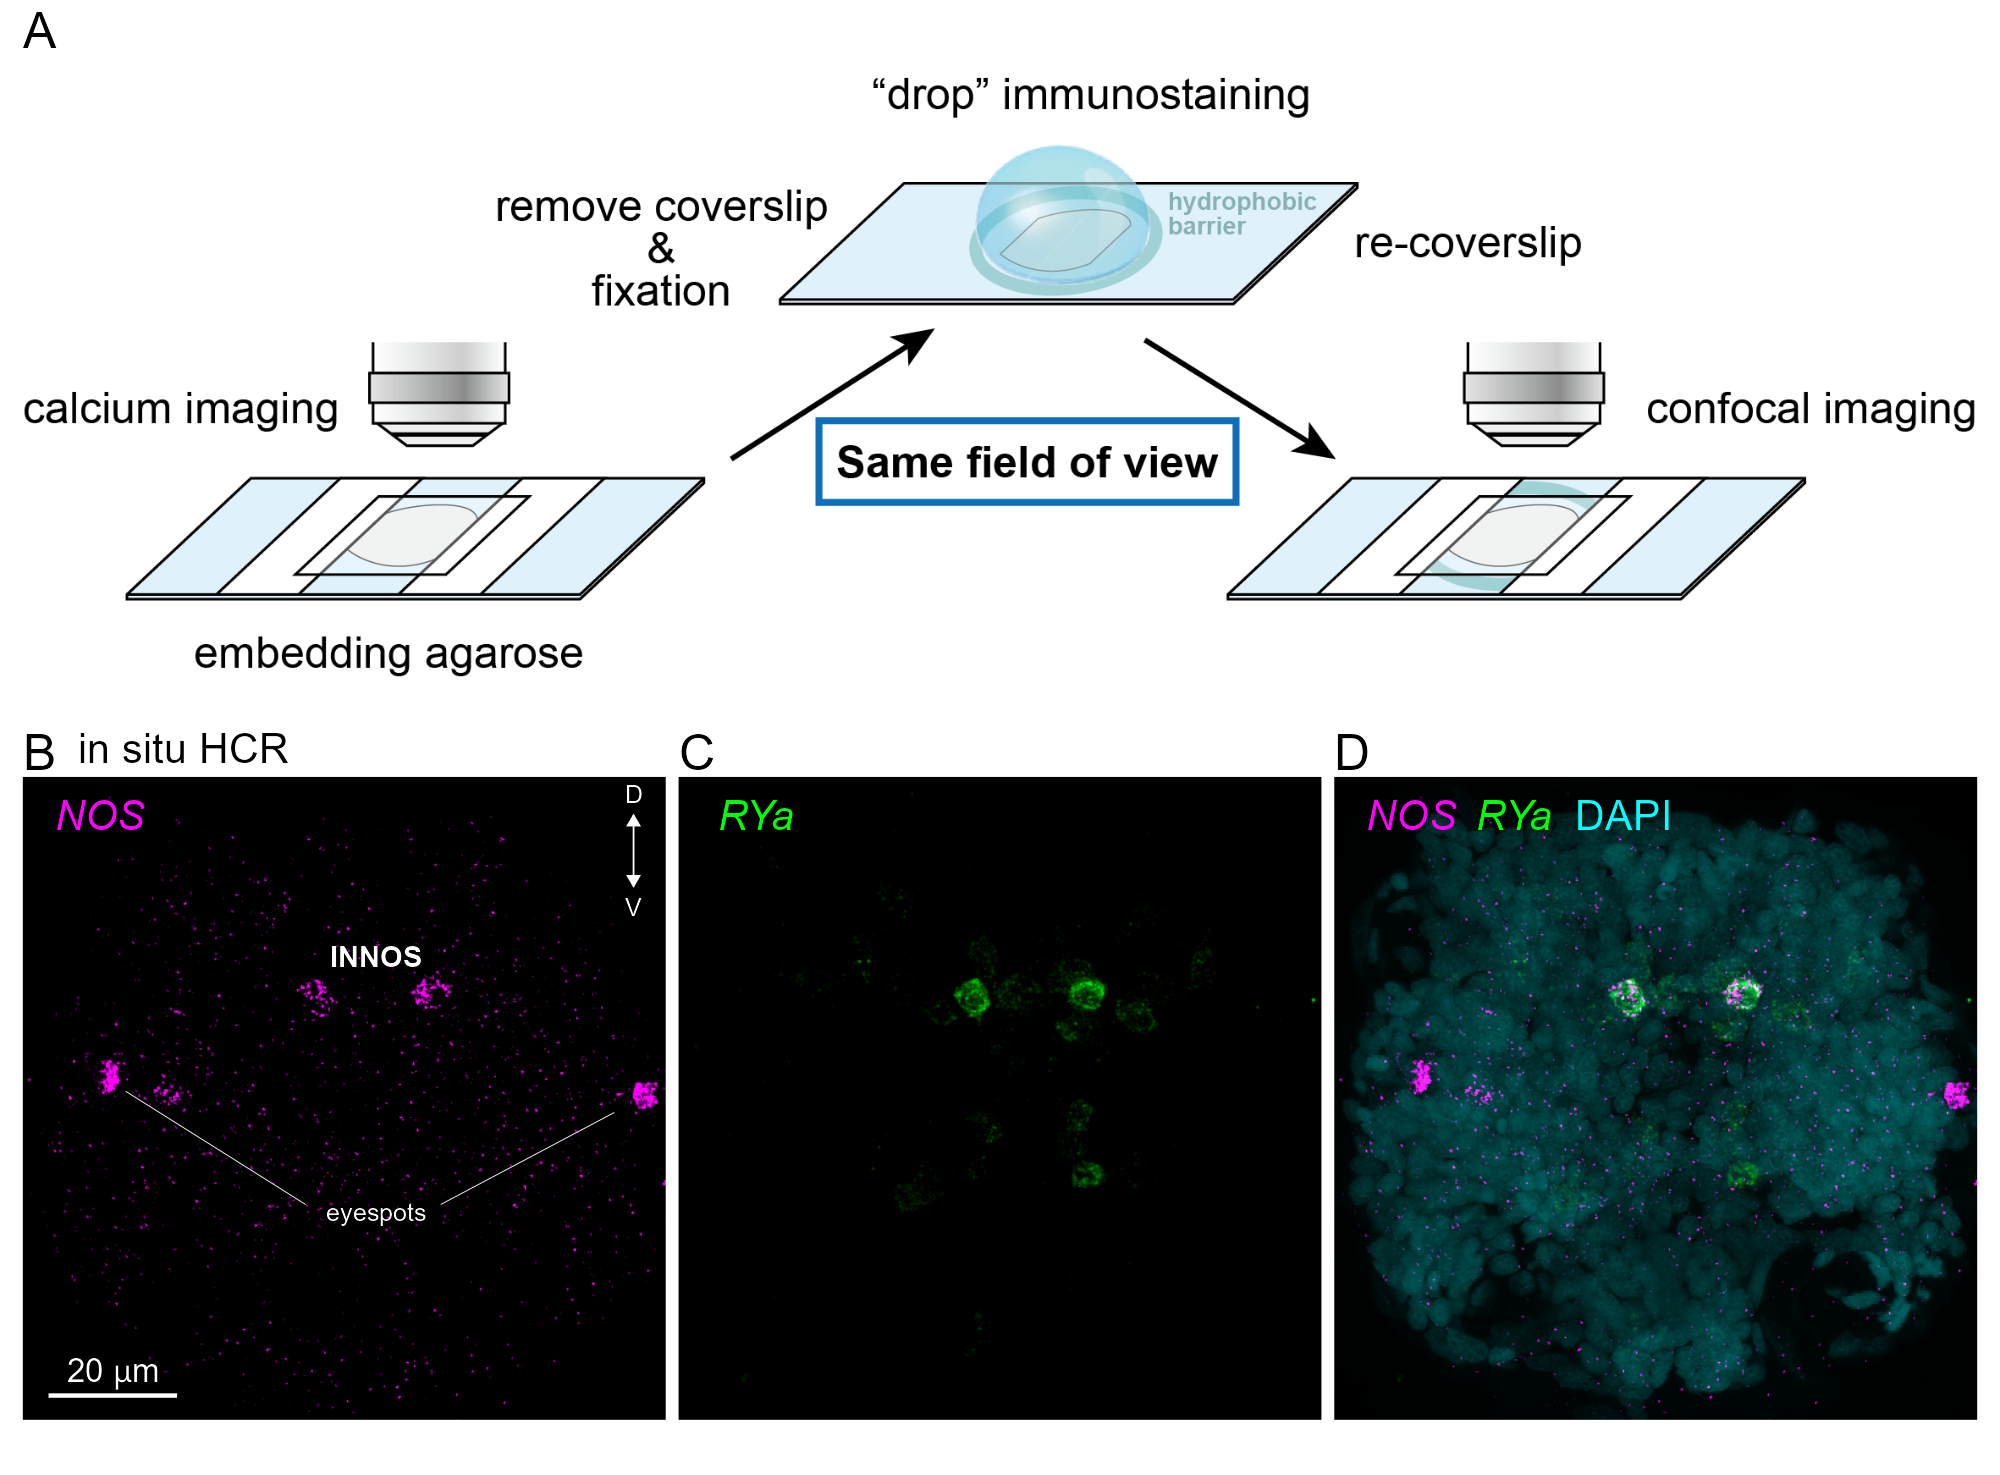
\includegraphics[width=27.78in]{figures/Fig5_sup1} \caption{**Figure 5 -- figure supplement 1** **(A)** Schematic diagram of the immunostaining procedure after calcium imaging.**(B-D)** Co-expression analysis image of the NOS (magenta) and RY amide proneuropeptide gene (RYa: green). Anterior view of the larva at two-day-old. }\label{fig:unnamed-chunk-15}
\end{figure}

\end{document}
